\documentclass[english, a4, 12pt]{scrartcl}
\usepackage{babel}
\usepackage[T1]{fontenc}
\usepackage[utf8]{inputenc}
\usepackage{lmodern}

\usepackage{subcaption}
\usepackage{wrapfig,graphicx}
\usepackage{placeins}
\usepackage{amsmath}
\usepackage{amsfonts}
\usepackage{dsfont}
\usepackage{enumerate}
\usepackage{graphicx}
\usepackage{mathrsfs}
\usepackage{braket}
\usepackage{color}
\usepackage[colorlinks=false, linkcolor=cyan]{hyperref}
\usepackage[ugly]{units}



\usepackage[singlelinecheck=off]{caption}
\setkomafont{captionlabel}{\bfseries}
\renewcommand*{\captionformat}{.~~}
\setcapindent{0pt}

\usepackage[backend=bibtex, style=numeric-comp, sorting=nty]{biblatex}
\bibliography{bib}

\definecolor{grey}{rgb}{0.9,0.9,0.9}

%\definecolor{forestgreen}{rgb}{0.0, 0.5, 0.0}
%\definecolor{orange}{rgb}{1,0.5,0}
%
\let\stdsection\section
\renewcommand\section{\newpage\stdsection}
\newcommand{\R}{\boldsymbol{R}}
\newcommand{\fata}{\boldsymbol{a}}
\newcommand{\K}{\boldsymbol{K}}
\newcommand{\bb}{\boldsymbol{b}}
\newcommand{\rr}{\textbf{r}} 
\newcommand{\p}{\boldsymbol{p}}
\newcommand{\kk}{\textbf{k}}
\newcommand{\diff}{\mathrm{d}}
\newcommand{\Z}{\mathbb{Z}}

%hilfmittelende

\begin{document}
\numberwithin{equation}{section}

	\begin{titlepage}
		\begin{minipage}[c][\textheight][c]{\textwidth}
			\begin{center}
				{ \Huge\textbf{Evolution of topological surface} }
				
				\vspace*{0.3cm}
				{ \Huge \textbf{states of thin HgTe-films with film} }
				
				\vspace*{0.3cm}
				{ \Huge \textbf{thickness} }
				
				\vspace*{1.5cm}
				{\Large \textbf{Bachelor thesis}}
				
				\vspace*{.7cm}
				{\Large Verfasst von Tamara Szecsey}
				
				\vspace*{.5cm}
				{\large \today}
				
				\vspace*{1cm}
				\hspace*{1cm} 
\includegraphics[height=30ex]{andere_bilder/urlogo}
				
				\vspace*{1cm}
				{\large Univeristät Regensburg}
				
				\vspace*{.3cm}
				{\large Fakultät Physik}	
							
				\vspace*{.3cm}
				{\large Im Bereich theoretischer Festkörperphysik}
				
				\vspace*{.7cm}
				{\large Unter der Betreuung von}	
				
				\vspace*{.3cm}
				{\large Prof. Dr. Ferdinand Evers}
				
				\vspace*{.3cm}
				{\large und}	
				
				\vspace*{.3cm}
				{\large Maria Camarasa-Gomez}									
			\end{center}
		\end{minipage}
	\end{titlepage}

\thispagestyle{empty}
Ich habe die Arbeit selbständig verfasst, keine anderen als die angegebenen Quellen und Hilfsmittel benutzt und bisher keiner anderen Prüfungsbehörde vorgelegt. Außerdem bestätige ich hiermit, dass die vorgelegten Druckexemplare und die vorgelegte elektronische Version der Arbeit identisch sind, dass ich über wissenschaftlich korrektes Arbeiten und Zitieren aufgeklärt wurde und dass ich von den in § 24 Abs. 5 vorgesehenen Rechtsfolgen Kenntnis habe. 
\newpage
\thispagestyle{empty}
\tableofcontents	
\clearpage	
\setcounter{page}{1}
\section{Introduction}
	During the last ten years, topological insulators were the most examined topic in condensed matter physics. These materials are insulating in their interior, also known as the bulk, but possess conducting surface states. This quality makes it very exotic and attractive for potential applications. Therefore big effort was made in order to find materials of this kind. One of these is HgTe for which we studied the evolution of topological surface states in this thesis \cite{top_surf_states}. 
	
	More explicit, we concentrate us on the topological surface states in the surface growing direction (001). We approach this problem by performing ab-initio calculations, in detail, we used density functional theory (DFT) through the commercial package FHI-aims. 
	
	By combining the supercell approach and the projected bulk band structure we observe how sensitive the energy band structure, as well as the surface states react on different thicknesses and terminations of the slabs. 
	Additionally we thus will see the evolution of the surface states in this material regarding the (001) plane. 
	
	This thesis is divided into five parts: In part one we give an introduction of the main topic. In part two we give an explanation of the theoretical background including the concept of topological insulators, the basic principles for numeric modeling of surfaces by applying density functional theory and the origins of spin-orbit interaction in solid state matter.
	In part three of this thesis we present the results of our calculations for the slab band structure of HgTe with various thicknesses and in cases of ideal and passivated surfaces.
	In part four we interpret those results. And finally in part five we close this thesis by conclusions. 
		
%	This thesis treats a new field in condensed matter physics which was first identified by J. M. Kosterlitz and D. J. Thouless in 1972 which received the Nobel prize \cite{nobel_prize} in 2016 for topological phases of matter, in other words, the transfer of the mathematical concept of topology into condensed matter physics. 
%	
%	Then this concept was further investigated until the two-dimensional topological insulators (TIs) where introduced by Kane and Mele. These specific insulators form a new quantum state of matter and enjoys great interest in condensed matter physics because of it's exotic properties and potential applications. 
%	
%	One topological insulator, that could be observed due to it's big band gaps, was HgTe as quantum well. This material has an inverted band structure due to the spin momentum locking in tellurium (Te) and to the spin-orbit coupling correction in the bands of mercury (Hg), which distinguishes it from normal insulators. 
%	
%	But the concept of TIs can also be transfered to the three-dimensional space, which was examined in this thesis for very thin layers of HgTe. The observations were made by a computational method: the DFT-PBE method, calculated by the program FHI-aims, version 081912 for calculations without spin-orbit coupling, meaning k-grid and lattice constant study, and version 160328\_3 for calculations with spin-orbit coupling.
%	
%	The thesis is divided in five parts, the introduction, the theory, which includes closer explanations of the topological insulators, fundamental knowledge about crystals and solid state matter, introduction into the surface modeling in computational physics, the density functional theory and the spin-orbit coupling. The third part includes the results of the calculations, including the simulated growth of the HgTe crystal in z-direction. The band structures and the density functional gives informations about the band inversion property and occupation number in the HgTe slab. In the end there is a section interpreting the results and the conclusion which closes this thesis. 
	
\FloatBarrier
\section{Theory}
	\subsection{Topological insulators}
	% What they are, types and characteristics
%	\begin{figure}[tbp]
%		\begin{minipage}[c]{.48\linewidth}
%			\centering
%			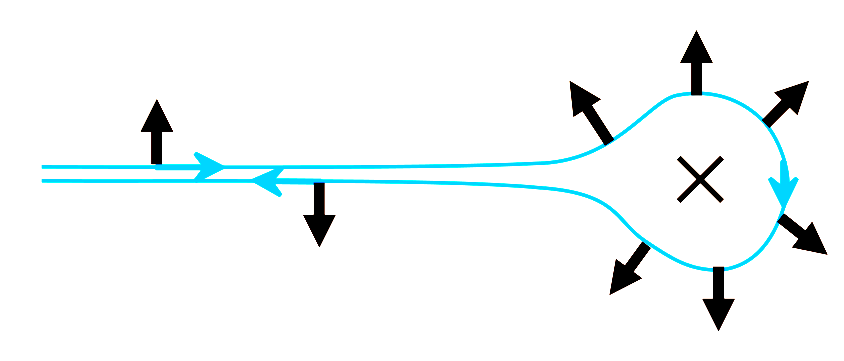
\includegraphics[width=\linewidth]{electron_spin_reflection_1.png}	
%		\end{minipage}
%		\hfill
%		\begin{minipage}[c]{.48\linewidth}
%			\centering
%			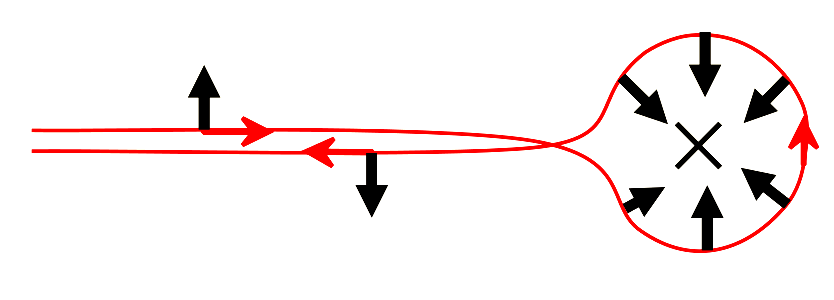
\includegraphics[width=\linewidth]{electron_spin_reflection_2.png}	
%		\end{minipage}
%		\caption{Two different ways of an electron's spin is been reflected off an impurity, which has no magnetic momentum. Both are turning the spin from $\pi$ to $-\pi$ which is a difference of $2\pi$, thus the spins destruct each other and ensure perfect transmission. The time-reversal symmetry is hence guaranteed. (Picture from \cite{topological_insulators}) } \label{electron_spin_reflection}
%	\end{figure}
%	They can be classified by topological order into trivial and non-trivial insulators. The latter ones contain conducting states at the surface.  

%	Insulators in general are in lack of freely flowing electric charges so that no current flows under influence of an electric field. But under sufficiently large voltage, an insulator still becomes conductive by tearing the electrons away from the atoms. Experimentally this means, that they have a higher resistivity than semi-conductors and conductors. 
%
%
%	The concept of topological insulators (TIs) was first predicted in two dimensional space, more specific, the predictions are related to quantum spin Hall (QSH) edge states in graphene band structures discovered by Kane and Mele \cite{Kane_Mele1} by applying spin-orbit coupling (SOC) (see subsection \ref{chapter_soc}). The SOC including gave rise to a gap opening where graphene normally has no gap in its Dirac band structure. But this gapping is different than the ones of normal semi-conductors. Namely the band ordering is inverted and this inversion is different for an opposite spin. This comes from the spin-momentum locking, which means, spin and momentum remain perpendicular to each other. Additionally prevents backscattering for the QSH edge states. If a flowing electron is back scattered by a non-magnetic impurity, it will act destructively on the incoming one. This is illustrated in figure \ref{electron_spin_reflection}. The physical designation the two QSH edge states which are moving in opposite direction is a Kramers douple, and the phenomenon of prohibited backscattering is due to the protection of the time-reversal symmetry. 
%	That symmetry can be broken by e.g. an magnetic impurity which opens a gap without QSH edge states. 
%	
%	Since this means that material with that property differs from other insulators by their topological order, Kane and Mele \cite{Kane_Mele2} introduced the topological invariant $\Z_2$, which can be broken down to two simple integers 0 and 1, trivial and non-trivial TI. This gave rise to the name 'topological insulator', where either there are QSH edge states protected by time-reversal symmetry or the time-reversal symmetry is broken and there is a band gap with no QSH states.
	Originally, materials were named conductors if, by applying an electric field or an insulator, small electric currents start to flow as a reaction to the external field. 
	
	But 2005 Kane and Mele \cite{Kane_Mele1} discovered that apart from the insulators, the conductors and the semiconductors, there is an other class of material: the so-called topological insulator, which acts like an insulator in the inner part (bulk) but is conductive at the surface. 
	Additionally the surface states of these topological insulators are special in comparison with normal surfaces since they are symmetry protected by time-reversal symmetry and because of their band structure. 
	
	From a practical point of view topological insulators arise by combination of spin-orbit interactions, which itself provide spin-momentum locking and band inversion, and closed energy bands. Because of the spin-momentum locking, backscattering is not possible for surface states as long as time-reversal symmetry is preserved. The reason is, that the spin can not change while the momentum doesn't. 
	The band inversion is the origin for the characteristic Dirac cones of the surface states which lie between the band gap.
	A sketch of one Dirac cone on the surface is illustrated in figure \ref{band_structure_top_insulator}.
	Note that the surface states cannot be removed by modification, i.e. by passivation or disorder, as long as time-reversal symmetry is preserved. 
	
	In 2D a topological insulator possesses 1D edge channels which are counter propagating and spin polarized \cite{Kane_Mele2}. They are known as quantum spin Hall edge states and were first predicted in graphene \cite{Kane_Mele2} but later were found in HgTe quantum wells \cite{Bernevig}. 
	
	Quantum wells have non-trivial topological surface states under a certain critical thickness but become trivial insulators as soon as they pass this critical thickness. 
	\begin{figure}[b!]
		\centering
		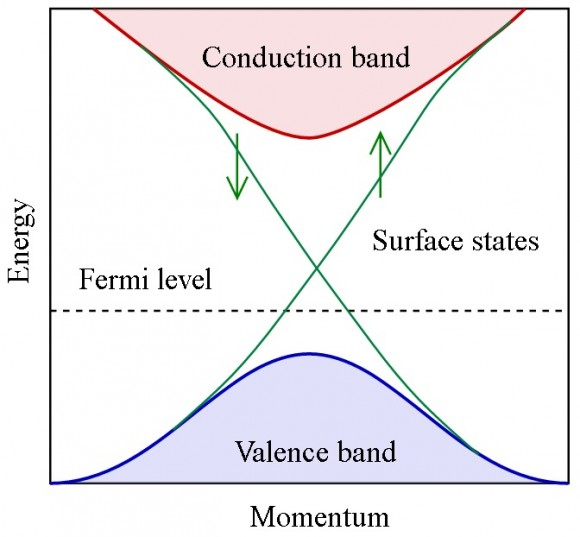
\includegraphics[width=0.4\linewidth]{andere_bilder/band_structure_top_insulator.jpg}
		\caption{%Band structure near the Fermi level for a topological insulator. Due to spin-momentum locking, the surface states are protected. The electrons can flow so well, that the surface is conductive
			Sketch of band structure of a topological insulator near the Fermi level (dashed lines). In blue: valence band, in red: conduction band, in green: the surface states with nearly linear dispersion close to the Fermi level. Each branch of the Dirac cone have opposite spin polarization in respect to the other branch. 
			(Picture from \cite{wiki_top_ins})} \label{band_structure_top_insulator}
	\end{figure}
	
	The prediction was closely followed by the generalization of the concept of topological insulators on to 3D. 
	In this dimension there are two different kinds of topological insulators which are defined by the band structure characteristics: There are strong topological insulators which have an odd number of Dirac cones in the bulk band structure and there are weak ones with an even number of those Dirac cones. 
	
	HgTe, which is the material we consider in this thesis, is also a 3D topological insulator under certain circumstances. In general it is a semi metal, but under applied strain its $\Gamma_6$ and $\Gamma_8$ bands close up at the Fermi level \cite{textbook_ti}. This was confirmed by experimental ARPRES and tranport measurements.
	
	An interesting question is what happens to the band structure and the topological properties by applying strains in one direction. This question will be partly answered in the following sections.
%	But for graphene, the band gap predicted is too small and shows up just at very low temperature, which makes it impossible to observe with todays technical equipment.  
%	In contrast these properties were found in HgTe quantum wells. 
%	A quantum well is a potential with only discrete energy values. Experimentally this can be obtained by stealing one degree of freedom from original free movers in three dimensional space, so that they just can move in a plane.
%	For HgTe this is obtained by sandwiching it between a material that has larger band gaps, which in addition always needs to be thicker than the HgTe in the middle. 
%
%	Above the critical thickness $6.5 \,\unit{nm}$, the HgTe quantum well develops topologically non-trivial states, i.e. the QSH states, with reversed conduction and valence band. Below that thickness the bands are normally ordered and it has topologically trivial states, that is to say a normal band gap. 
%	
%	The concept of topologically protected states can be transfered to three dimensional systems with four different topological $\Z_2$ invariants (Moore and Balents \cite{Moore}). Fu, Kane and Mele \cite{Fu_Kane_Mele} categorized the non-trivial topological states into weak and strong ones, according to their robustness against disorder. HgTe is a strong one and thus develops surface states with an odd number of Dirac cones while the bulk, the inner part of the metal, is insulating. 
%	
%	Those surface states are very similar to the QSH edge states, where the latter are one dimensional states in two dimensional space and the earlier are two dimensional states in three dimensional space. The Dirac cones which live in the $\kk$-space, are those surface states where the spin rotates with $\kk$ around the Fermi surface as long as time-reversal symmetry is conserved. The manifestation of the a Dirac cone in the band structure looks as shown in figure \ref{band_structure_top_insulator}.  
%	The simplest case is a single Dirac cone, which is the case for HgTe. 

%	The topological insulators are solid materials made out of heavy elements which are insulating at the inner part but conducting at the surface. Additionally they have surface states which are protected by particle number conservation and time-reversal symmetry. 
%	
%	The characteristic band structure of a topological insulator is illustrated in figure \ref{band_structure_top_insulator}. The surface states colored in green arise because of the band inversion of the valence band and the conduction band which is induced by the spin momentum locking. And this again arises of to the strong spin-orbit coupling (SOC) which are induced by the relativistic effects of heavy elements.
%	
%%	This means the spin and the momentum are always normal and thus the electrons can just go those two ways. 
%	This surface state structure is called a Dirac cone and is additionally protected by time-reversal symmetry.
%	This means, if an electron is reflected by an non magnetic impurity, the spin gets reflected by a rotation of $2 \pi$, so that it can act destructively on the incoming electron, see figure \ref{electron_spin_reflection} for illustration.
%	In contrast, true magnetic impurities can destroy those surface states because the rotation would be in a way, that the reflected electrons are no longer destructing the incoming ones.
%	 
%	Because there are two ways of reflecting destructively, see blue and red lines in the figure, there are two ways of conserving the time-reversal symmetry. 
%	\\\\	
%	%		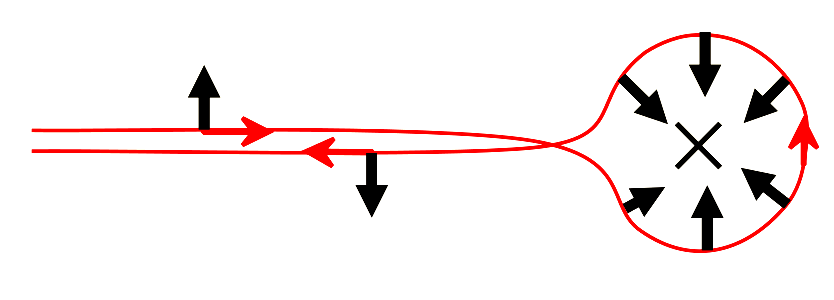
\includegraphics[width=\paperwidth]{electron_spin_reflection_2.png}
%	The underlying ways of defining the topological insulators are the noninteracting topological band theory \cite{Kane_Mele1} \cite{Moore} \cite{Roy}, which relies on the quantum spin Hall effect and the topological field theory \cite{Hughes_Zhang} \cite{Qi}, where the effective Maxwell action which describes the insulator's electron response, is rewritten in a way, that it no longer depends on the geometry of the insulator, but on it's topology.
%%	\begin{equation} \label{Maxwell_action}
%%		S_{\text{Maxwell}} = \frac{1}{16 \pi} \int \diff^3 x \,\diff t 
%%		\left(\epsilon \vec{E}^2 - \frac{1}{\mu} \vec{B}^2\right)
%%	\end{equation}
%%	with $\epsilon$ being the electric permittivity and $\mu$ the magnetic permeability, can be rewritten in dependence on a parameter $\theta$ \begin{equation}\label{topological_action}
%%		 S_\theta = \frac{\theta \alpha}{4 \pi^2} \int \diff^3 x\, \diff t \vec{E} \cdot \vec{B}
%%	\end{equation} 
%%	with $\alpha= e^2/\hbar c$, which only can accept two different values for preserving time-reversal symmetry, $\theta = 0$ or $\theta =\pi$. This implicates, that this action no longer depends on geometry, but on the topology. 
%	
%	Both ways of defining the types of topological insulators are leading to the so called $Z_2$ classification similar to the genus in topology. This means, every insulator of this kind can be categorized by an explicit topological invariant that can only give binary values of 0 and 1. 

%%% Local Variables:
%%% mode: latex
%%% TeX-master: "main_BA2.0"
%%% End: \label{topological_insulator}
	
	\subsection{Description of a crystal structure}
		\FloatBarrier
	\begin{figure}[tbp]
		\centering
		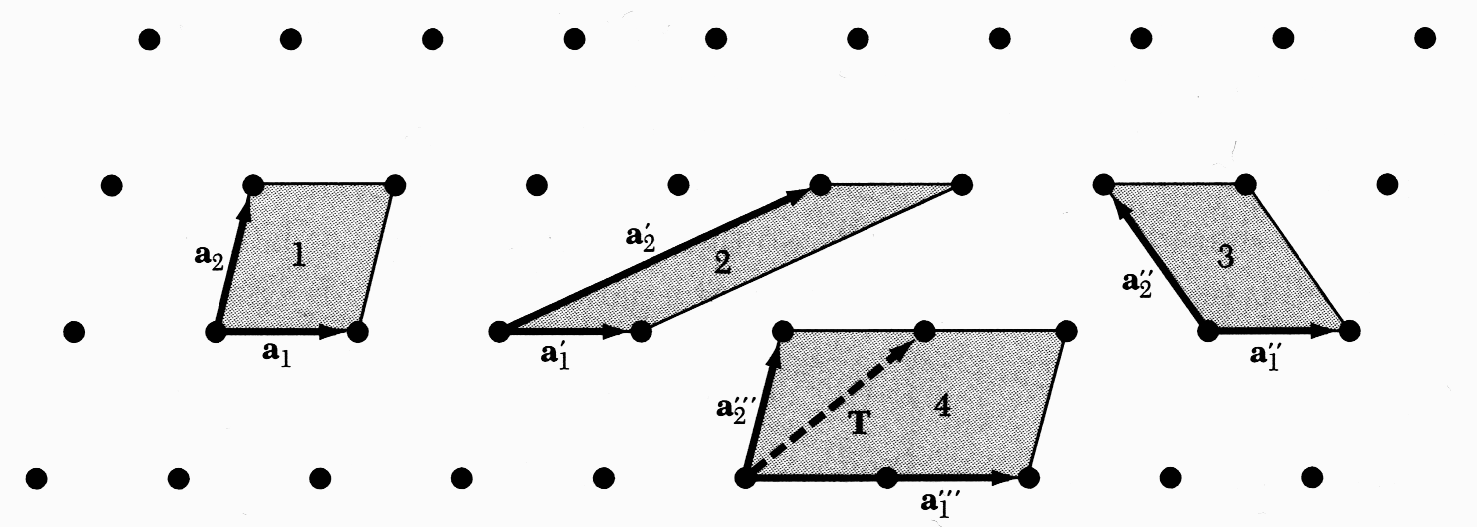
\includegraphics[width=.9\linewidth]{andere_bilder/basis_2dim.png}
		\caption{Some two dimensional unit cells with different basis vectors. The cells 1,2 and 3 are primitive unit cells, but 4 
%		isn't because it is twice as big as 1.
		is not because its volume is twice as big as, for example, the parallelogram number 1. For a primitive cell it must be verified that the volume is as small as possible in order to reproduce the lattice when repeated in space in all directions considered. 
		(Picture from\cite{Kittel})}\label{basis_2dim}
	\end{figure}
	%crystals, bulk, surfaces, band structures. What they are? Talk about the Brillouin zones and the real and reciprocal space. How are they related to each other?
%	-unendliches Gitter-> bulk
%	-Wigner-Seitz->primitive einheitszelle
%	-Bravaisgitter
%	-sc,bcc,fcc,diamand struktur
%	-millersche indizes
%	-zinkblendestruktur
%	-reziproker raum
%	-Brillouin zonen
%	-band structure
%	-surfaces

%	In solid state physics, the characteristics of the inner part of a finite crystals are approximated by infinite lattices. This part of a solid, where the surfaces are not regarded, is called the bulk. 
	A crystal structure describes the arrangement of atoms in a crystalline material. The atoms out of which a crystal is made, maintain a symmetric pattern repeating itself into the three spatial dimensions. 
	
%	\subsubsection{General description of the crystal structure}
	For this reason, to describe the crystal structure, one needs a basis, which can start at any atom $i$ in the lattice, in order to form a unit cell. For a three dimensional crystal, we need a three dimensional lattice and to describe the crystal lattice we introduce three primitive translation vectors $\fata_1,\fata_2$ and $\fata_3$. These vectors indicate the directions where to the atom $i$ of the crystal, which holds the coordinates $x_i, y_i $ and $z_i$, must be replicated in order to compose the whole crystalline structure. The crystal translation vector $\boldsymbol{R}_i$ is then defined as 
%	three basis vectors in need $\fata_1,\fata_2, \fata_3$ so that the structure is given by:
	\begin{equation} \label{vector}
		\boldsymbol{R}_i = x_i \fata_1 + y_i \fata_2 + z_i \fata_3
	\end{equation}
	There are different ways to choose the basis set for the unit cells, some possible choices for a two dimensional lattice are illustrated in figure \ref{basis_2dim}. In this figure one can also see some unit cells, shown in grey areas, that, with the exception of 4, are primitive unit cells.
%	Some examples of how to choose a possible basis set for a two dimensional lattice are illustrated in figure \ref{basis_2dim}.
%	-Bravaisgitter
%	-sc,bcc,fcc,diamand struktur
	
%	-Wigner-Seitz->primitive einheitszelle
	A primitive cell is a unit cell which includes the smallest possible number of atoms and possesses the minimum volume whose lattice vectors describe the crystal lattice.  
%	with minimal volume.
	Its basis vectors do not include atoms like they are in cell 4 in figure \ref{basis_2dim},
%	this one even has the double volume of cell 1. 
	which has, was we can see, twice the volume of cell example number 1.
	There are many ways of choosing the basis, the parallelograms 1, 2 and 3 are examples of primitive cells. 
	The smallest primitive cell is the Wigner-Seitz cell and is defined as the unit cell, which contains one single atom that is placed at its center. In 2D it can be constructed by linking the basis atom with all next neighbors by a line, put a straight line at the middle of each line, and then the space around the basis atom is the Wigner-Seitz cell. 
\subsection{Crystal surfaces.}	
	\subsubsection{The zinc blende crystal and its (001) cleavage} \label{cleavage_fcc}
%	Due to the point symmetry, there are just 14 different periodical lattice types in three dimensional space. They are called Bravais lattices. One of them is the most general lattice, because it has three different long basis vectors with three different angles. This leaves 13 special cases.
%	For this thesis, it's the fcc cubic lattice shown in figure \ref{fcc} I will contemplate, because it's nearly the same as the diamond lattice. The basis vectors are written in the tabular next to the drawing of the unit cell and so are the coorinates of the basis atoms.
	Now we introduce the concept of Bravais lattices. A Bravais lattice is defined by an infinite number of discrete points which are arranged in a translational symmetric way. It is described by a vector $\boldsymbol{R}$ given by \eqref{vector}, whereat the points are generated by integer translations. 
	Each point can be connected to a basis of one or more atoms.
	
	In three dimensional space, there are 14 different types of Bravais lattices. In this thesis we work with the so called face-centered cubic (fcc) lattice with a basis composed of two different species of atoms.
	This lattice is also known as zinc-blende structure which is similar to the diamond structure whose basis contains two identical basis atoms at $(0,0,0)$ and $(\frac{a}{4},\frac{a}{4},\frac{a}{4})$.
%	It is the structure of several important  \marginpar{cite} semiconductors. 
	Note that this structure can be understood as two fcc lattices which are shifted in respect to each other.
	The coordinates of the atoms and the primitive basis vectors can be seen in figure \ref{fcc} and a picture of the zinc-blende structure is shown in figure $\ref{hgte_diamond001}$.
	
 	\begin{figure}[tbp]
		\begin{minipage}[c]{.38\linewidth}
			\centering
			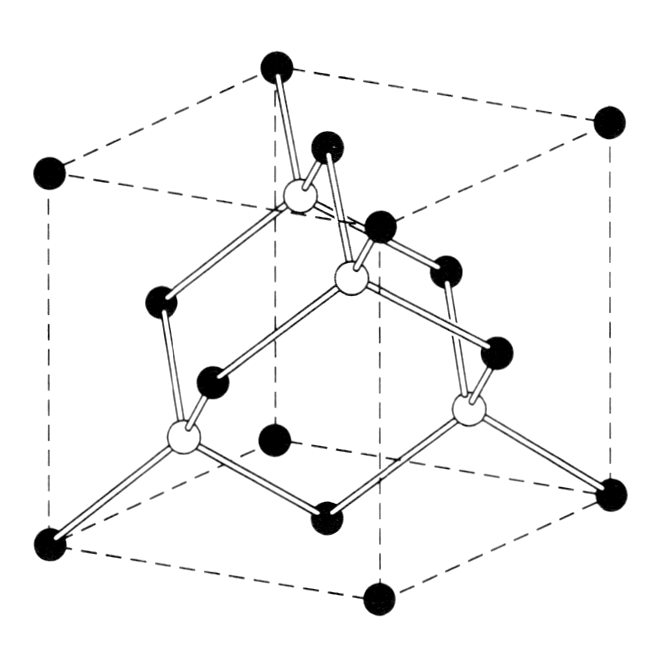
\includegraphics[width=.9\linewidth]{andere_bilder/diamond.png}
		\end{minipage}
		\hfill
		\begin{minipage}[c]{.25\linewidth}
			\centering
			\begin{tabular}{c c c c} 
				\hline
				& \textbf{x} & \textbf{y} & \textbf{z}\\ 
				\hline 
				\vspace{0.2cm} 
				$\fata_1$ & 0 & $\frac{a}{2}$ & $\frac{a}{2}$ \\
				\vspace{0.2cm}
				$\fata_2$ & $\frac{a}{2}$ & 0 & $\frac{a}{2}$ \\
				\vspace{0.2cm}
				$\fata_3$ & $\frac{a}{2}$ & $\frac{a}{2}$ & 0 
			\end{tabular}	
		\end{minipage}
		\hfill
		\begin{minipage}[c]{.33\linewidth}
%			\textbf{fcc}
%			\begin{tabular}{c c c c} 
%				\hline
%				& \textbf{x} & \textbf{y} & \textbf{z}\\ 
%				\hline 
%				\vspace{0.2cm} 
%				basis atom & 0 & 0 & 0 \\
%			\end{tabular}	
%			\vfill
%			\textbf{diamond} 
			\begin{tabular}{c c c c} 
				\hline
				& \textbf{x} & \textbf{y} & \textbf{z}\\ 
				\hline 
				\vspace{0.2cm}
				basis atom & 0 & 0 & 0 \\
				\vspace{0.2cm}
				basis atom & $\frac{a}{4}$ & $\frac{a}{4}$ & $\frac{a}{4}$
			\end{tabular}	
		\end{minipage}
		\caption{This is the cubic diamond lattice on the left (Picture from\cite{Kittel}). In the middle there are the basis lattice vectors of the primitive unit cell for a diamond crystal, and on the right there are the basis atoms for fcc and diamond.
%		As one can see, the diamond structure just has an additional atom at $\frac{a}{4},\frac{a}{4},\frac{a}{4}$ as basis.
		}\label{fcc}
	\end{figure}
%	 On the other hand, the zinc blende structure, which HgTe is growing in, is nearly the same as the diamond structure, with the only difference namely that the basis atoms are of a different kind. In figure \ref{hgte_diamond001} is a picture of this lattice. The grey atoms are at the same place as the black ones in figure \ref{fcc}.	
%	-millersche indizes

%	It is important to know, onto which plane in a crystal one is looking while doing experiments. 
	\begin{figure}[tbp]
		\centering
		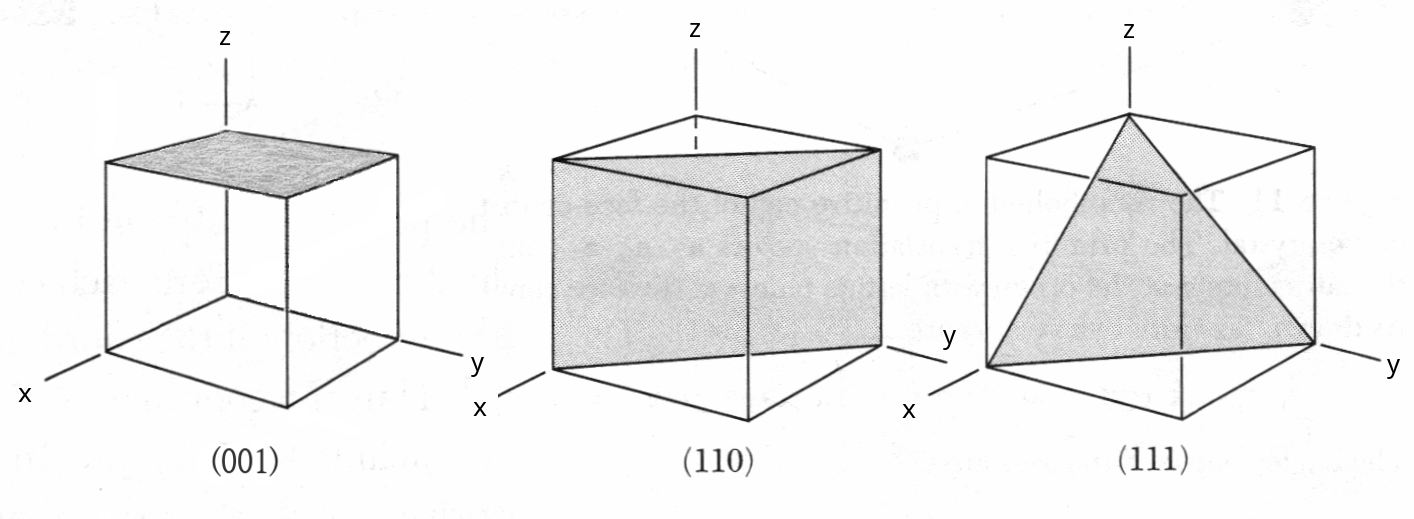
\includegraphics[width=.8\linewidth]{andere_bilder/millersche_indizes_less.png}
		\caption{Important planes in cubic crystals with their indices. At the left, there is the (001) which is analyzed for HgTe zinc blende structure in this thesis. (Picture from\cite{Kittel})} \label{millersche_indizes}
	\end{figure}
	Crystals are grown plane by plane in different directions. 
	Those planes can be identified by the so called miller indices ($hkl$).
%	These numbers are obtained by taking the reciprocal of the integers, with which one has to multiply the basis vectors, so that they are intercepting with the plane, and find the smallest integers for which the fractions have the same ratio.
	The integers $h$, $k$ and $l$ are obtained by multiplying each basis vector with a number, so that it touches the plane, inverting these numbers $x$, $y$ and $z$ in respect to multiplication, in other words, writing them in a fractions denominator, whereby these fractions are in the same ratio as the miller indices, and finally expand the fractions until they are integers indivisible by another integer. The connection between the miller indices and the numbers $x$, $y$ and $z$ is
	\begin{equation}
		h : k : l = \frac{1}{x} : \frac{1}{y} : \frac{1}{z}
	\end{equation}
	Some examples can be seen in figure \ref{millersche_indizes}.

	\begin{figure}[tbp]
		\begin{minipage}[c]{.32\linewidth}
			\centering
			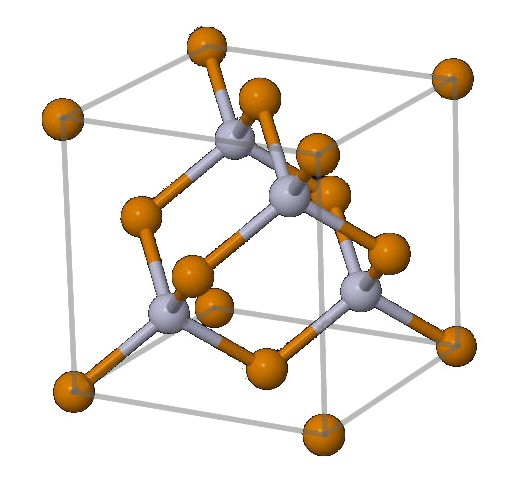
\includegraphics[width=0.9\linewidth]{andere_bilder/zinc_blende.jpg}
		\end{minipage}
		\hfill
		\begin{minipage}[c]{.32\linewidth}
			\centering
			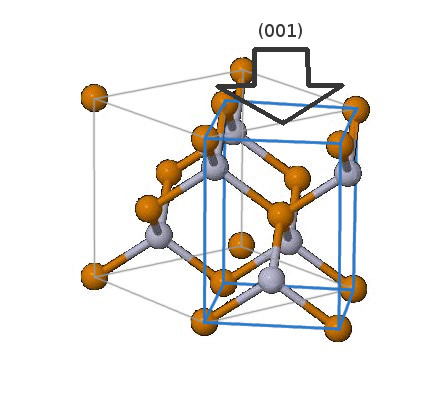
\includegraphics[width=\linewidth]{andere_bilder/zinc_blende_45degree.jpg}
		\end{minipage}
		\hfill
		\begin{minipage}[c]{.32\linewidth}
			\centering
			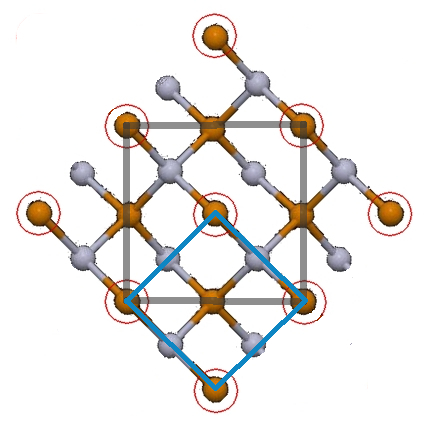
\includegraphics[width=.9\linewidth]{andere_bilder/001_plane_2.jpg}
		\end{minipage}
		\caption{Left: zinc blende structure, two different kinds of atoms are labeled as Te (orange) and Hg (grey), note that this is not a primitive unit cell. Middle: rotation of basis by $45^\circ$, so that the new unit cell is the blue cuboid. Right: the top view. The red circles mark the atoms at the top, the blue lines are the small cell with length $\frac{a}{\sqrt{2}}$. The grey large square represents the (001) plane of the old unit cell.} \label{hgte_diamond001}
	\end{figure}
%	-zinkblendestruktur
	
	In this thesis we will focus on the study of mercury telluride which is a crystal with two basis atoms Hg and Te, arranged in a zinc-blende structure. 
	In order to perform the calculations, we are focusing on HgTe at the diamond (001) cleavage, which is the top plane illustrated in figure \ref{millersche_indizes}. It is convention not to use the unit cell in the left of figure \ref{hgte_diamond001}, but to rotate the basis by $45^{\circ}$, like on the right. This has the advantage, that the unit cell contains less atoms. 
	%which means less computational effort. \marginpar{cite misses}
	
	The lattice vectors for diamond(001) are given by
	\begin{align} \label{001_basis}
		\fata_1&=\frac{a}{\sqrt{2}} \hat{\textbf{x}}; &
		\fata_2&=\frac{a}{\sqrt{2}} \hat{\textbf{y}}; &
		\fata_3&=a \hat{\textbf{z}}
	\end{align}
	where $a$ is the lattice constant of the crystal \cite{Graz} illustrated in the to the right in figure \ref{hgte_diamond001}. 
%	Later I will not use just $a$ for the z-direction, but $L$ which is composed of the slab thickness and the vacuum thickness on top of the surface. 
	In our case the basis atoms are at
	\\
	\begin{center}
		\begin{tabular}{c c c c} 
			\hline
			& \textbf{x} & \textbf{y} & \textbf{z}\\ 
			\hline 
			\vspace{0.2cm} 
			atomic species 1 & 0 & 0 & 0 \\
			\vspace{0.2cm}
			atomic species 2 & $\frac{a}{2\sqrt{2}}$ & 0 & $\frac{a}{4}$ \\
			\vspace{0.2cm}
			atomic species 1 & $\frac{a}{2\sqrt{2}}$ & $\frac{a}{2\sqrt{2}}$ & $\frac{a}{2}$ \\
			\vspace{0.2cm}
			atomic species 2 & 0 & $\frac{a}{2\sqrt{2}}$ & $\frac{3a}{4}$
		\end{tabular}
	\end{center}	
%	-reziproker raum
%	-Brillouin zonen
%	-band structure
	\FloatBarrier
	\subsubsection{Reciprocal lattice and first Brillouin zone.} \label{Brillouin_zone}
	\begin{figure}[t!]
		\centering
		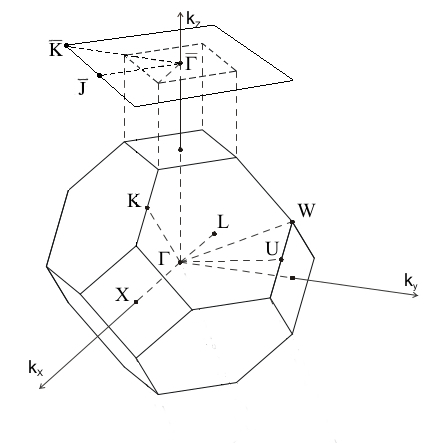
\includegraphics[width=.5\linewidth]{andere_bilder/brillouin_zone_001_2.jpg}
		\caption{First Brillouin zone of a fcc and diamond lattice. 
%		In addition, there is the (001) plane at the top, which is a 2D Brillouin zone. The super symmetric points are marked with Latin letters and the one in the center with a $\Gamma$. 
		The plane at the top shows the 3D Brillouin zone projected in (001) direction, which is also defined by the vector $\boldsymbol{b}_3$. This corresponds to the first Brillouin zone in the 2D lattice. The high symmetry point are marked with latin letters, whereby the ones in the two dimensional Brillouin zone additionally have a bar and the point of origin is marked with a $\Gamma$, a bar is added for the one in the 2D Brillouin zone.  
%		The points at the plane are additionally marked with a bar to distinguish them from the 3D Brillouin zone's points. 
		(Picture originally from\cite{aluminium})}\label{brillouin_zone}
	\end{figure}
%		The reciprocal lattice of a Bravais lattice is the set of all wave vectors $\K$, which is produced by plane waves together with the periodicity of a given Bravais lattice.  
%		The relation between the vectors $\R$, which describe the given Bravais lattice, and the wave vectors $\K$ is
		The reciprocal lattice is defined as the Fourier transform of the direct Bravais lattice in real space. This transformation is mathematically equivalent to
		\begin{equation} \label{exp}
		e^{i \K \cdot \R} = 1.
		\end{equation}
		where $\K$ is the set of wave vectors in reciprocal space and $\R$ is defined as in Eq. \ref{vector}.
		Consequently, every direct lattice has a corresponding reciprocal lattice which in addition, is a Bravais lattice too, since the Fourier transform acts within a group of discrete symmetries.		
%		A reciprocal lattice is only defined in respect to its Bravais lattice. The consequence is, that the reciprocal lattice is a Bravais lattice itself. Its vectors can generally be defined as:
		The primitive translation vectors of the reciprocal lattice can be obtained from Eq. \ref{exp} and their basis vectors are in three dimensional space related to the direct lattice vectors as
		\begin{align}
			\bb_1 &= \frac{2\pi}{V}(\fata_2 \times \fata_3); &
			\bb_2 &= \frac{2\pi}{V}(\fata_3 \times \fata_1); &
			\bb_3 &= \frac{2\pi}{V}(\fata_1 \times \fata_2)
		\end{align} 
		with $V=\fata_1 \cdot \fata_2 \times \fata_3$ being the volume of the primitive unit cell in real space.
		 
		The primitive Wigner-Seitz cell in the reciprocal space is called the first Brillouin zone. 
%		It is constructed similar and it has so called super symmetric points.
		The principle of constructing the first Brillouin zone is the same as for the earlier described Wigner-Seitz cells construction. The points, who stand out as high-symmetry points of the Brillouin zone, are marked by letters like K, L, U etc. The center of the Brillouin zone which happens to also be the origin of the Fourier space, is marked with the greek letter $\Gamma$.  
		The first Brillouin zone of the fcc and diamond crystal is shown in figure  \ref{brillouin_zone}.		
%		Since the zinc-blende structure is important for this thesis, it is good to know, that the reciprocal vectors of an fcc lattice are the primitive vectors of a bcc lattice but with a different length:

%		\begin{align} \label{fcc_reciprocal_vectors}
%			\bb_1 &= \frac{2\sqrt{2}\pi}{a} \hat{\textbf{x}} ;&
%			\bb_2 &= \frac{2\sqrt{2}\pi}{a} \hat{\textbf{y}} ;&
%			\bb_3 &= \frac{2\pi}{a} \hat{\textbf{z}}	
%		\end{align}

%	\begin{figure}[tbp]
%		\centering
%		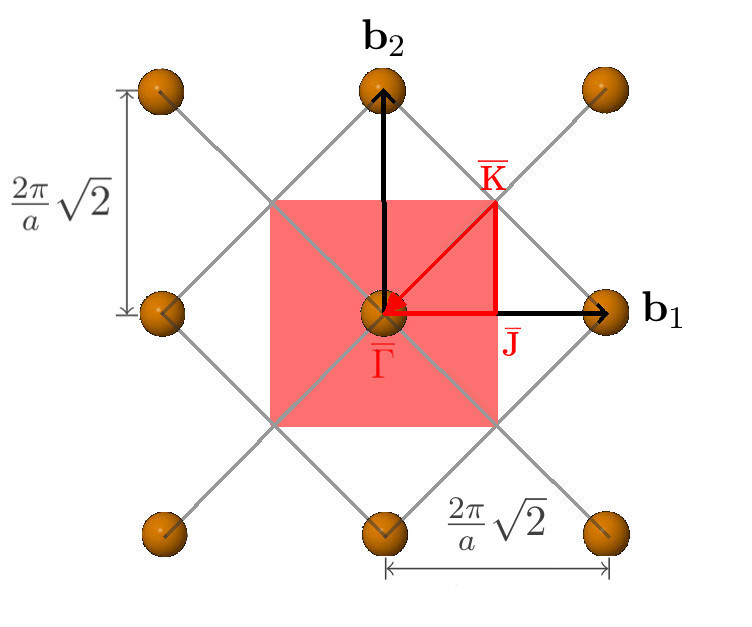
\includegraphics[width=.5\linewidth]{001_reciprocal_plane.jpg}
%		\caption{The light red region is the first Brillouin zone. The red line is the \textbf{k}-path for obtaining the band structure by calculating the dispersion relation. (Picture like in \cite{Graz})}\label{brillouin_zone_001}
%	\end{figure}
%		For calculating band structure of the bulk, one has to go a certain path along the symmetric points. 
%		But, in order to calculate the surface states of the HgTe, one has to choose which cleavage should be regarded. This also means $\Gamma$, X, L etc. of the 3D Brillouin zone cannot be used. Instead the super symmetric points of the 2D Brillouin zone must be taken. For the (001) plane those \textbf{k}-points, which are also illustrated in figure \ref{brillouin_zone_001},  are:
		
		The bulk band structure (see figure \ref{bulk_band_structure}), which gives the total energy in respect to the momentum, can now be seen as a one dimensional representation of a certain path which follows the high-symmetry points in the first Brillouin zone. 
		
		For the 2D periodic crystal slab, which grows in (001) direction, a two dimensional path can be taken along the high-symmetry points $\overline{\Gamma}$, $\overline{\text{J}}$ and $\overline{\text{K}}$. These points can be represented in terms of the reciprocal vectors $\bb_1$ and $\bb_2$:
		\begin{align} \label{2D-BZ-points}
			\overline{\Gamma}&= 0;&
			\overline{\text{J}} &= \frac{1}{2} \bb_1 ;&
			\overline{\text{K}}&= \frac{1}{2} \bb_1 + \frac{1}{2} \bb_2 
		\end{align}
		Therefore the 2D Brillouin zone, which corresponds to the slab, is like the projection of the 3D Brillouin zone into a plane which is defined by the vector $\bb_3$. 
		
%		in respect to the reciprocal basis vectors \eqref{fcc_reciprocal_vectors}. 
%		For calculating the dispersion relation $E(k)$ of this plane, one has to go the along the red line in figure \ref{brillouin_zone_001}.
	%	-surfaces
	\subsubsection{Surface modeling} \label{surface_modeling}
%		In order to perform calculations for the surface states and properties, there are certain points about how to model the surface conditions correctly for getting physically correct results. Beginning with the boundary conditions, the bulk has 
%%		The way of calculating the dispersion relation was already explained in \ref{Brillouin_zone}, but after knowing the crystal and surface structure of HgTe in \ref{cleavage_fcc} I still didn't discuss how to exactly simulate the surface and the bulk.  
%%		
%%		The boundary conditions for the bulk are
%		infinite repetition in all three space directions. 
%		
%		In contrast, the surface has infinite repetition in two directions, here where the (001) plane is normal to the z-direction, thats the boundary condition in x- and y-direction for the surface calculations. But in the z-direction, thus the third direction, there is no repetition.
		The main goal of this thesis is to simulate the evolution of the topological surface states of HgTe. Therefore we first need to introduce the concept of surfaces and then simulate the (001) surface for an ideal slab. 
		
		The bulk is a model of a crystal which does not consider surfaces. For us, the most important difference are the boundary conditions. The bulk has periodic boundary conditions in all three spacial directions, but the slab, has these in just two directions, in particular the x and y direction. Thus $k_z$ is no longer a good quantum number.  How this direction is simulated is explained in the following paragraphs. 
%		the termination of the crystal must be simulated. 
	\paragraph{Terminations}
	\begin{wrapfigure}{r}{0.3\linewidth}
		\centering
		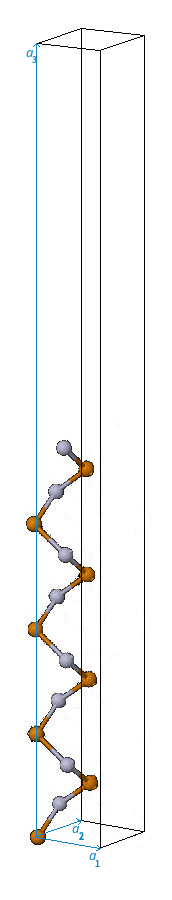
\includegraphics[width=0.6\linewidth]{andere_bilder/hgte_16layer_supercell_2.jpg}
		\caption{Supercell with 16 layers and additional space at the top, representing the vacuum. Basis vectors $\fata_1$, $\fata_2$ like in eq. \ref{001_basis}, $\fata_3$ with additional vacuum thickness.} \label{16layer_supercell}
		\vspace{-1cm}
	\end{wrapfigure} 	
%		One has to regard two surfaces at the bottom and at the top of the crystal in z-direction, which means it can be terminated by the same atoms, Te or Hg at the bottom and at the top, or it can be terminated by two different atoms, for example Te at the bottom, Hg at the top.
%		The first possibility is symmetric, while the latter is asymmetric. 
%		
%%		Even when the asymmetric slab can induce a dipole moment, it consists of an integer number of unit cells, which means it is stoichiometric. The dipole moment is here prevented by Hydrogens at the bottom surface. Those Hydrogens saturate the dangling bonds of tellurium (still have no clue why I used them by reading ???????)
%		In this thesis I will compare those terminations with the same ones but with additional hydrogens at the bottom, which is a more realistic simulation for the surface. The reason is that HgTe would rather be terminated by Te and Hg mixed surfaces than smooth ones. Since this is very difficult for FHI-aims to simulate, this is the alternative. 
		
		While simulating the slab, one must consider two surfaces which are both terminated with atoms. Thereby it is very difficult to find a way to prevent interactions between the surfaces. In a real simulation this is done by passivating one surface for example by adding hydrogen atoms, in order to get a neutral surface. These hydrogens saturate the dangling bonds, the unsatisfied valences on immobilized atoms.
		
		During this work, we study diverse possible terminations. On the one hand it is the symmetrical case with Hg-Hg and Te-Te as termination on both surface, on the other hand, we regard the antisymmetrical case with Te-Hg termination, whereby also both versions, with and without passivation with hydrogen, are studied. 
%		, so that the conduction band is lowered, which means the electrons can flow better on the surface.
	\paragraph{Number of layers}
		As mentioned before, the main goal of this thesis is the investigation of the topological surface states' evolution by adding layers in one growth direction. Discussing the number of layers is therefore essential. The termination defines whether the number of layers is even or odd. For the slabs with same atom termination the number of layers is odd and for the ones with different atom termination it is even. 
		
		For each one we took 3 different numbers of layers in order to simulate the growth of a mercury telluride crystal in the (001) plane, observing at which thickness the surface states presents characteristics of those of a topological insulator. One layer is defined as one of five layers in the crystal unit cell in figure \ref{hgte_diamond001}, in other words, for your coordination choice all atoms with the same z-component are in the same layer.
		 
	\paragraph{The Supercell Approach}
		For simulating the surface structure of a crystal, the so-called supercell approach might be useful. The concept is rather simple. First one constructs the unit cell for the slabs, which will be duplicated infinite times in all directions. Since $k_z$ is a bad quantum number, the repetition in z-direction presents a problem. But FHI-aims can only solve the Schrödinger equation with periodic boundary condition applied in all three directions. This means, that in x and y direction, the lattice is repeated into infinity but, also the the slabs from an infinite stack into the z-direction.
		To prevent interactions between the surfaces, we add a sufficiently large vacuum slab to the supercell which makes sure that the slabs can be regarded as isolated. 
%		to multiply the unit cell into the direction of the surface which is, if the coordinates are chosen wisely, the z-direction. Additionally there has to be a large space added which represents the vacuum space on top of the surface.
		A supercell of 16 layers of HgTe is shown in figure \ref{16layer_supercell}.
	
%		The boundary conditions for the other two directions which is infinite repetition, is provided by an integration in the \textbf{k}-space. In FHI-aims the integration points can be set by the k-grid command,
%		\begin{verbatim}
%			k_grid 12 12 1
%		\end{verbatim}
%		where the three numbers are the number of points in x, y and z direction.
%	\subsubsection{Band structure}

		%%% Local Variables:
		%%% mode: latex
		%%% TeX-master: "main_BA2.0"
		%%% End:
	
	\subsection{Basics of Density Functional Theory}
		%The density functional theory (DFT)
	%(What is it? Who discovered DFT? Functionals ) and mention code packages used for the study of band structures.
	The density functional theory (DFT) is a computational method in quantum mechanics used for analyzing the ground state properties of physical systems. 
	Ab-initio stands for calculations which are performed only by using fundamental laws of physics like the Schrödinger equation for quantum mechanical problems. At the same time, no approximations are taken whereby symmetries are still included. Consequently, one usually needs notable large computational resources.
%	ab inito calculation method for the dispersion relation. Ab-initio is Latin and means 'from the beginning'. These kinds of calculations are based on well established and basic laws of physics and no additional assumptions or special models are used. In solid state physics, the methods of calculating the properties of solids are often based on approximations and are not consider every atom's influences. But the ab-initio calculation method does. The consequences are, that there is a huge amount of CPU effort in need, even for small input.
	The DFT was first introduced by W.Kohn et al. \cite{Kohn}. Thereby it was found that the ground-state energy of a quantum mechanical system can be represented by the density functional. This simplifies the many-body problem down to a self-consistent one-body problem.  
	
	In the following most equations were adapted from \cite{solid_state_book}
%	The DFT was first introduced by the Thomas-Fermi model 1927 \cite{Graz}, but this model gave poor results. It took 30 years till Hohenberg and Kohn developed their energy functional which was then upgraded by Kohn and Sham.
	\subsubsection{The ground-state functional}
%	It is shown by the DFT, that instead of searching for ground-state of a many-electron wavefunction, the ground-state one-body electron density $\rho(\textbf{r})$ can be used.  
	
	Let us consider a system containing $N$ electrons 
%	and the standard many-electron
	with Hamiltonian $H_e$ 
%	which consists of the inner part with kinetic energy $T$ and the electron-electron Coulomb interactions $V_{\text{ee}}$, and of the external potential, which is in this case the interaction between the nuclei and the electrons. 
	that contains three parts: kinetic energy $T$, external potential $V_{ext}$, which describes the interaction between the electrons and a fixed nuclei background, and the two-body electron-electron interaction known as the Coulomb potential $V_{ee}$.
	\begin{align}
		H_\text{e} = T + V_{\text{ee}} + V_{\text{ext}} &= \sum_i \frac{\textbf{p}^2_i}{2m} +
		\frac{1}{2} \sum_{i\neq j} \frac{e^2}{|\rr_i - \rr_j|} + \sum_i v_{\text{ext}}(\rr_i) \\
		\text{with} ~v_{\text{ext}}(\rr) &= V_{\text{nucl}}(\rr)= -\sum_I \frac{z_I e^2}{|\rr - \R_I|}
	\end{align}	
	where $e$ is the elementary charge.
	The external potential $V_{ext}$ contains the interaction between each proton $I$ in the nuclei whereby $z_I$ is the number of all protons in the nuclei, and each electron $i$, $v_{ext}(\rr)$ is therefore the external potential for a single electron in the potential background of a nuclei. 
%	The ground-state $\Psi_\text{G}(\rr_1,\dots,\rr_N)$ of many electrons just depends on the external potential $v_{\text{ext}}(\rr)$. And the one-body ground-state density $\rho(\rr)$ can be defined as 

	If $\Psi_G(\rr_1,\dots,\rr_N)$ is the wave function of the ground state in the many body Schrödinger equation
	\begin{equation}
		H_e \Psi_G = E_G \Psi_G
	\end{equation}
	then it can be shown, that the one-body ground states density, which is defined as
	\begin{equation}
		 \rho(\rr) = \braket{\Psi_\text{G}(\rr_1,\dots,\rr_N)|\sum_i \delta (\rr -\rr_i)| \Psi_\text{G}(\rr_1,\dots,\rr_N)}
	\end{equation}
	can be uniquely converted into the external Potential $V_{ext}(\rr)$ and vice versa. In other words, for one given $V_{ext}(\rr)$ there exists specifically one $\rho(\rr)$. This is known as one of the Hohnberg-Kohn theorems \cite{solid_state_book}. 
%	which leads to
%	\begin{equation}
%		\braket{\Psi_\text{G}|V_{\text{ext}}| \Psi_\text{G}} =
%		\int \rho(\rr) v_{\text{ext}}(\rr) \diff \rr.
%	\end{equation}
%	This means, there is a functional that links $\rho(\rr)$ and $v_{\text{ext}}(\rr)$ and if there are several different $v_{\text{ext}}$, then they correspond to different ground-state density functions.
	
	The second Hohenberg-Kohn theorem says that the ground state energy can be expressed in a density functional. That functional is called the Hohenberg-Kohn energy functional (\cite{solid_state_book} p.133) and reads
%	The useful result of this theorem is the knowledge, that the ground-state energy is a functional $E[\rho]$ containing the expectation values of the kinetic energy an the electron-electron interaction. It is called the Hohenberg-Kohn energy functional 
	\begin{equation} \label{HK_functional}
		E^{\text{HK}}[\rho(\rr);v_{\text{ext}}(\rr)] = 
		T[\rho(\rr)] + V_{\text{ee}}[\rho(\rr)] + \int v_{\text{ext}}(\rr) \rho(\rr) \diff \rr 
	\end{equation}
%	The ground-state is found by minimizing $E^{HK}$, and the density $\rho_0$ which minimizes it, is the ground-state density.
	This means now the ground-state energy of a many-body problem can be disposed immediately if the density is known. 

	By rearranging the functional above, we define the so-called exchange-correlation functional $E_{xc}[\rho]$:
	\begin{align}
	E_{xc}[\rho] = T[\rho] - T_0 [\rho] + V_{\text{ee}} [\rho] - V_\text{H} [\rho]
	\end{align}
	so that equation \eqref{HK_functional} is now
	\begin{equation}
	E^{\text{HK}}[\rho(\rr); v_{\text{ext}}(\rr)] = 
	T_0 [\rho] + V^\text{HK}(\rr)
	\end{equation}
	with the kinetic energy of a system with non-interacting electrons:
	\begin{equation}
		T_0 [\rho] = \sum_i \braket{\phi_i(\rr)| -\frac{\hbar^2 \nabla^2}{2m} | \phi_i(\rr)}
	\end{equation}  
	and the Hohenberg-Kohn potential
	\begin{equation}
		V^\text{HK}(\rr)= V_\text{H} [\rho] + \int v_{\text{ext}}(\rr) \rho(\rr) \diff \rr + E_{\text{xc}} [\rho]
	\end{equation}
	with the Hartree potential which is defined as
	\begin{equation}
		V_\text{H}[\rho]= \frac{1}{2} \sum_{i,j} \braket{\phi_i \phi_j| \frac{e^2}{|\rr_i-\rr_j|} |\phi_i \phi_j}.
	\end{equation}
	
	Until now, we didn't get anything useful. However the original problem was cleverly rewritten in a way, that the minimization of $E^\text{KH}$ produces the so-called Kohn-Sham equations. These are the effective one-particle equations which are Schrödinger-like. Their eigenfunctions are called Kohn-Sham orbitals $\phi_i(\rr)$ which depend on the particle density $\rho(\rr) = \sum_i |\phi_i(\rr)|^2$.
%	Now , the Kohn-Sham equations are minimizing the functional in respect do $\rho(\rr)$, by bringing it into the form $ \rho(\rr) = \sum_i \phi_i^*(\rr) \phi_i(\rr) $ while the wave functions are orthonormalised. 

	
	The solution of the Kohn-Sham equation gives rise to the total ground state energy as 
%	The Kohn-Sham equations are evaluated by variating the exchange-correlation functional. This will give us a ground-state functional which looks like this
	\begin{equation} \label{ground-state_functional}
		E_0 [\rho_0] = E_{\text{nucl}} + E_{\text{kin}} + E_\text{H} + E_{\text{xc}} 
	\end{equation}
	including the potential of the electron-nuclei interaction, the kinetic energy, the Hartree potential and the exchange-correlation functional.
	
	\subsubsection{Approximations for the exchange-correlation functional} \label{xc-func}
%		The last one in equation \eqref{ground-state_functional} must be approximate while the other parts can be well calculated.
		In contrast to the other functionals on the left side in eq. \eqref{ground-state_functional}, the exchange-correlation part is not known exactly, thus one has to think about some approximation schemas.
		There are different kinds, the simplest one is the local density approximation (LDA) where 
		\begin{equation}
		E_{\text{xc}}^{\text{LDA}}[\rho] = \int \epsilon_{\text{xc}} (\rho(\rr)) \rho(\rr) \diff \rr
		\end{equation} 
		with the many-body exchange-correlation energy per electron $\epsilon_{xc}(\rho)$ of a uniform gas with density $\rho(\rr)$ of interacting electrons.
		
		In this thesis the Perdew-Burke-Ernzerhof (PBE) functional which is a generalized gradient approximation (GGA) has been used. It is a semilocal-density functional, which is not only dependent on the density at a position $\rr$. This functional is better for big molecules or systems.
%		which means in comparison with LDA, it is better for big molecules or systems with more atoms. The PBE functional fulfills many of the physical and mathematical requirements of the DFT but is unsatisfactory for total energies of molecular systems \cite{PBE}.
		
		It is of the form:
		\begin{equation}
			E_{\text{xc}}^{\text{PBE}} = \int \diff^3 r \rho(\rr) 
			\,\epsilon_{\text{xc}}^{\text{PBE}} (r_s (\rr), s(\rr), \zeta(\rr))
		\end{equation}
		where $r_s$ is the Wigner-Seitz radius, $\zeta$ is the spin polarization and the reduced density gradient $s=\frac{|\nabla \rho|}{2 k_F \rho}$ with $k_F = (3 \pi^2 \rho)^{\frac{1}{3}}$. 
%%% Local Variables:
%%% mode: latex
%%% TeX-master: "main_BA2.0"
%%% End:
	
	\subsection{Spin-orbit coupling} \label{chapter_soc}
		This subsection follows the content of \cite{tutorial2} appendix 4,5 and 6. 
%In this subsection it is explained which Schrödinger equation FHI-aims uses by including some keywords, in order to incorporate relativistic effects. 

\subsubsection{Spin-orbit coupling in Schrödinger equation}
	
%	FHI-aims considers relativistic effects, if one includes the atomic ZORA where the scalar energy is set to zero and only the free-atom potential of the nearest atom is used.
%	The formal equation is a scalar-relativistic Schrödinger equation which can be written as \cite{tutorial2}
%	\begin{equation} \label{scalar-relativistic_Schroe}
%		\left(
%			\p \frac{c^2}{2 c^2 + \epsilon - V} \p + V
%		\right) \Psi = \epsilon \Psi
%	\end{equation}
%	with rescaled kinetic energy. 
	The spin-orbit interaction is the mutual interaction between a particles spin and its motion. 
	The Dirac-equation for electrons \eqref{Dirac_equation} explaines why this type of coupling should be included in the Schrödinger equation, or rather the Pauli equation, since we are including the additional spin structure by two spinors: 
%	The spin-orbit coupling is links the spin and the momentum of a particle. For the calculations an equation which includes the spin is needed.
%	Since the Schrödinger equation %\ref{scalar-relativistic_Schroe} 
%	does not consider the spin,	an other equation needs to be regarded: The Dirac-equation:
	\begin{equation} \label{Dirac_equation}
		\left(
			c \boldsymbol\alpha \cdot \p + c^2(\beta - 1) + V) 
		\right) \Psi = \epsilon \Psi
	\end{equation}
%	which is a relativistic four-dimensional equation. It is modeling electrons and positrons in a superposition state $\Psi$ with the Dirac matrices 
	where $\Psi$ is a four-dimensional wave function whereas $\boldsymbol{\alpha}$ and $\beta$ are the $4 \times 4$ matrices
	\begin{align}
		\boldsymbol\alpha &= 
		\begin{pmatrix}
			0 & \boldsymbol{\sigma} \\
			\boldsymbol{\sigma} & 0
		\end{pmatrix} & &\text{and} &
		\beta &= 
		\begin{pmatrix}
		\mathds{1}_2 & 0 \\
		0 & -\mathds{1}_2
		\end{pmatrix}
	\end{align}
%	which are acting on the four-dimensional spinor $\Psi$ including the Pauli matrices
	with $\boldsymbol{\sigma} = (\sigma_x, \sigma_y, \sigma_z)$:
	\begin{align}
		\sigma_x &=
		 \begin{pmatrix}
		 0 & 1 \\
		 1 & 0
		 \end{pmatrix} ,&
		 \sigma_y &=
		 \begin{pmatrix}
		 0 & -i \\
		 i & 0
		 \end{pmatrix} ,&
		 \sigma_z &=
		 \begin{pmatrix}
		 1 & 0 \\
		 0 & -1
		 \end{pmatrix}.
	\end{align}
	which are the Pauli matrices. The term $\boldsymbol{\alpha} \cdot \p$ explicitly shows the coupling of spin and momentum, since it includes a momentum operator, which acts on the orbital wave function, and the matrix $\boldsymbol{\alpha}$, which is acting on the spin degrees of freedom.
%	For getting the full potential is normally in need of quantum-electrodynamic treatment, but for quantum chemistry and condensed matter physics, this can be cut down to the Coulomb and Breit terms \cite{tutorial2} where the latter will not be regarded further in this case because it is neglectable.
%	
%	The solutions for electrons for \ref{Dirac_equation} are positive energies and are obtained by separating $\Psi$ into a two-dimensional large component $\Psi_L$ and a two-dimensional small component $\Psi_S$, where the first one corresponds to spin-up and spin-down electrons and the second to spin-up and -down positrons
	It is essential to solve the equation which includes the coupling of all $\Psi$ components. Fortunately in condensed matter systems it is possible to expand eq.\eqref{Dirac_equation} in terms of $\frac{v}{c}$ and get a simpler non-relativistic equation which is still quite precise.
	In order to do so, we separate $\Psi$ into two components, the 'larger' $\Psi_L$, which dominates for the non-relativistic limit, has positive energies and therefore represents the electron and the 'smaller' $\Psi_S$ component with negative energies and which represents a positron. 
	\begin{equation}
		\Psi = 
		\begin{pmatrix}
			\Psi_L \\ \Psi_S
		\end{pmatrix}
	\end{equation}	
	Substitution into Dirac equation \eqref{Dirac_equation}: 
	\begin{align}
		\left[
			c 
			\begin{pmatrix}
			0 & \boldsymbol{\sigma} \\
			\boldsymbol{\sigma} & 0 
			\end{pmatrix}
			\cdot \p
			+ c^2
			\left(
				\begin{pmatrix}
					\mathds{1}_2 & 0 \\
					0 & \mathds{1}_2
				\end{pmatrix} 
				- 1
			\right)
			+ V
		\right] 
		\begin{pmatrix}
			\Psi_L \\
			\Psi_S
		\end{pmatrix} 
		&= \epsilon 
		\begin{pmatrix}
			\Psi_L \\
			\Psi_S
		\end{pmatrix} \\	%nächste Zeile
		\Leftrightarrow ~~
		c
		\begin{pmatrix}
			\boldsymbol{\sigma} \cdot \p ~\Psi_S \\
			\boldsymbol{\sigma} \cdot \p ~\Psi_L
		\end{pmatrix}
		+
		c^2
		\begin{pmatrix}
			\Psi_L \\
			\Psi_S
		\end{pmatrix}
		+
		(-2c^2 +V)
		\begin{pmatrix}
			\Psi_L \\
			\Psi_S
		\end{pmatrix}
		&= \epsilon 
		\begin{pmatrix}
			\Psi_L \\
			\Psi_S
		\end{pmatrix} \\ %nächste Zeile
		\Leftrightarrow~~
		c
		\begin{pmatrix}
			\boldsymbol{\sigma} \cdot \p ~\Psi_S \\
			\boldsymbol{\sigma} \cdot \p ~\Psi_L
		\end{pmatrix}
		+
		\begin{pmatrix}
			V~\Psi_L \\
			(-2c^2+V)~\Psi_S
		\end{pmatrix}
		&= \epsilon 
		\begin{pmatrix}
			\Psi_L \\
			\Psi_S
		\end{pmatrix}
	\end{align}
yields two coupled equations 
	\begin{enumerate}[(i)]
		\item $c ~(\boldsymbol{\sigma} \cdot \p) ~\Psi_S + V~\Psi_L = \epsilon~\Psi_L	$ \label{1}
		\item $c ~(\boldsymbol{\sigma} \cdot \p) ~\Psi_L + (-2c^2+V)~\Psi_S = \epsilon~\Psi_S$ \label{2}
	\end{enumerate}
Transpose Eq.(\ref{2})
	\begin{align}
		((2c^2 - V) + \epsilon) \Psi_S &= c~(\boldsymbol{\sigma} \cdot \p)\Psi_L	\\
		\Leftrightarrow
		\Psi_S &= c 
		\left(
			\frac{1}{2c^2 - V + \epsilon} 
		\right) 
		(\boldsymbol{\sigma} \cdot \p)\Psi_L \\
		\Leftrightarrow
		\Psi_S &= \frac{1}{2c}
		\left(
		{1 + \frac{\epsilon - V}{2c^2}} 
		\right)^{-1} 
		(\boldsymbol{\sigma} \cdot \p)\Psi_L,
	\end{align}
then inserting into Eq. (\ref{1})
	\begin{align}
		c ~(\boldsymbol{\sigma} \cdot \p)
		\left[
			\frac{1}{2c}
			\left(
			{1 + \frac{\epsilon - V}{2c^2}} 
			\right)^{-1}
		\right]		
		(\boldsymbol{\sigma} \cdot \p)\Psi_L
		+ V \Psi_L 
		&= \epsilon \Psi_L
	\end{align}
and by finally using $(\boldsymbol{\sigma} \cdot \fata)(\boldsymbol{\sigma} \cdot \bb) =  (\fata \cdot \bb) + i (\fata \times \bb) \cdot \boldsymbol{\sigma} $ 
%and rewriting the part in squared bracket together with the $c$,
we obtain
	\begin{align} \label{SOC_equation}
		\left(
			\p \frac{c^2}{2c^2 + \epsilon - V} \p 
			+ i \p \frac{c^2}{2c^2 + \epsilon - V} \times \p \cdot \boldsymbol{\sigma} 
			+ V 
		\right) \Psi_L 
		&= \epsilon \Psi_L	
	\end{align}
	This equation is similar to the Schrödinger equation and is now quadratic in the momentum $\boldsymbol p$. For the scalar relativistic case, FHI-aims solves \eqref{SOC_equation} without including the second term. This term is corrected in respect to the kinetic energy and is called the \textit{scalar} relativistic Schrödinger equation. 
%This equation includes the Schrödinger equation in the relativistic case, which FHI-aims uses if one includes \texttt{relativistic} together with the atomic ZORA, but has no spin dependence. It is the first term together with the potential $V$, but regarded for $\epsilon = 0$ and in the free-atom potential of the nearest atom. 
	The well-known Schrödinger equation can be recovered by expanding eq. \eqref{SOC_equation} to lowest order in $(\epsilon - V)/2c^2$. Indeed,
%The non-relativistic case can be obtained by expanding \eqref{SOC_equation} in the zeroth order of $(\epsilon - V)/2c^2$, which in this case is nothing else like $c\rightarrow \infty$
	\begin{align}
		\frac{c^2}{2c^2 + \epsilon -V} = 
		\frac{1}{2}~ \frac{1}{1 + \frac{\epsilon-V}{2c^2}} 
	\end{align}
%and the last fraction is the geometric series $\frac{1}{1 + x}$, and if $x$ negligible then the geometric series is too. Additionally
	which equals $\frac{1}{2}$ for the zeroth order. The expansion of the first and second term is the same, but note that the crossproduct of these two identical vectors $\p \times \p$ is zero.
	This leads to the non-relativistic Schrödinger equation:
	\begin{align}
		\left(
		\frac{1}{2} \p^2 + V 
		\right)\Psi_L
		= \epsilon \Psi_L
	\end{align}

%The second term in \eqref{SOC_equation} is the spin-orbit coupling part. It can be evolved by expand it's Taylor series to lowest, not disappearing order in $x = (\epsilon - V)/2c^2$ where $\epsilon$ is also set to zero.
	Now let us consider the lowest non-trivial order of corrections coming from the second term in \eqref{SOC_equation} by using the Taylor series of the geometric series:
	\begin{align}
		f(x)=& \frac{1}{1+x} \\
		\text{Taylor series to first order:}& ~f(a) + \frac{f'(a)}{1!} (x-a)  \\
		\Rightarrow
		\frac{1}{1+a} + \frac{1}{2}
		\left(
			- \frac{1}{(1+a)^2}	
		\right)&
		(x - a) 
		\overset{a=0}{\underset{x=-V/2c^2}{=}}		
		1 + \frac{V}{2c^2}
	\end{align} 
%which means the first part is zero again, and the second yields
	By setting $\epsilon=0$ and looking for the non-trivial correction we obtain the spin-orbit interaction term  
	\begin{align}
		V_{SOC} = \frac{i}{4c^2} \p V \times \p \cdot \boldsymbol{\sigma}.
	\end{align}
	Relativistic effects don't need to be considered for structures with light atoms, if the electron is not near the nuclei. But if a structure contains heavy elements, like HgTe, it is necessary since spin-orbit also affects valence electrons.
%those effects no longer just occur near the nuclei. It additionally spreads out into the valence region. 

	Finally, we would like to point out that the actual calculation of FHI-aims, 
	is not considered self-consistently but is applied only after the self-consistent cycle of the density has converged.
%	the spin-orbit coupling is not included into the calculations of the band structure and energies, and is applied after the self-consistency circle converged. It is an perturbative method.

%For the calculations the keyword 
%	\begin{verbatim}
%		include_spin_orbit
%	\end{verbatim}
%must be set for activating the spin-orbit coupling calculations.
\subsubsection{SOC impact on band structure}
	The splitting behavior of the bands, which will be seen later in the results, is explained as follows.
	
	Beginning with the non-relativistic Schrödinger equation, the eigenstates with angular momentum $\ell$ and the spin $s$ can be written as a tensor product of a spatial function and a spin function, the spinor. For certain states, for example the s,p,d, etc. states for spherically symmetric potential, a particular symmetry of an external potential result in a particular banding of eigenvalues and symmetries between eigenvectors. 
%	This is known as the irreducible representations of the single group in group theory. 
	
	Adding the scalar-relativistic which brings us to the Schrödinger equation made out of the first part in \ref{SOC_equation} plus the $V$, the symmetry of the system doesn't change, but the Hamiltonian does. That means, that the eigenvalue of single electrons change, but the banding does not. 
	
	Turning on the spin-orbit coupling leads to a conservation of the total angular momentum $j=\ell + s$, but angular momentum and spin are no longer separately conserved. 
%	There are even no spin-up and spin-down eigenstates. Hence the single group symmetry, which was explained above, is broken. The Kramer's theorem explains that as long as time-reversal symmetry is conserved, the single electron states are double degenerated. 
	Consequently, the degeneracy in the spin quantum number might be lifted by the spin-orbit interaction and the bands might split (in some situations, some bands might still present accidental degeneracies)
	As a consequence, it is possible that the degeneracy in the spin quantum number is been reinforced by the spin-orbit coupling, so that the bands might split up. But note, that sometimes, some bands can still have coincidental degeneracies. 
%	This degeneracy leads to the band splitting due to the spin-$1/2$ character of the electron and the Zeeman effect which comes into account because of  the form of the SOC-operator.
	If the band splitting is very strong, some bands can even get inverted.
	
	
%%% Local Variables:
%%% mode: latex
%%% TeX-master: "main_BA2.0"
%%% End:
\section{Results}
	\subsection{Input for FHI-aims} \label{FHI-aims}
		All results were obtained by using FHI-aims \cite{aims}. 
	%Each calculation is been done in a separate folder.
	The input data are the files control.in and geometry.in.
	The geometry.in contains the lattice vectors' coordinates and the positions and types of the atom forming the basis. One example for the calculations of the bulk HgTe properties is:
		\begin{verbatim}
			# hgte lattice constant 6.685 AA
			lattice_vector	0.00000		3.34250		3.34250
			lattice_vector	3.34250		0.00000		3.34250
			lattice_vector	3.34250		3.34250		0.00000
			
			atom	0.00000		0.00000		0.00000 Te
			atom	1.67125		1.67125		1.67125 Hg
		\end{verbatim}
%	which is nothing else but the coordinates written in figure \ref{fcc}.
	
	The control.in contains all physical and computational settings for the calculation. The properties for the atoms also appear in the control.in, specifically the different types of basis sets settings.
%	are normally stored in the aims directory \texttt{SPECIES\_DEFAULTS} and have to be copied
	One can choose between \textit{light, tight} and \textit{really tight}, in this thesis we were using the \textit{light} settings.
%	But above that part, there are physical settings and the settings about the band structure output and the k-grid and about the convergence, for example for the k-grid study below:
	Among the setting one must consider the exchange-correlation functional, the spin, the numerical settings for the self-consistency cycle convergence and the grid size of the reciprocal lattice. For example see what we used for the bulk HgTe calculations:
	\\
	\begin{minipage}[c]{0.45\linewidth}	\vspace{15pt}
		\begin{verbatim}
		# Physical settings
		xc pbe
		spin none
		relativistic atomic_zora scalar
		default_initial_moment 0
		#
		\end{verbatim} 
	\end{minipage}
	\begin{minipage}[c]{0.55\linewidth} \vspace{11pt}
		\begin{verbatim}
		
		# method to be used, here pbe
		# spin treatment
		# include relativistic effects
		# initial spin for the atoms
		\end{verbatim}
	\end{minipage} 
	\begin{minipage}[c]{0.3\linewidth} \vspace{0.2cm}
		\begin{verbatim} 
			# SCF convergence
			sc_accuracy_rho		1E-4
			sc_accuracy_eev		1E-2
			sc_accuracy_etot		1E-5
			sc_iter_limit			100	
		\end{verbatim}
	\end{minipage} 
	\hfill
	\begin{minipage}[c]{0.7\linewidth} \vspace{0.15cm}
%		\vspace{8pt}
		\begin{verbatim}
		# convergence criteria of self convergence cycle
		# of change of density
		# of sum of orbital eigenvalues
		# total energy between two consecutive cycles
		# maximum of iterations
		\end{verbatim}
	\end{minipage} 
	\begin{minipage}[c]{0.3\linewidth}\vspace{0.2cm}
		\begin{verbatim}
			#
			# k_grid settings
			k_grid	8	8	8
		\end{verbatim}\vspace{8pt}
	\end{minipage}
	\hfill 
	\begin{minipage}[c]{0.7\linewidth}\vspace{28pt}
		\begin{verbatim}
		
		# k_x k_y k_z for the integration in k-space
		\end{verbatim}\vspace{8pt}
	\end{minipage} 

%	The spin was always set to none, otherwise, if it would be set to collinear, one would have to set \texttt{default\_initial\_moment} to \texttt{hund} or guessed it by hand.
	Spin none means that we deal with closed-shell calculations, in other words, the valence shell is regarded as filled \cite{closed_shell}. 
	The relativistic effects had to be taken into account since Hg and Te are both heavy elements and spin-orbit coupling, which is at the heart of the properties of topological insulators, can be considered as a low energy relativistic effect.
%	these effects, as explained in chapter \ref{topological_insulator}, are essential for the research of topological insulators.   
	
%%% Local Variables:
%%% mode: latex
%%% TeX-master: "main_BA2.0"
%%% End:
	
	\FloatBarrier
	\subsection{The lattice constant and the k-grid} \label{lattice_k-grid}
	\begin{figure}[ht!]
	\begin{minipage}{0.48\linewidth}
		\centering
		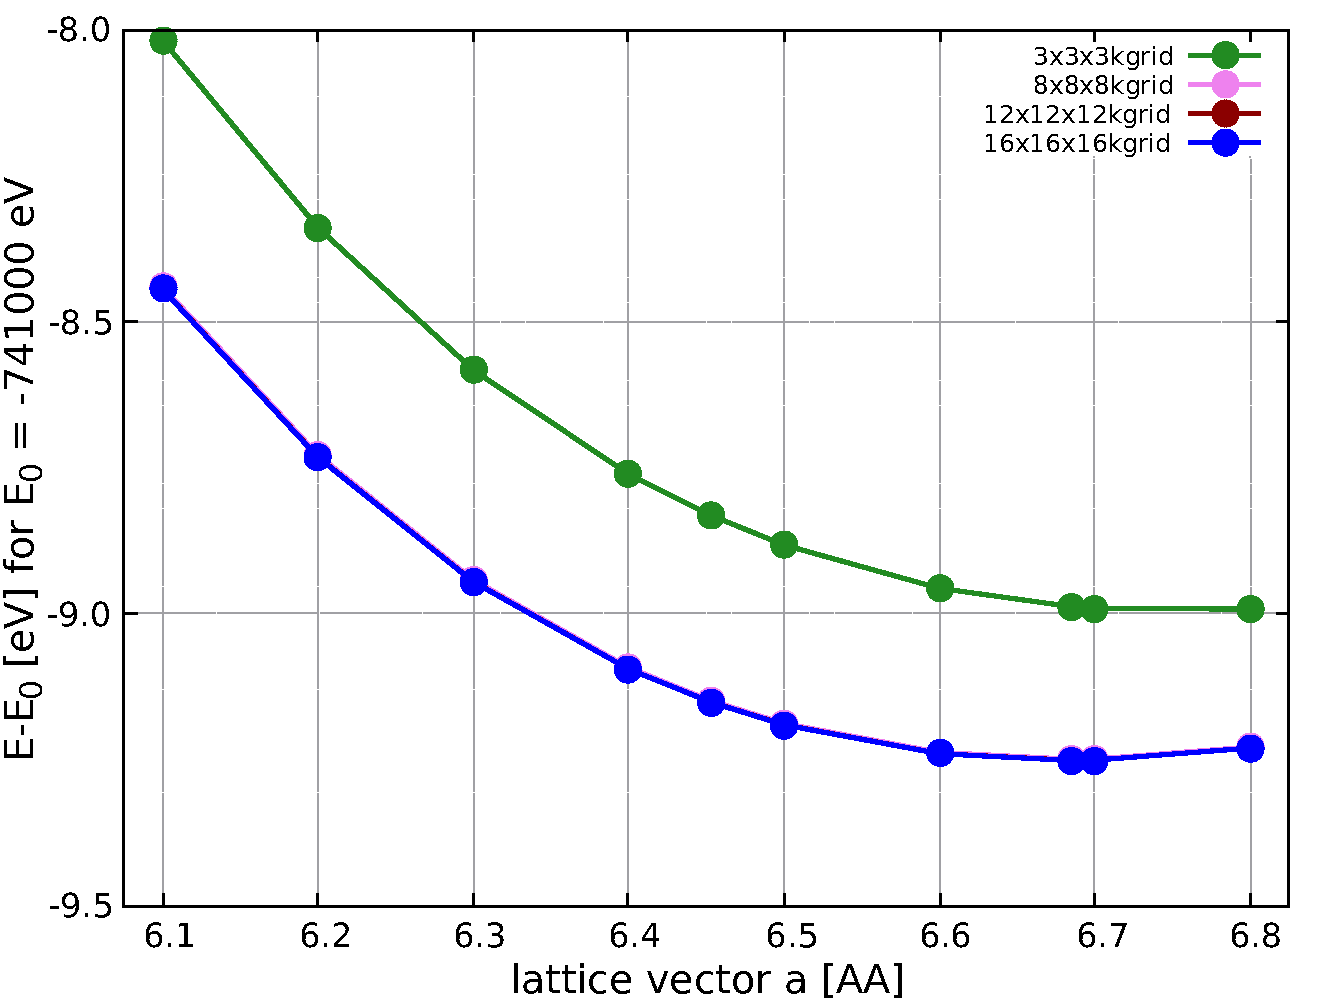
\includegraphics[width=\linewidth]{andere_bilder/plot_energies_hgte_bulk_all_kgrid_in_one.pdf}
		\caption{Lattice constant $a$ with respect to the total energy, calculated with four different k-grids. Lines for k-grids 8x8x8, 12x12x12 and 16x16x16 are overlaid.}\label{kgrid_lattice_constant}
	\end{minipage}
	\hfill
	\begin{minipage}{0.48\linewidth}
		\centering
		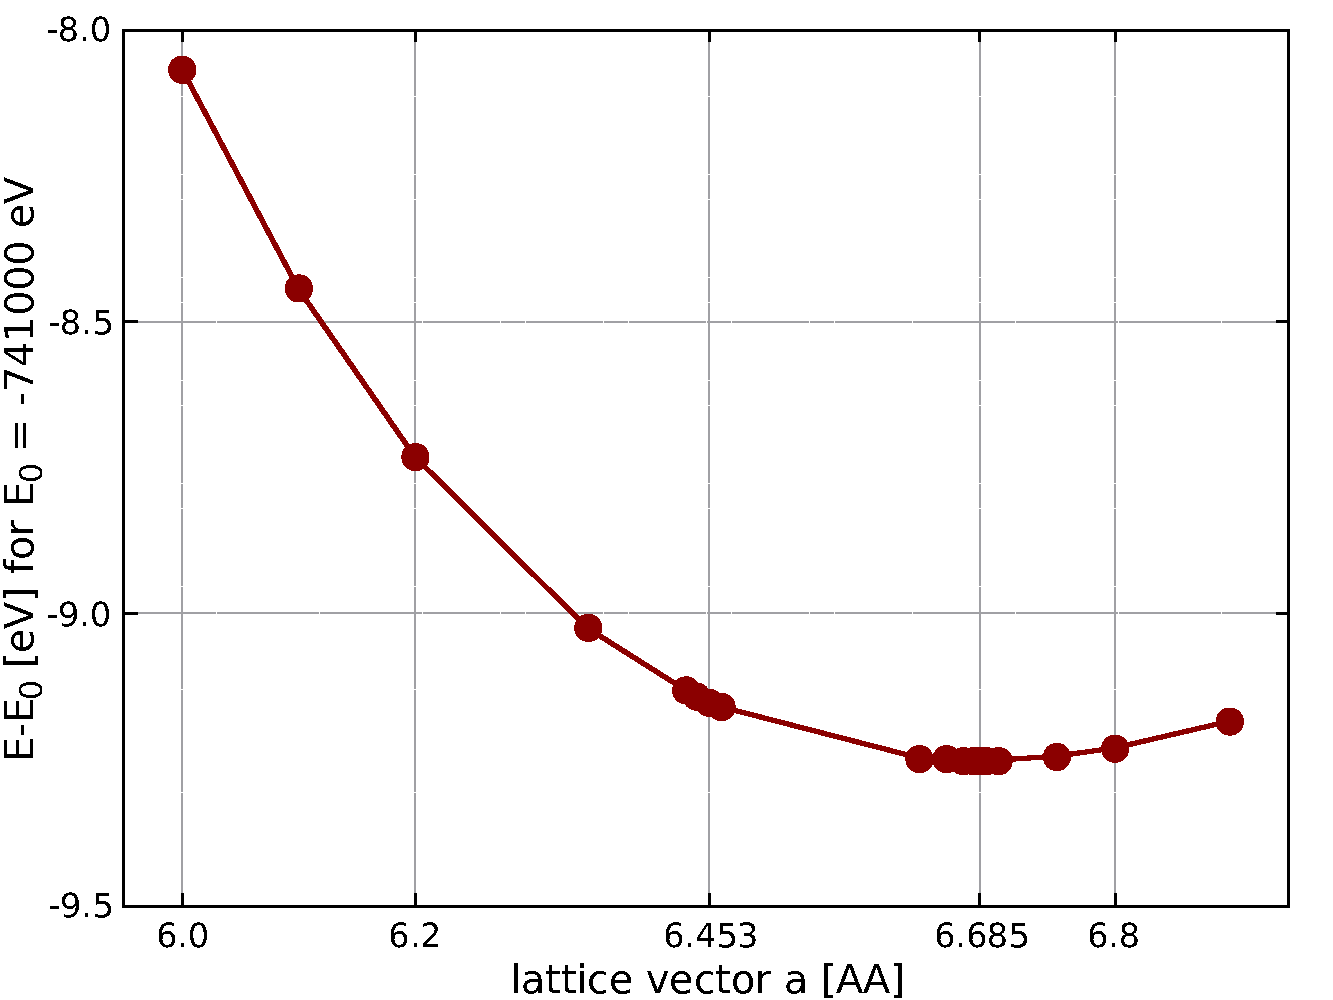
\includegraphics[width=\linewidth]{andere_bilder/lattice_constant_study_spin_none_no_soc.pdf}
		\caption{Lattice constant $a$ with respect to the total energy. The lowest energy was found for 6.685 Angström.}\label{lattice_constant}  \vspace{12.5pt}
	\end{minipage}
\end{figure}

	First of all the lattice constant $a$ with the lowest total energy in the HgTe bulk must be determined, since the energetically most stable constitution of a crystal structure is given by the smallest total system energy respective to the lattice constant.  
%because this one will be the most stable lattice constant.
	Both the bulk and the slab calculations must have the right values for the k-grid density in order to make calculations faster and less computationally expensive. 		
%At the same time, the bulk calculations, and also the ones for the surface, are in need of the right choice of the k-grid parameters. 

	In figure \ref{kgrid_lattice_constant} one can see the result for lattice vector $a$ in Angström with respect to the total energy of the bulk, with different k-grids. It is clear, that 3x3x3 gives no representative results. 
%Here the lattice constant also doesn't have a minimum. 

	After carefully looking at the results of the energy convergence tests, the lattice constant was determined by using a higher k-grid than 8x8x8 to be sure about the convergence of the calculations. The result of the final step to determine the best theoretical value of the lattice constant for our crystal structure can be seen in figure \ref{lattice_constant}.
%	and the one with the lowest energy was 6.685 Angström. 
	As one can see, the best results were obtained for a lattice constant of 6.685 Angström.

%	Then the k-grid study was done again just for this lattice constant. In figure \ref{k_grid_study} there is the outcome of the bulk k-grid and additionally the ones for 4 layers, 8 layers and 16 layers. And now it makes sense that in figure \ref{kgrid_lattice_constant} that above 8 the graphs are identical. The energy doesn't change for higher k-grids. 
	It is this lattice constant, that was used for executing a detailed k-grid study. The results of this study is shown in figure \ref{k_grid_study} where additionally the results for the slabs with 4, 8 and 16 layers are illustrated.  
	It is not surprising that the most economic values of the k-grids for the slabs are virtually the same as for the bulk namely around 12x12x12. But since for higher k-grids the band structure curve becomes smoother, we used 24x24x24 in order to get smooth results. 
	Note that although the CPU time therefore increases, this is not significant for the calculations of the systems regarded in this thesis. 
%	For the slabs the graphs look a bit different. The convergence is not as smooth as for the bulk and the k-grid must be higher for a physical output. 
%	Theoretically, the higher the k-grid, the smoother the band structure or dos output. But the CPU time is also increasing. This means, one has to choose a k-grid some where in the middle. I used 24 points per direction for all following calculations. 
\begin{figure}[b!]
	\begin{subfigure}[c]{.5\linewidth}
		\centering
		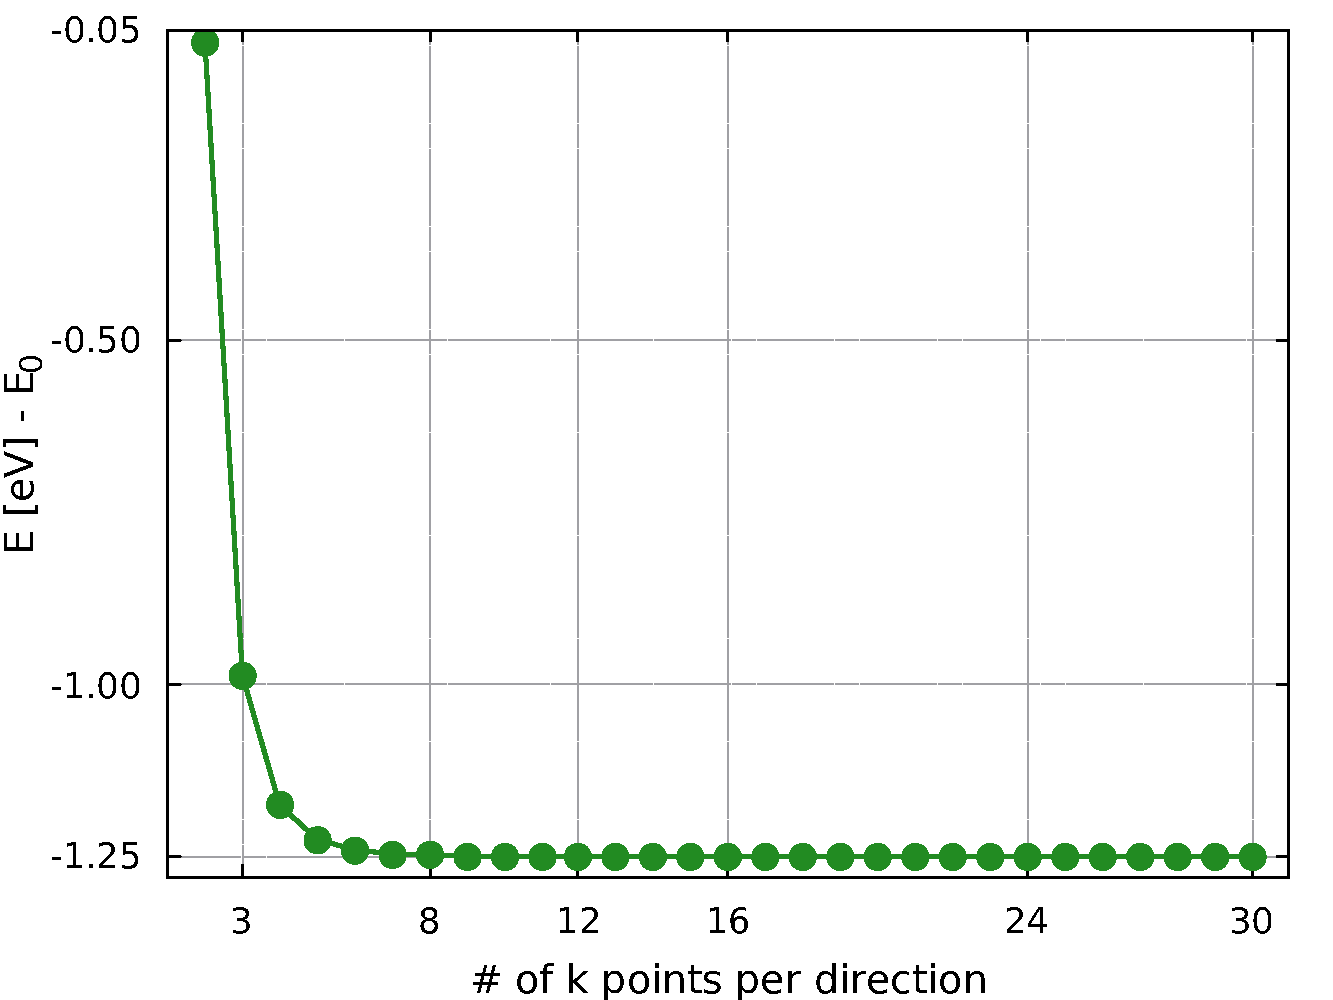
\includegraphics[width=\linewidth]{andere_bilder/kgrid_bulk.pdf}
		\caption{Bulk with $E_0= -741008 \,\unit{eV}$} \label{k_grid_1}
		\vspace{5pt}
	\end{subfigure}
	\hfill
	\begin{subfigure}[c]{.5\linewidth}
		\centering
		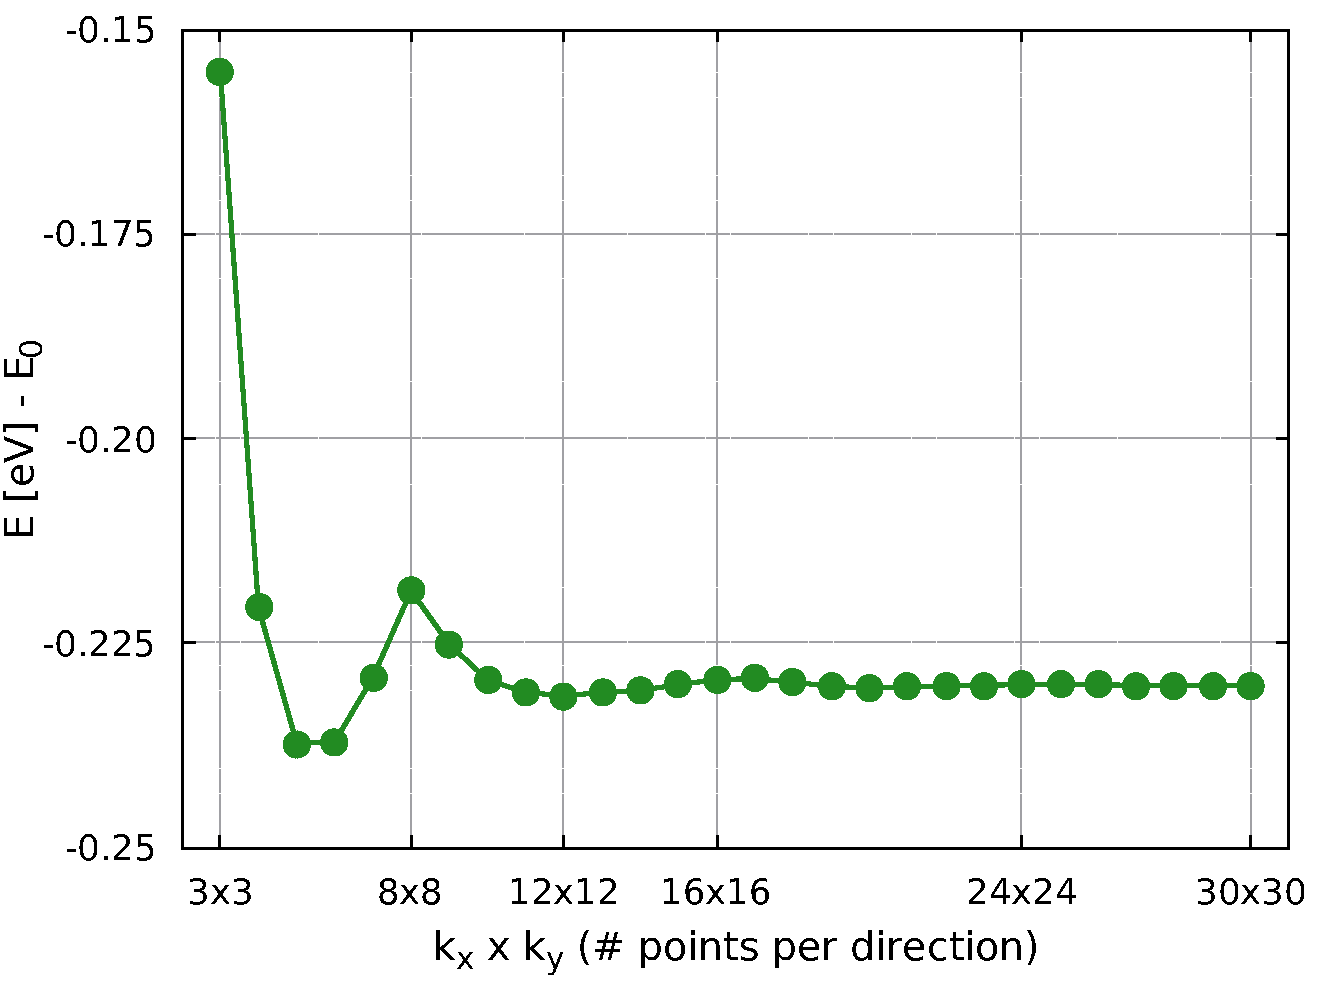
\includegraphics[width=\linewidth]{andere_bilder/kgrid_1x1x4_layers.pdf}
		\caption{Slab with 4 layers with $E_0= -1482047 \,\unit{eV}$} \label{k_grid_2}
		\vspace{5pt}
	\end{subfigure}
	\begin{subfigure}[c]{.5\linewidth}
		\centering
		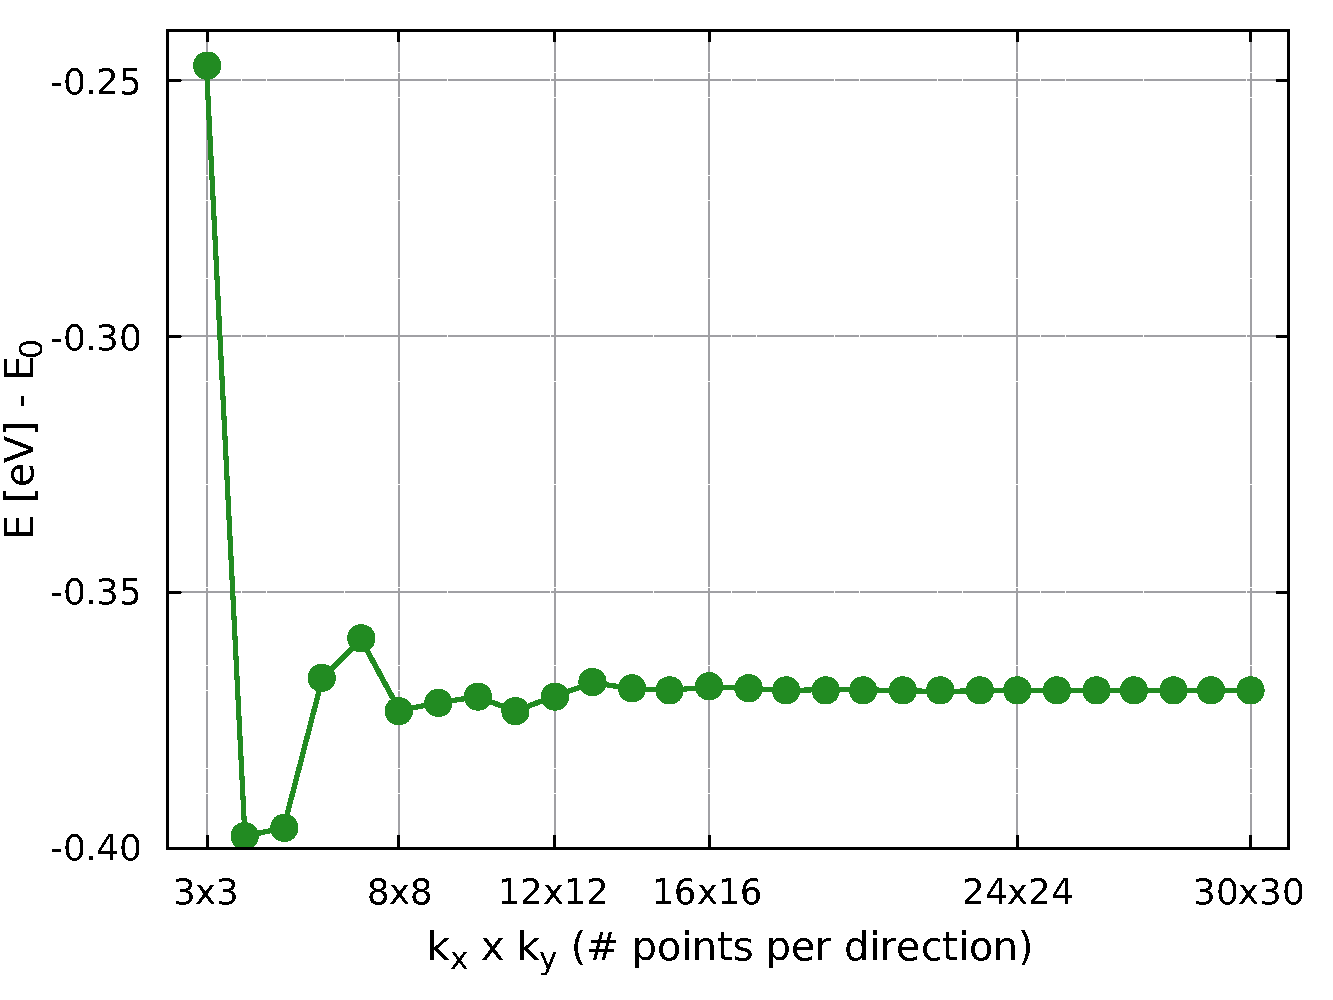
\includegraphics[width=\linewidth]{andere_bilder/kgrid_1x1x8_layers.pdf}
		\caption{Slab with 8 layers with $E_0= -2964065 \,\unit{eV}$} \label{k_grid_3}
	\end{subfigure}
	\hfill
	\begin{subfigure}[c]{.5\linewidth}
		\centering
		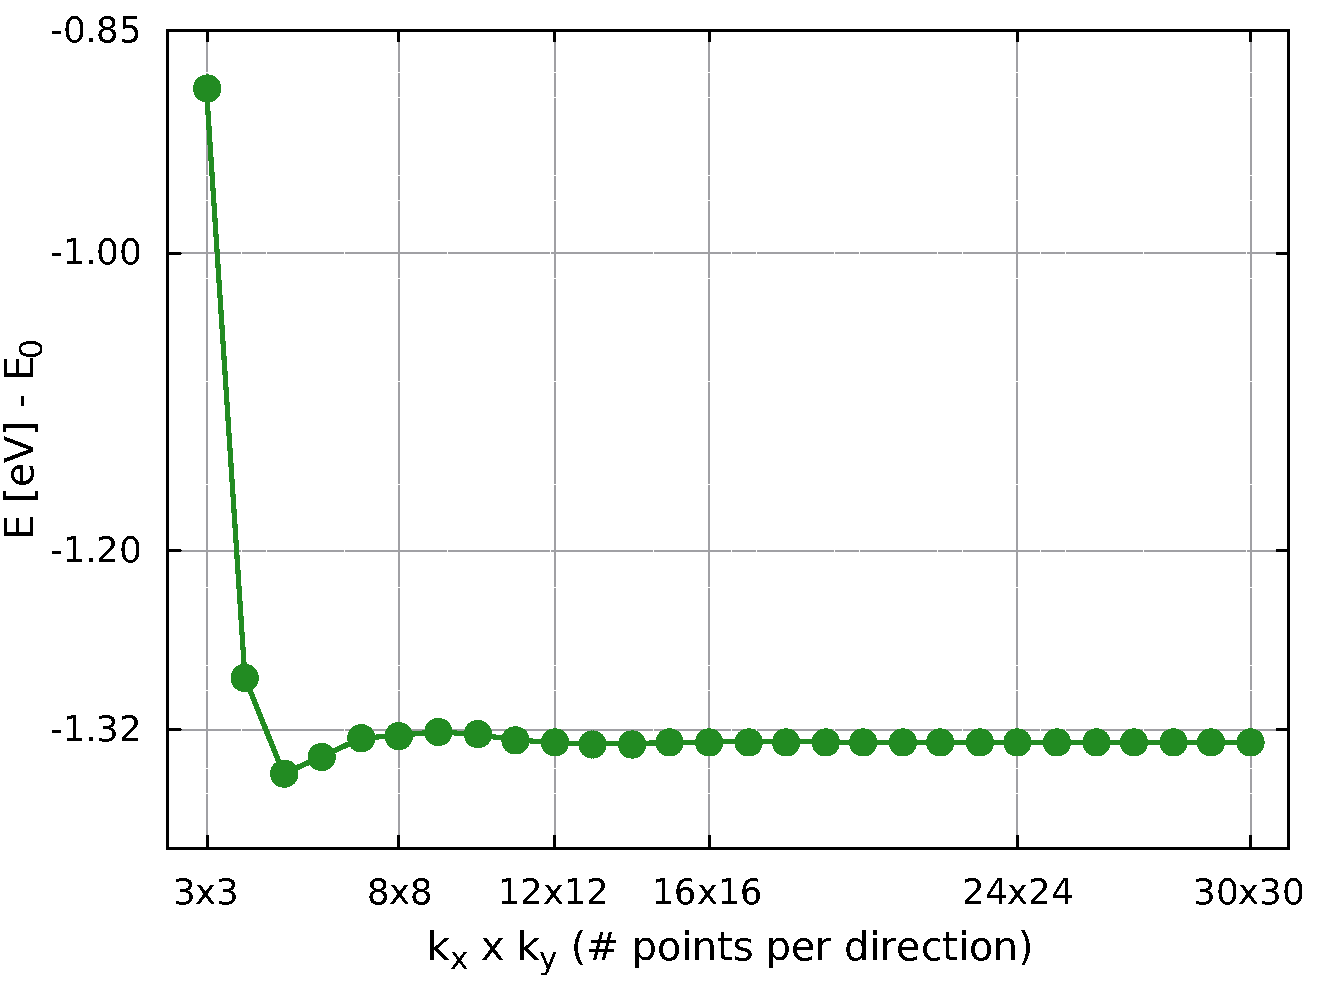
\includegraphics[width=\linewidth]{andere_bilder/kgrid_1x1x16_layers.pdf}
		\caption{Slab with 16 layers with $E_0= -5928101 \,\unit{eV}$} \label{k_grid_4}
	\end{subfigure}
	\caption{Total energy $E [\unit{eV}] - E_0$ (with $E_0$ the energy offset) as a function of k-grid spacing.} \label{k_grid_study}
\end{figure}

\FloatBarrier	
	%%% Local Variables:
	%%% mode: latex
	%%% TeX-master: "main_BA2.0"
	%%% End:
	
	\subsection{The bulk band structure in the first 3D Brillouin zone}
		The calculations for the bulk band structure are made in the 3D Brillouin zone.
%	The ways of integration in $\kk$-space can be chosen different, but it must be connected. 
	For the calculation of the bulk band structure, we use the following path (like in \cite{tutorial2} p.12)
	\begin{align}
		\text{L} \rightarrow \Gamma \rightarrow \text{X} \rightarrow \text{W} \rightarrow \text{K}
	\end{align} 
	Those symmetry points are illustrated in figure \ref{brillouin_zone} in the theory part. The k-grid and 
%	command for the band structure output is defined in the control.in as
	the command used in order to extract the band structure output from FHI-aims is defined in the control.in file as
	\\
	\begin{minipage}[c]{\linewidth}	\vspace{15pt}
		\begin{verbatim}
		# k_grid settings
		k_grid	24	24	24
		#
		# output band structure
		output band 0.5   0.5   0.5    0.0   0.0   0.0    21  L     Gamma
		output band 0.0   0.0   0.0    0.0   0.5   0.5    21  Gamma X
		output band 0.0   0.5   0.5    0.25  0.5   0.75   21  X     W
		output band 0.25  0.5   0.75   0.375 0.375 0.75   21  W     K
		\end{verbatim} \vspace{0.2cm}
	\end{minipage}
%	The number 21 is the number of $\kk$ points that are computed between two high symmetry points.
	The geometry.in input is the same as the one mentioned in subsection \ref{FHI-aims}. 	
	\begin{figure}[b!]
		\centering
		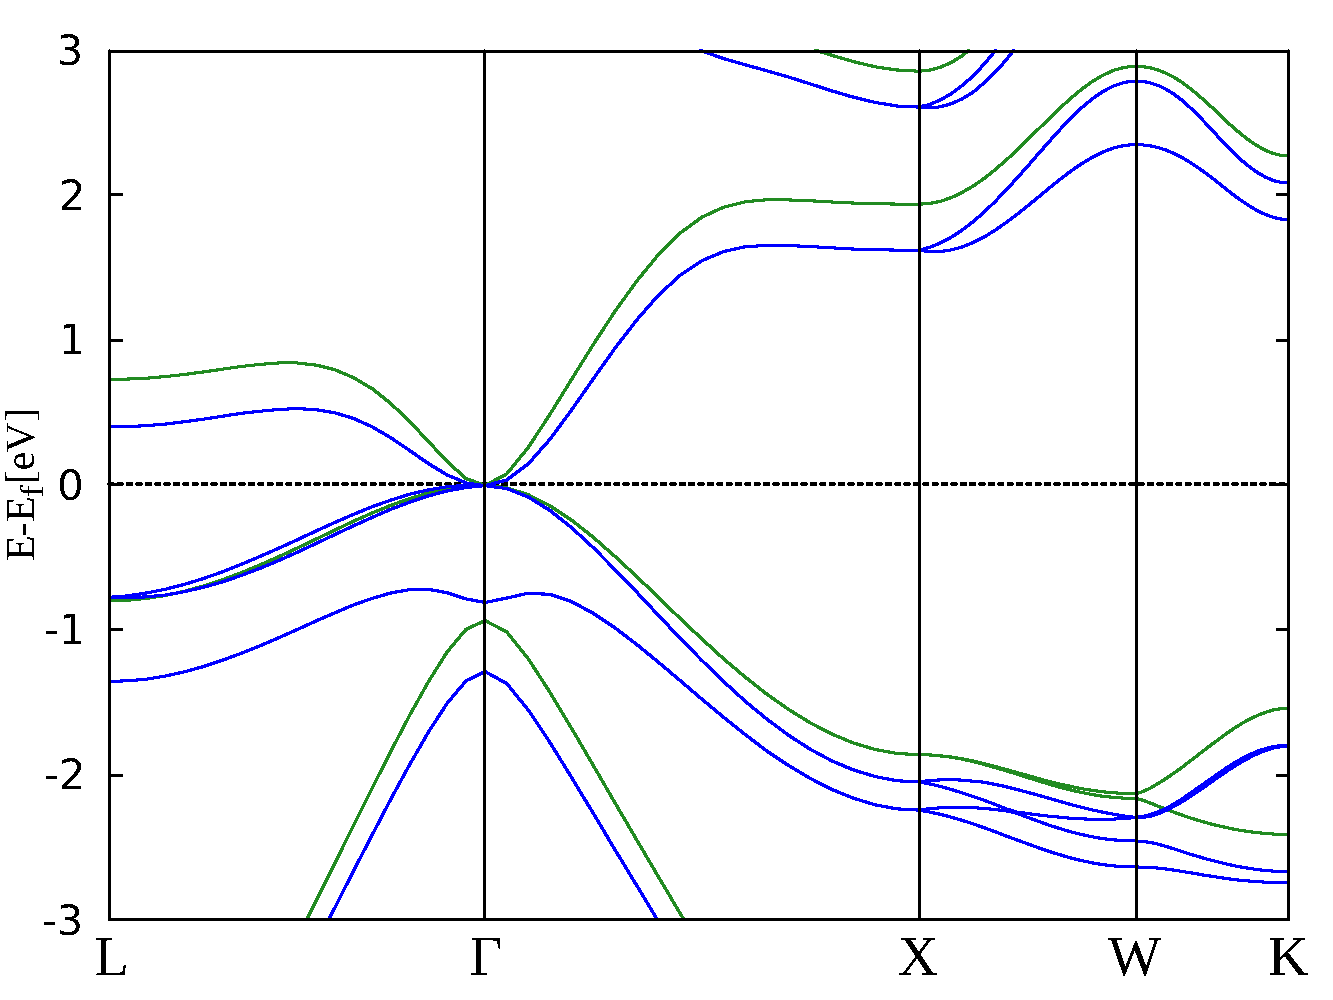
\includegraphics[width=.7\linewidth]{andere_bilder/plot_bulk_with_without_soc.pdf}
		\caption{Band structure of bulk HgTe in the first 3D Brillouin zone. The green lines are the band structure without spin-orbit coupling, and the blue ones include spin-orbit coupling. The Fermi level is indicated by the dashed line.} \label{bulk_band_structure}
	\end{figure}
	
	The outcome of the band structure calculations is shown in figure \ref{bulk_band_structure}, where the green lines indicate the band structure without spin-orbit coupling (SOC) and the blue lines are the calculations with SOC. 
%	Note that the two different band structures just overlap near and at the $\Gamma$ point. 
%%% Local Variables:
%%% mode: latex
%%% TeX-master: "main_BA2.0"
%%% End:
	
	\subsection{Projected bulk band structure}
		As mentioned before, the band structure of the bulk is calculated along the high symmetry points in the 3D Brillouin zone, see figure \ref{brillouin_zone}.  
%	But for comparing this band structure with the slabs band structure, the bulk must be represented in a different way, which is called projected bulk band structure (PBBS).
	But to compare the bulk band structure with the surface band structure from the slab, the bulk must be analyzed by using the so-called projected bulk band structure (PBBS).
	By superimposing the plots of the slab’s band structure with the PBBS, the bulk states can be distinguished from the surface states.  
	
%	The \kk-grid had $k_x$, $k_y$ and $k_z$ for the repetition in all directions.
	The periodic boundary conditions are applied in all directions when we get the band structure for the bulk. As we mentioned in subsection \ref{surface_modeling}, this is not applicable when we perform the calculations for the surface band structure in the supercell approach for an isolated slab.
%	But the slab doesn't have the same boundary condition in the $k_z$ direction.
	The slab band structure cannot be calculated like the bulk band structure, because for the surface the translation symmetry is broken. Thus we have to find an other solution how to compare the information about those two systems. At first it must be ensured that the orientation is the same, then we perform band structure calculations for different $k_z$ values of the bulk. In other words, we make 2D slices of the first 3D Brillouin zones of the bulk such that $k_z$ is perpendicular to them.
	Once these calculations are done, we put them all together in an ensemble which then represents the PBBS in that direction.
	As soon as we have the PBBS, we can compare it with the band structure of the slabs in the (001) growing plane. 
	For this purpose, we calculate the band structure by following the path through the high symmetry points in the 2D Brillouin zone:	
%	Instead of the whole crystal, there is just one cleavage of the bulk regarded, in our case the (001) plane. In other words the 3D Brillouin zone cannot represent the surface band structures, thus the number $k_z$ is wrong for the slab calculations, but with many slices of the 2D Brillouin zone one can reconstruct the bulk band structure and the surface band structure in one plot.
%	
%	The high symmetry points of the 2D Brillouin zone of the (001) cleavage were already shown in \eqref{2D-BZ-points} and the integrating way I chose is
	\begin{align}
		\overline{\text{J}} \rightarrow \overline{\Gamma} \rightarrow \overline{\text{K}} \rightarrow \overline{\text{J}}
	\end{align}
	The band structure for the slabs will look different for different terminations of the surface while we follow the same path along the high symmetry points.
	The lines which lie in the gap are energy bands corresponding to surface states, which can be trivial surface states or topological surfaces states. 
%	to see the band structure of all connections and the Gamma in the middle because thats the most interesting symmetry point for HgTe. 
%	Unfortunately, FHI-aims always applies periodic boundary conditions, but there is still a possibility to omit that problem. 
	In practical terms, we proceed by exchanging the $k_z$ in output instructions in the control.in file by different values. 
%	First of all, the \kk-grid is now $k_x$, $k_y$ and 1. In the band structure output part of the control.in, the high symmetry points must be inserted like in \eqref{2D-BZ-points} but the last component, the $k_z$, must be adjusted for the bulk calculations.
	In sufficient small steps $k_z$ goes from $k_z=0$ to $k_z=k_{z,\text{max}}$, with $k_{z,\text{max}} = \frac{\pi}{a}$ where $a$ is the lattice constant. This value of the kz corresponds to the edge of the first BZ.
%	which is half of the $z$-component of the reciprocal vector $b_3$ in \eqref{fcc_reciprocal_vectors}, which is the edge of the first Brillouin zone. It emerged that 40 slices are enough to get a nice plot. 
	
%	For the calculations with the supercells, $k_z$ must be set to 0 because otherwise the boundary condition in that direction is wrong considered by FHI-aims.
	Regarding the calculations of the band structure for the slab, we need to take into account that since we have a 2D Brillouin zone, the path along the Brillouin zone through the high symmetry points must be in the same plane. In our case, since we are interested in the (001) direction, we need to set $k_z = 0$ in order to get the energy bands.
	
%	The k-grid is the same as in the bulk band structure in 3D BZ. The band structure command written in the control.in for the bulk slice $k_z=1/40\cdot k_{z,\text{max}}$ is 
	Here is an example of how to plot one slice of the Brillouin zone in the PBBS, where the slice is at $k_z = 1 / 40 * k_{z,max}$:
	\\
	\begin{minipage}[c]{\linewidth}	\vspace{15pt}
		\begin{verbatim}
			# output band structure
			output band 0.5   0.0   0.01175   0.0   0.0   0.01175    80  J     Gamma
			output band 0.0   0.0   0.01175   0.5   0.5   0.01175    80  Gamma K
			output band 0.5   0.5   0.01175   0.5   0.0   0.01175    80  K     J
		\end{verbatim} \vspace{0.2cm}
	\end{minipage}
	
	The three numbers after the term \texttt{output band} are indicating the point in the path where one starts the calculation for the energy band in the reciprocal space, while the fourth to the sixth number are the coordinates for the point of the path where one finishes the energy band calculation in the reciprocal space.
	The last number: \texttt{80} is the number of points which divides that segment of the path. The sharpness of the energy bands depends on the k-grid density and the number of points you take in each segment.	
	The letters at the end of the line are labeling the first point and the final point of the calculation through the path.
%	Note that the labeling at the end is just for identifying the points in the output and aims does not recognize special signs, hence it is neither possible nor necessary to add a bar or other notations.  
	
	As final comment, remark that we choose 80 as parameter to compute the energy bands along a segment after 21 points for the calculations of figure \ref{bulk_band_structure} led to bands that where not smooth at some point.
%	The number 80 is the number of $\kk$ points that are computed between two high symmetry points. The reason for the higher number of points is, that, as seen in figure \ref{bulk_band_structure} the plot is not very smooth with a small number, so here a higher number was chosen. 

	As we explained at the beginning of this subsection, once the band structures are calculated for several values of $k_z$, we then have to put all bands in a single plot in order to visualize the PBBS. This situation can be seen in figure \ref{bulk_band_structure_generation}.
%	The output of all slices finally needs to be plotted in one single plot. In figure \ref{bulk_band_structure_generation} a few intermediate steps are illustrated plus the final projected bulk band structure part \ref{bulk_PBBS}. 

	In the figures \ref{bulk+surface_even_layers}, \ref{bulk+surface_odd_layers_Te} and \ref{bulk+surface_odd_layers_Hg} we represent the plots of the band structures for Te-Hg termination for 4, 8 and 16 layers. 
%	and each Hg and Te termination separately in 5, 9 and 17 layers, every termination with and without hydrogen. 
	In these figures, we can also see the band structure calculation for slabs which have symmetric Te-Te and Hg-Hg terminations, as well as the band energies corresponding to the different terminations with or without passivation by hydrogens at one surface.
	
	The grey part is the PBBS part, the blue lines are the band structure of the slabs and the red line marks the Fermi level.  	
	\begin{figure}[htbp]
		\begin{subfigure}[c]{.48\linewidth}
			\centering
			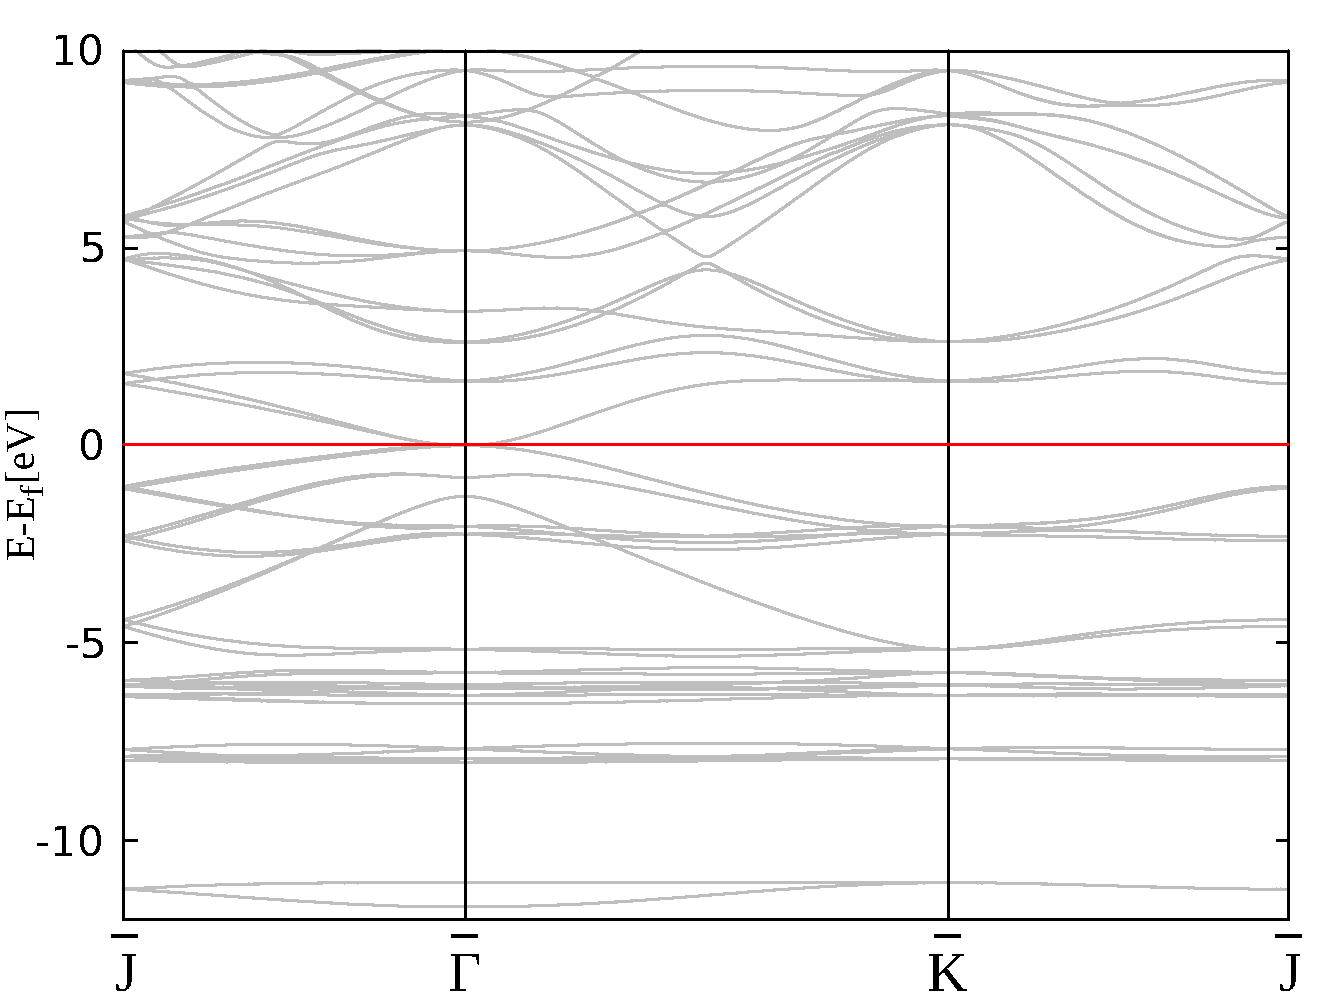
\includegraphics[width=\linewidth]{andere_bilder/0_bulk_-12_10.pdf}
			\caption{PBBS for $k_z$ is equal to zero.}
			\vspace{14pt}
		\end{subfigure}
		\hfill
%		\begin{subfigure}[c]{.48\linewidth}
%			\centering
%			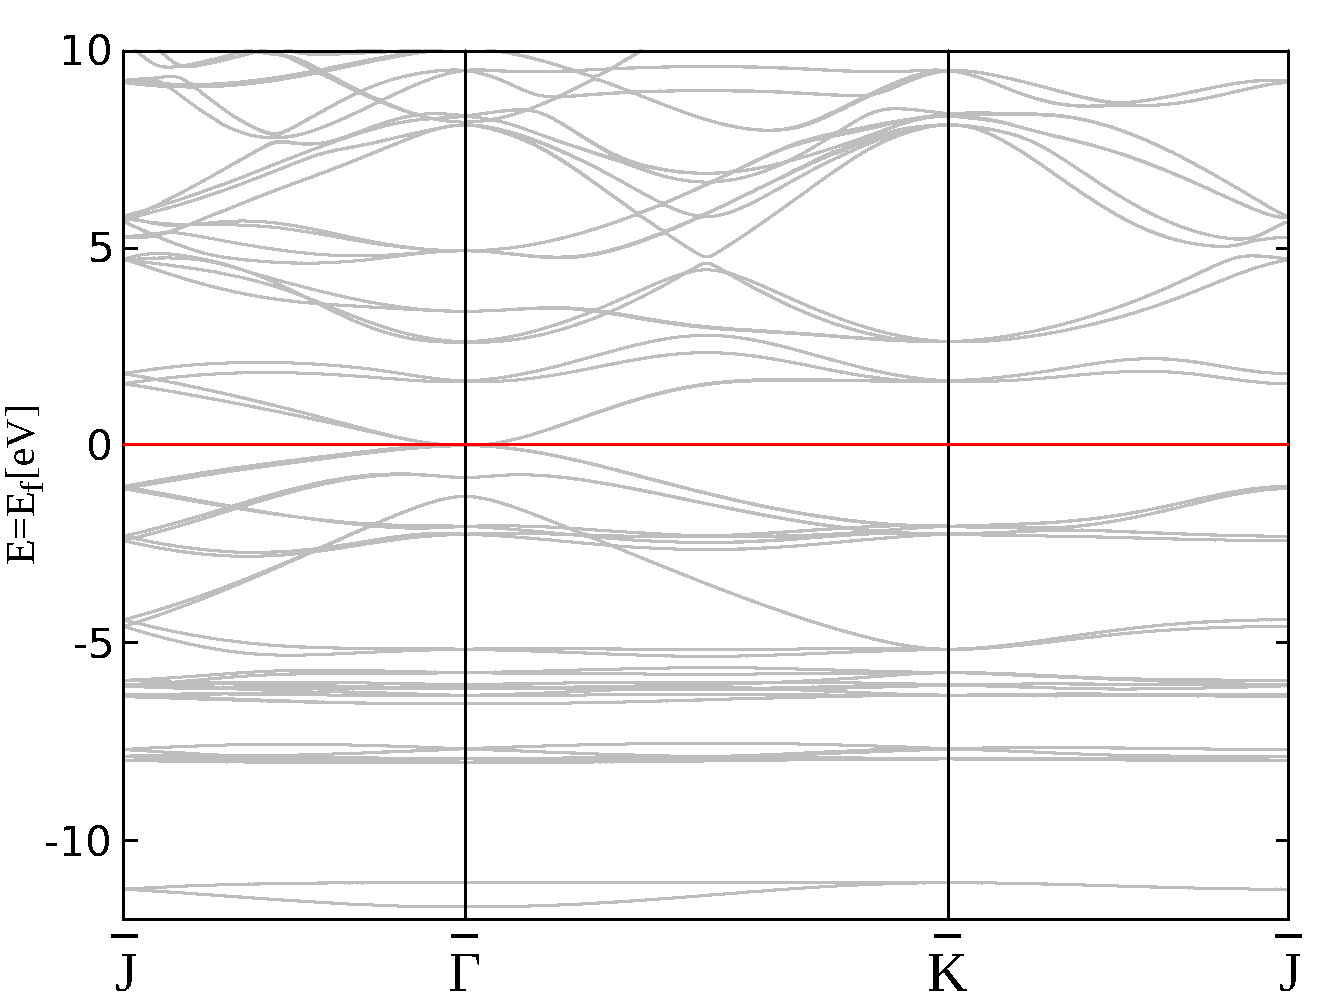
\includegraphics[width=\linewidth]{2_bulk_-12_10.pdf}
%			\caption{PBBS calculations with $k_z = 0$, $1/40\cdot k_{z,\text{max}}$, $1/20\cdot k_{z,\text{max}}$}
%		\end{subfigure}
		\begin{subfigure}[c]{.48\linewidth}
			\centering
			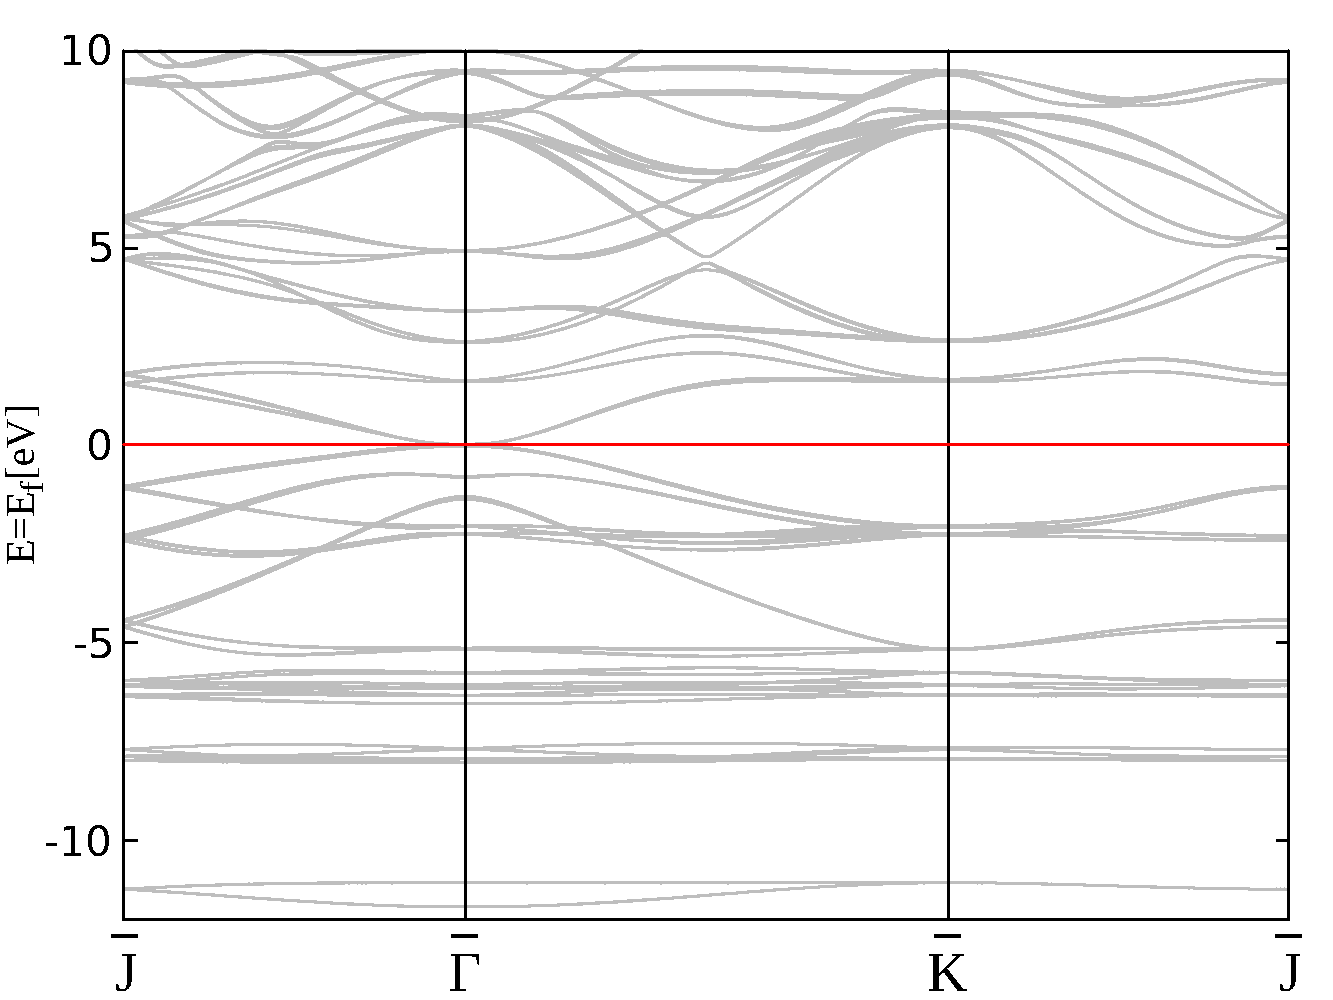
\includegraphics[width=\linewidth]{andere_bilder/4_bulk_-12_10.pdf}
			\caption{Ensemble for PBBS for $k_z$ having values from 0 to $1/10\cdot k_{z,\text{max}}$}
		\end{subfigure}
%		\hfill
%		\begin{subfigure}[c]{.48\linewidth}
%			\centering
%			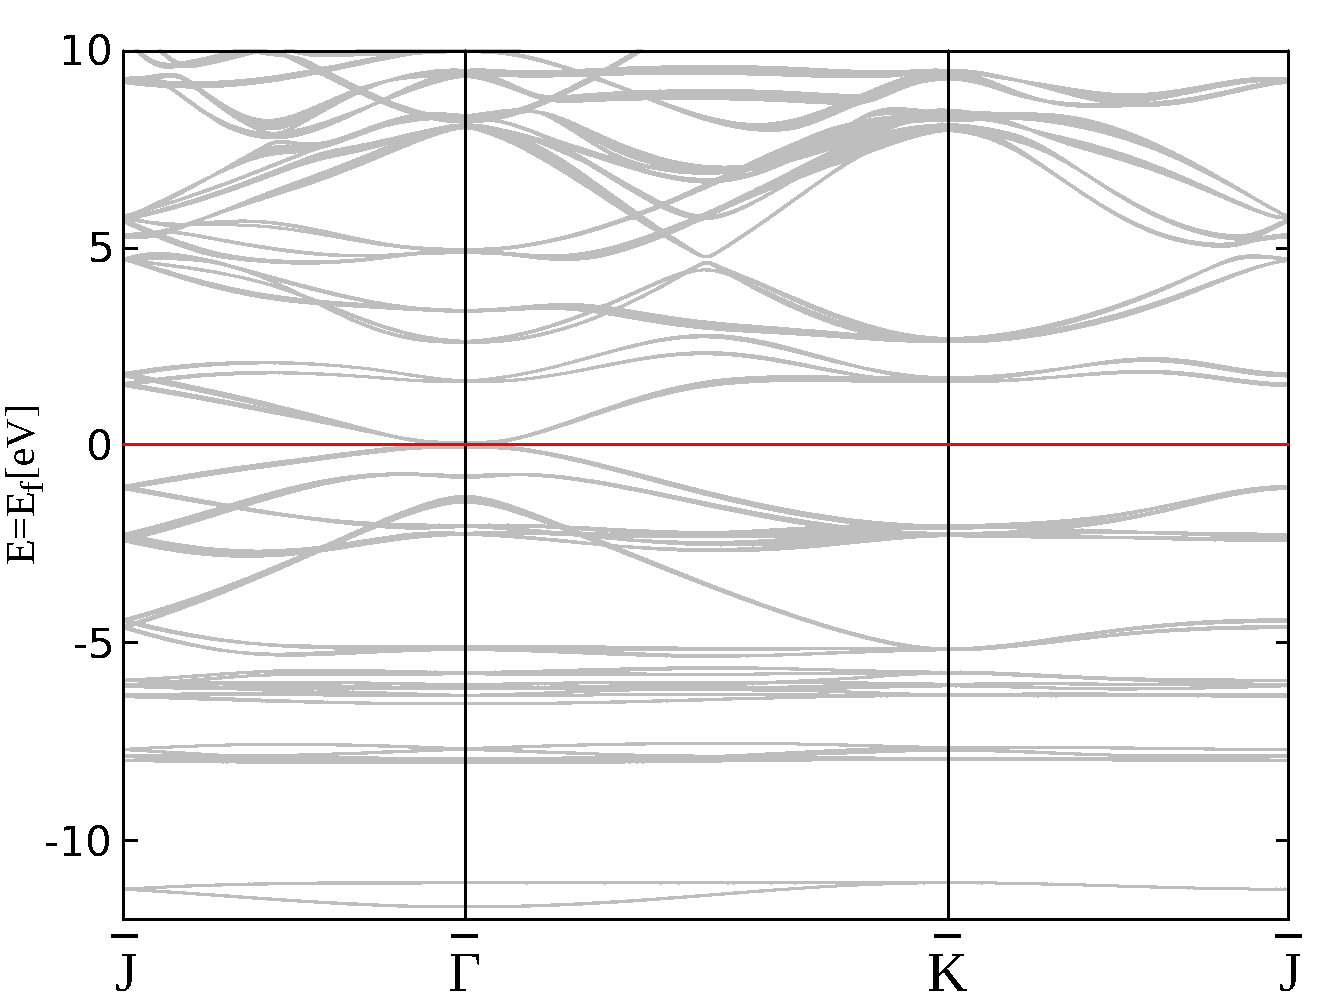
\includegraphics[width=\linewidth]{6_bulk_-12_10.pdf}
%			\caption{PBBS calculations with $k_z$ from 0 to $6/40\cdot k_{z,\text{max}}$}
%		\end{subfigure}
		\begin{subfigure}[c]{.48\linewidth}
			\centering
			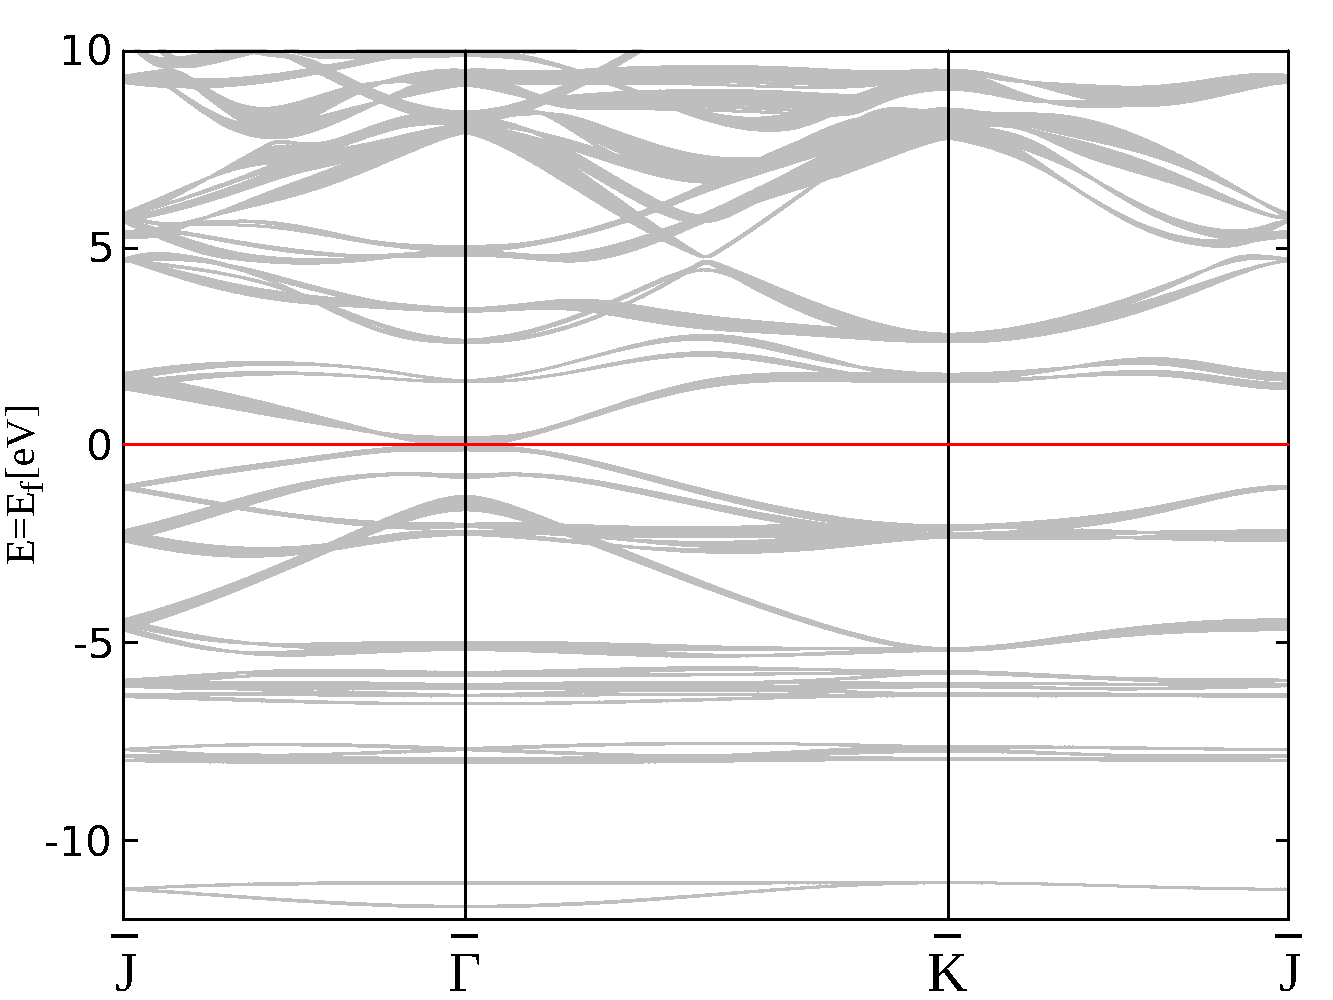
\includegraphics[width=\linewidth]{andere_bilder/10_bulk_-12_10.pdf}
			\caption{Ensemble for PBBS for $k_z$ having values from 0 to $1/4\cdot k_{z,\text{max}}$} 
		\end{subfigure}
		\hfill
		\begin{subfigure}[c]{.48\linewidth}
			\centering 
			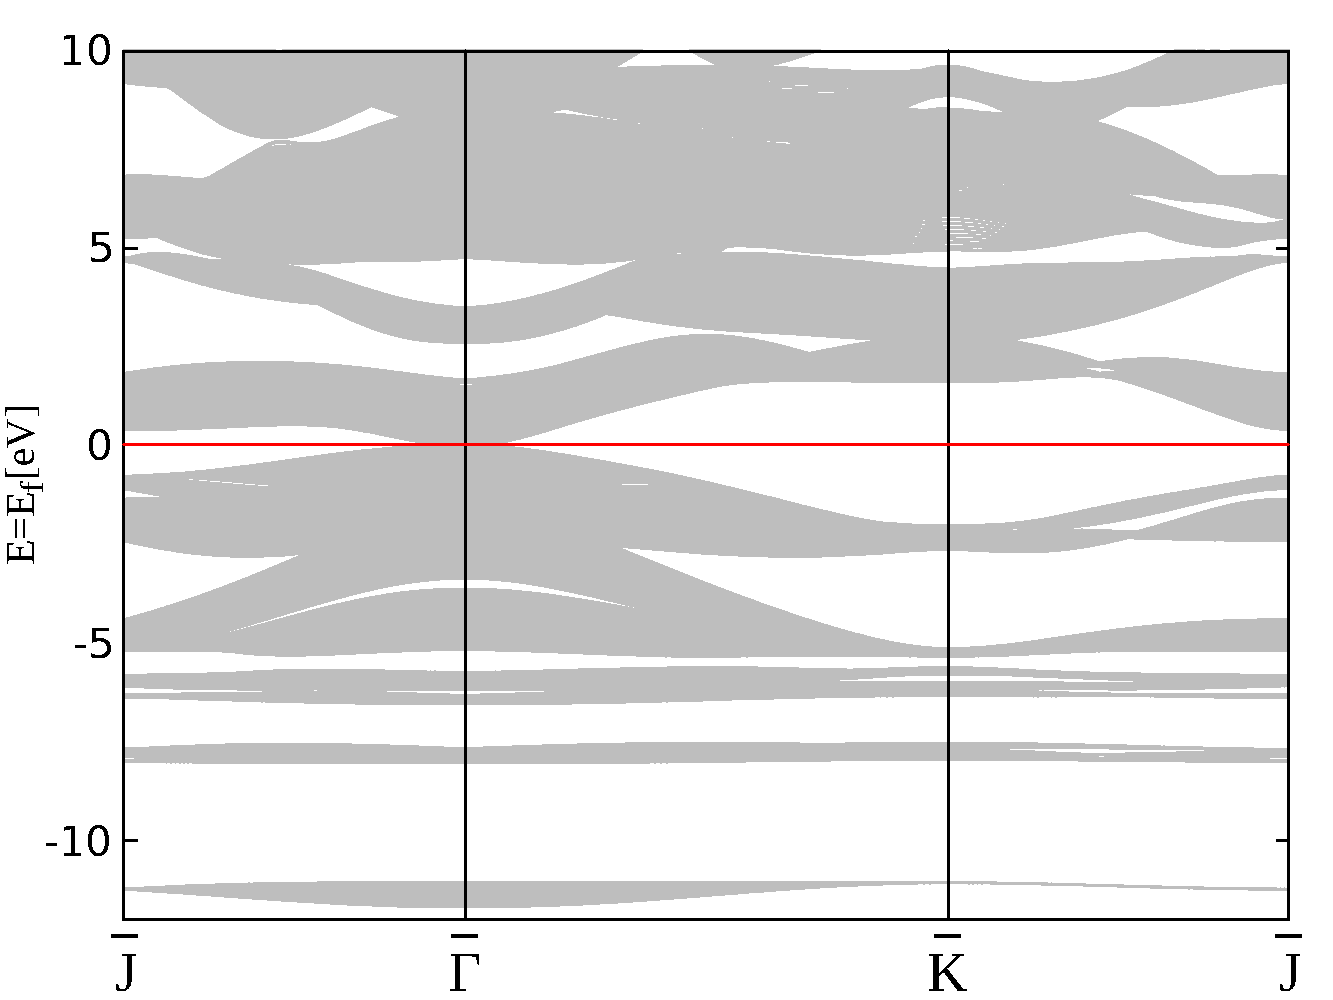
\includegraphics[width=\linewidth]{andere_bilder/bulk_-12_10.pdf}
			\caption{Whole PBBS for all the values of $k_z$ going from 0 to $k_{z,\text{max}}$} \label{bulk_PBBS}
		\end{subfigure}
		\caption{Generation of projected bulk band structure of HgTe} \label{bulk_band_structure_generation}
	\end{figure}

%Te-Hg termination	
	\begin{figure}[htbp]
		\begin{subfigure}[c]{.48\linewidth}
			\centering
			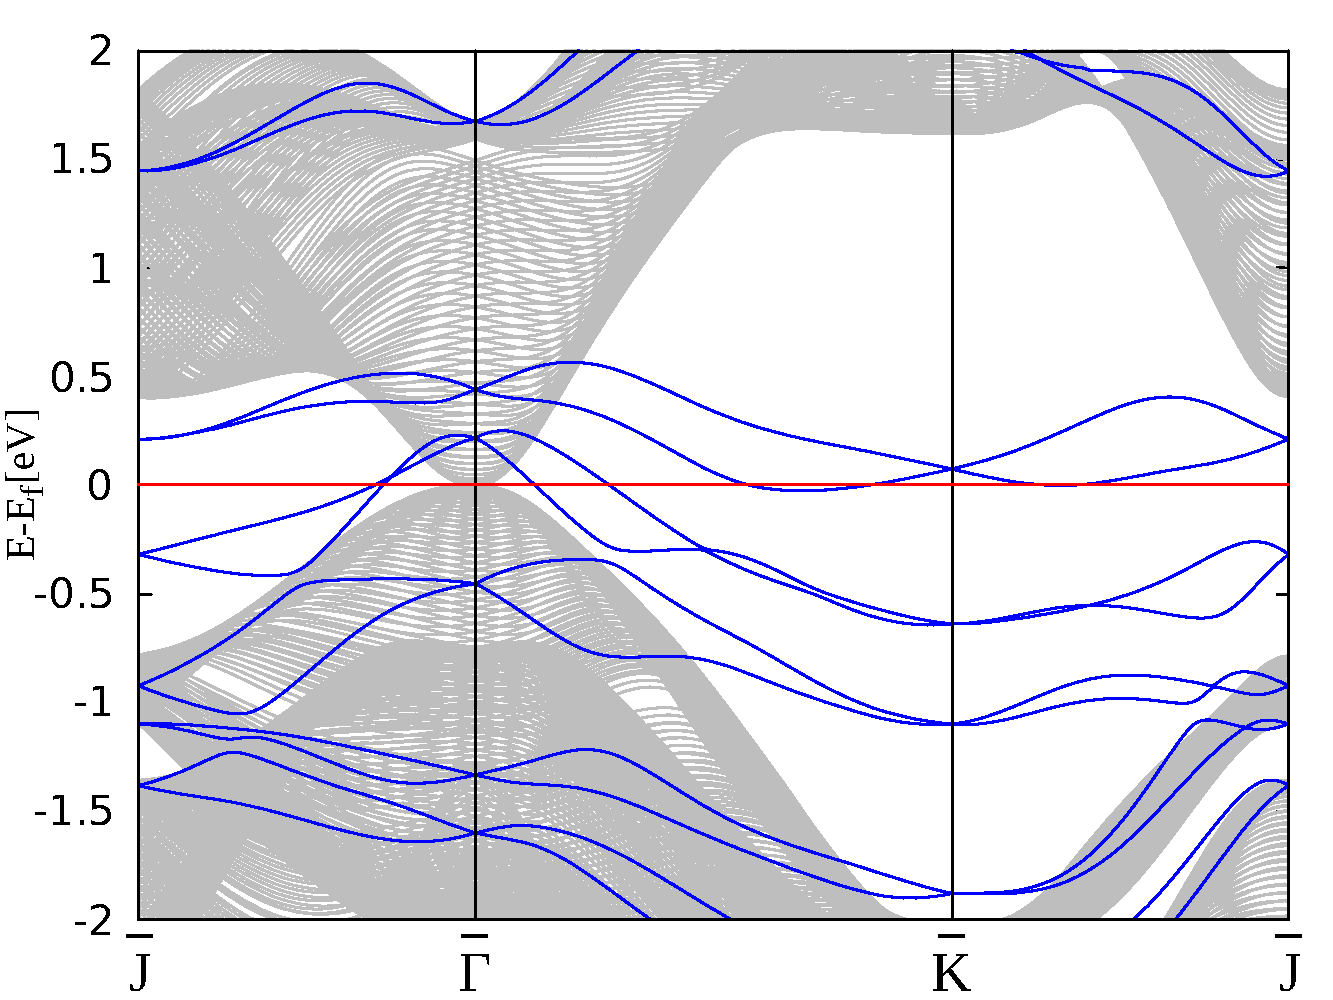
\includegraphics[width=\linewidth]{Te_and_Hg_termination/no_H_bulk+4_layers_no_dos_-2_2.pdf}
			\caption{4 layers without hydrogens passivating the Te termination}
		\end{subfigure}
		\hfill
		\begin{subfigure}[c]{.48\linewidth}
			\centering
			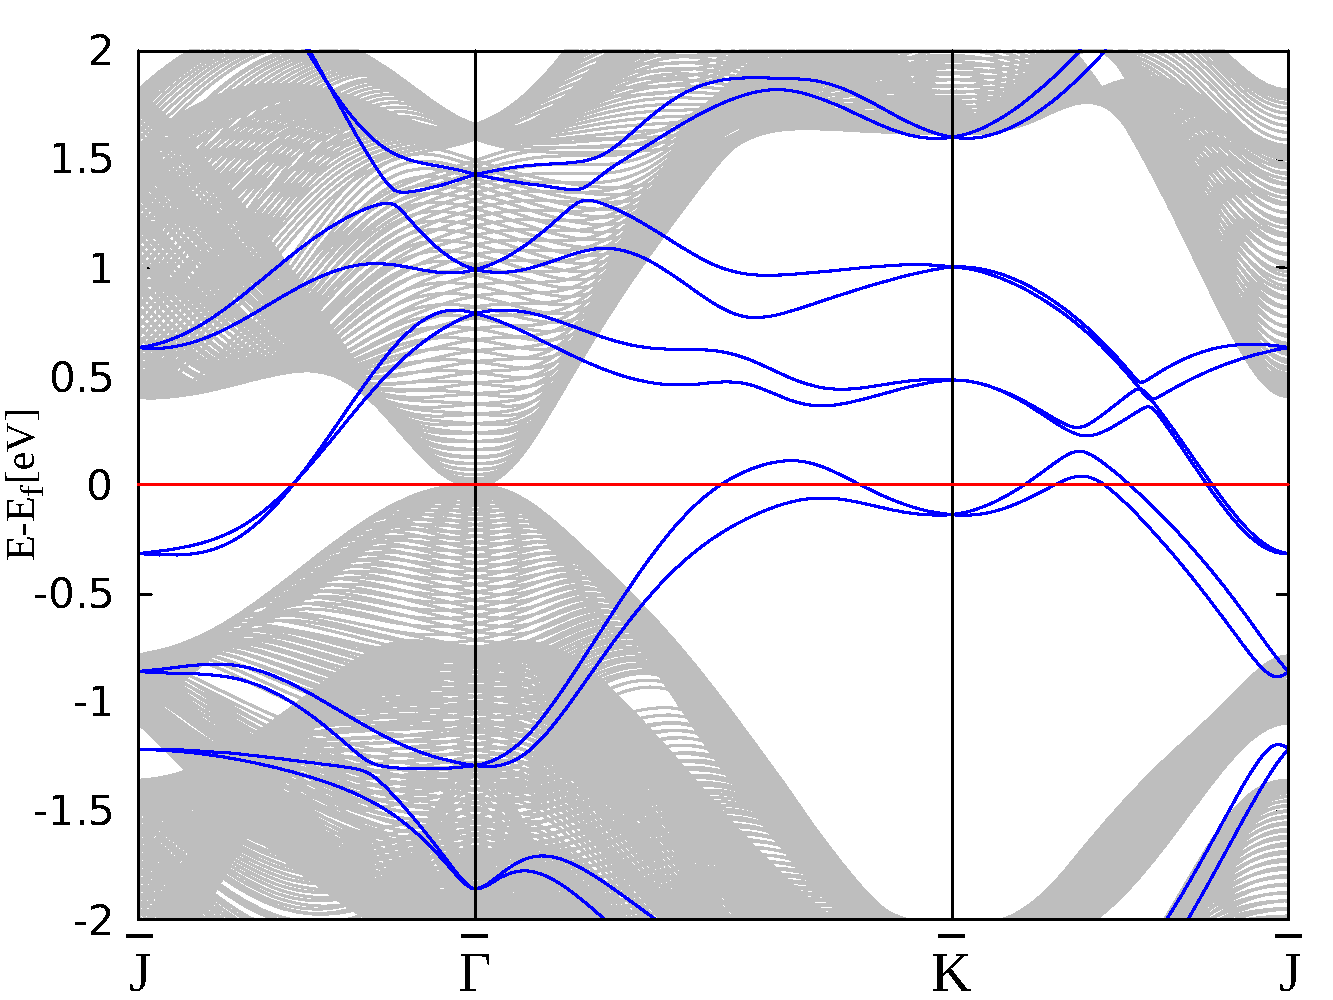
\includegraphics[width=\linewidth]{Te_and_Hg_termination/bulk+4_layers_no_dos_-2_2.pdf}
			\caption{4 layers with hydrogens on the bottom passivating the Te surface terminations}
		\end{subfigure}
		\begin{subfigure}[c]{.48\linewidth}
			\centering
			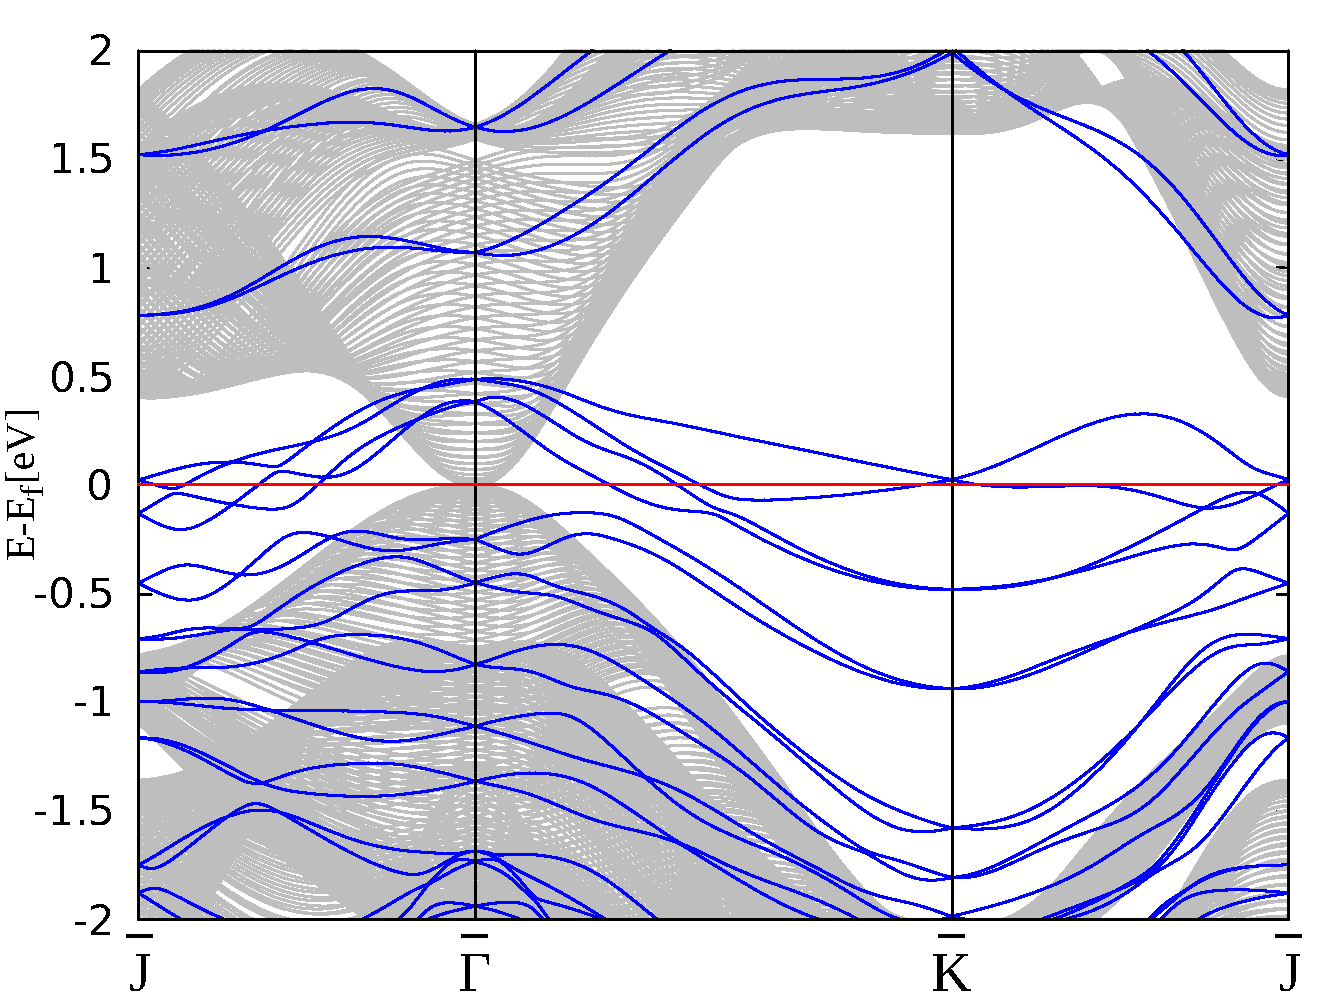
\includegraphics[width=\linewidth]{Te_and_Hg_termination/no_H_bulk+8_layers_no_dos_-2_2.pdf}
			\caption{8 layers without hydrogens passivating the Te termination}
		\end{subfigure}
		\hfill
		\begin{subfigure}[c]{.48\linewidth}
			\centering
			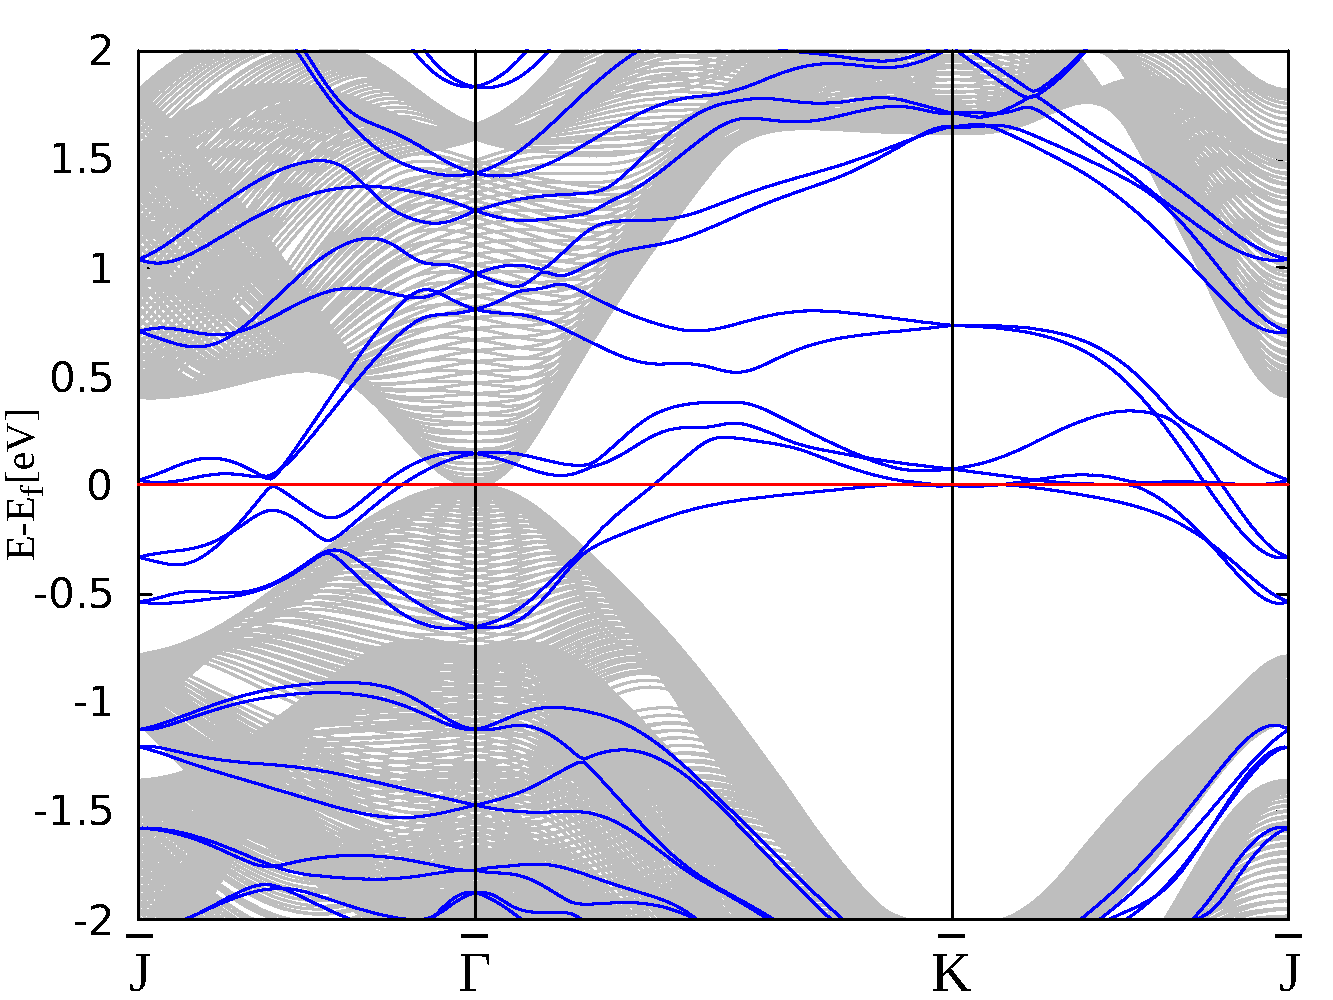
\includegraphics[width=\linewidth]{Te_and_Hg_termination/bulk+8_layers_no_dos_-2_2.pdf}
			\caption{8 layers with hydrogens on the bottom passivating the Te surface terminations}
		\end{subfigure}
		\begin{subfigure}[c]{.48\linewidth}
			\centering 
			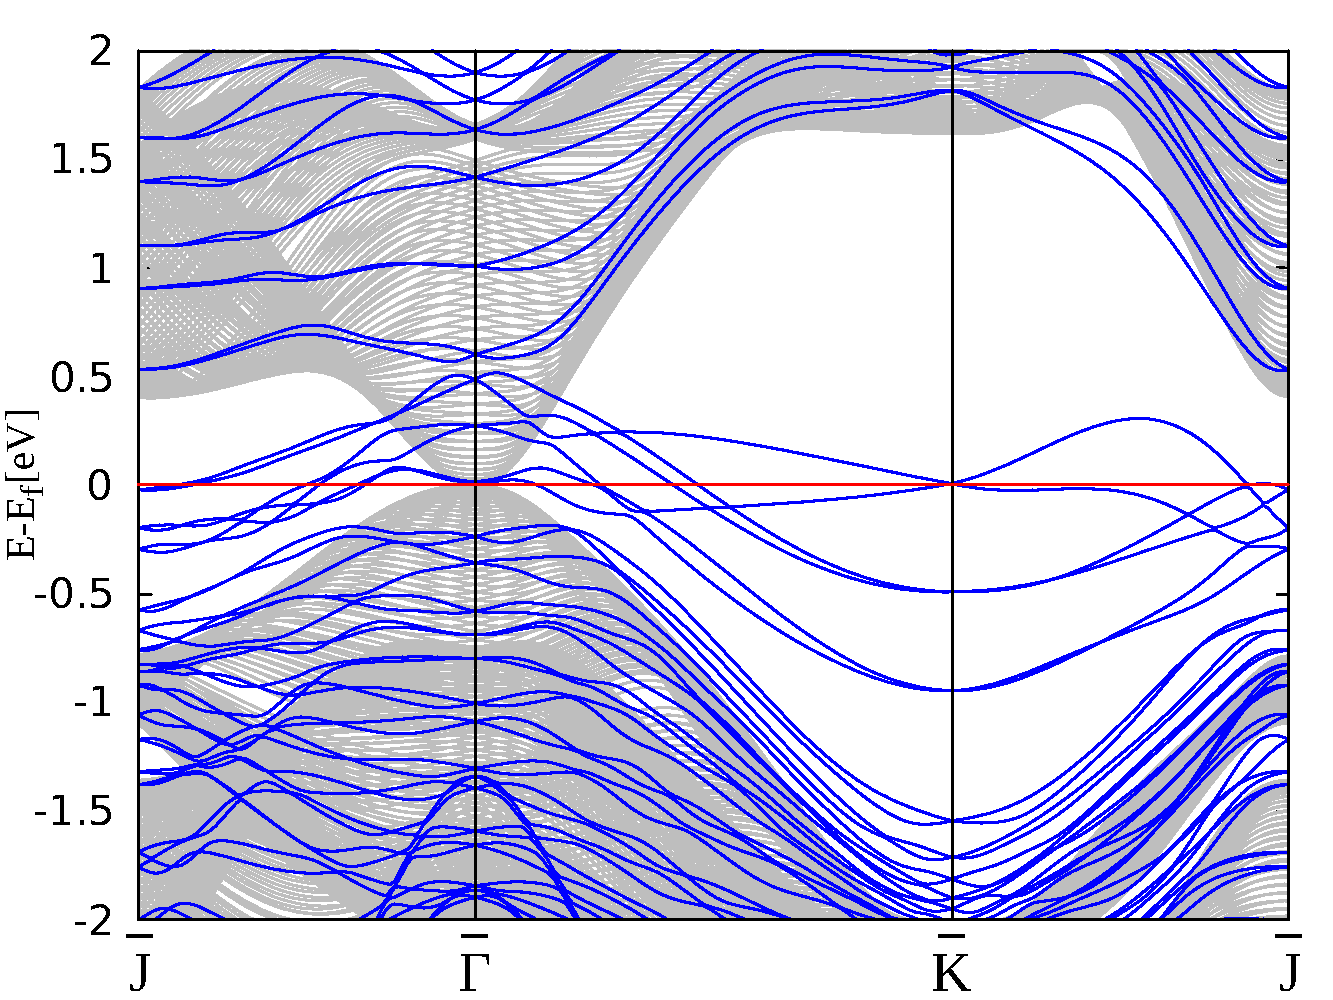
\includegraphics[width=\linewidth]{Te_and_Hg_termination/no_H_bulk+16_layers_no_dos_-2_2.pdf}
			\caption{16 layers without hydrogens passivating the Te termination} \label{}
		\end{subfigure}
		\hfill
		\begin{subfigure}[c]{.48\linewidth}
			\centering
			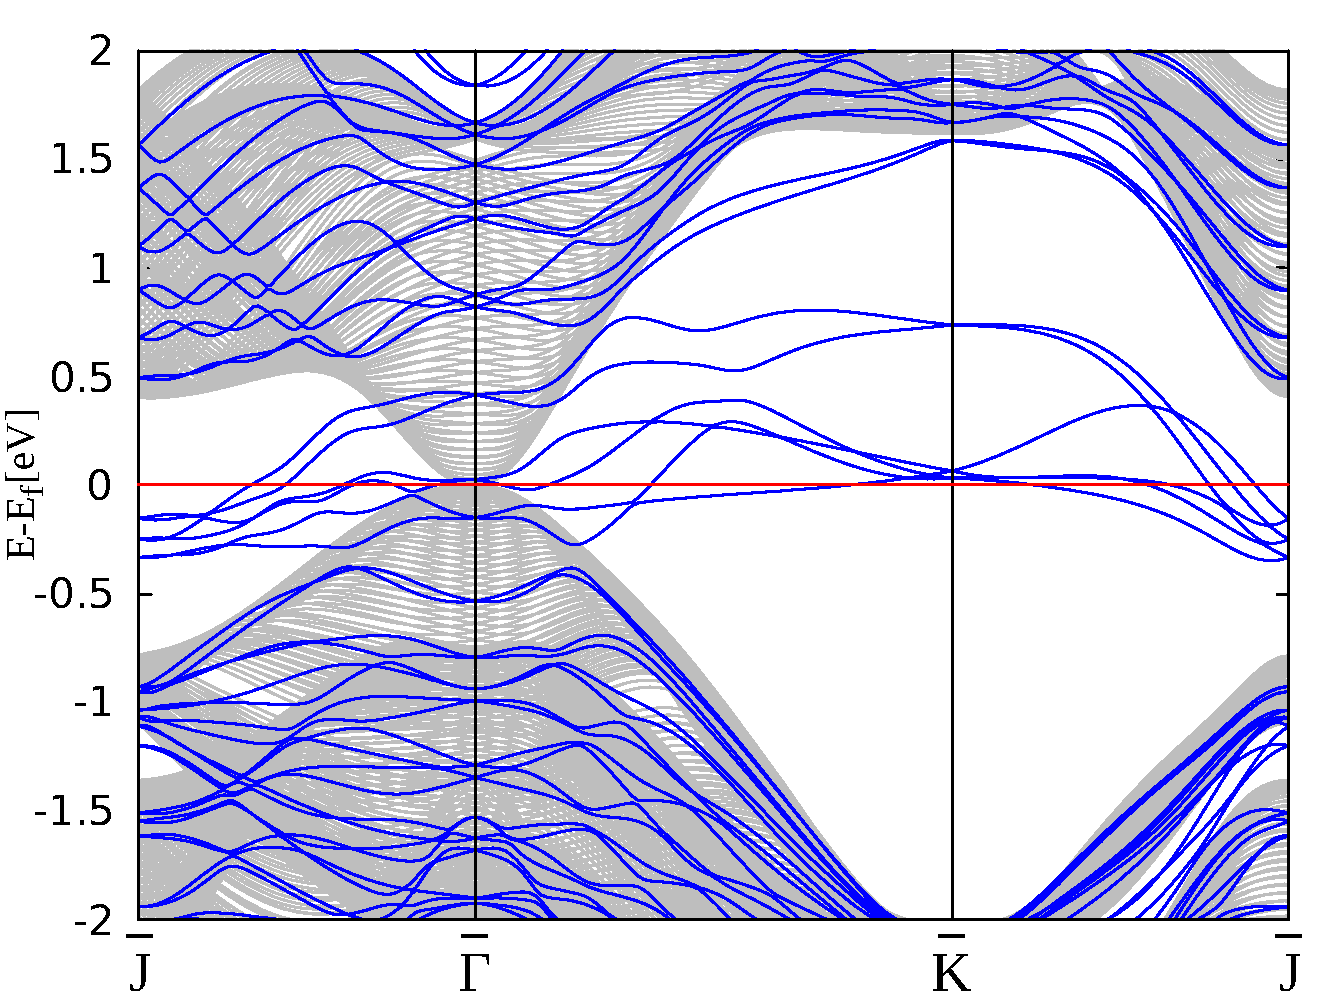
\includegraphics[width=\linewidth]{Te_and_Hg_termination/bulk+16_layers_no_dos_-2_2.pdf}
			\caption{16 layers with hydrogens on the bottom passivating the Te surface terminations}
		\end{subfigure}
		\caption{PBBS and surface band structure for Te-Hg terminations} 
		\label{bulk+surface_even_layers}
	\end{figure}

%Te termination	
	\begin{figure}[htbp]
		\begin{subfigure}[c]{.48\linewidth}
			\centering
			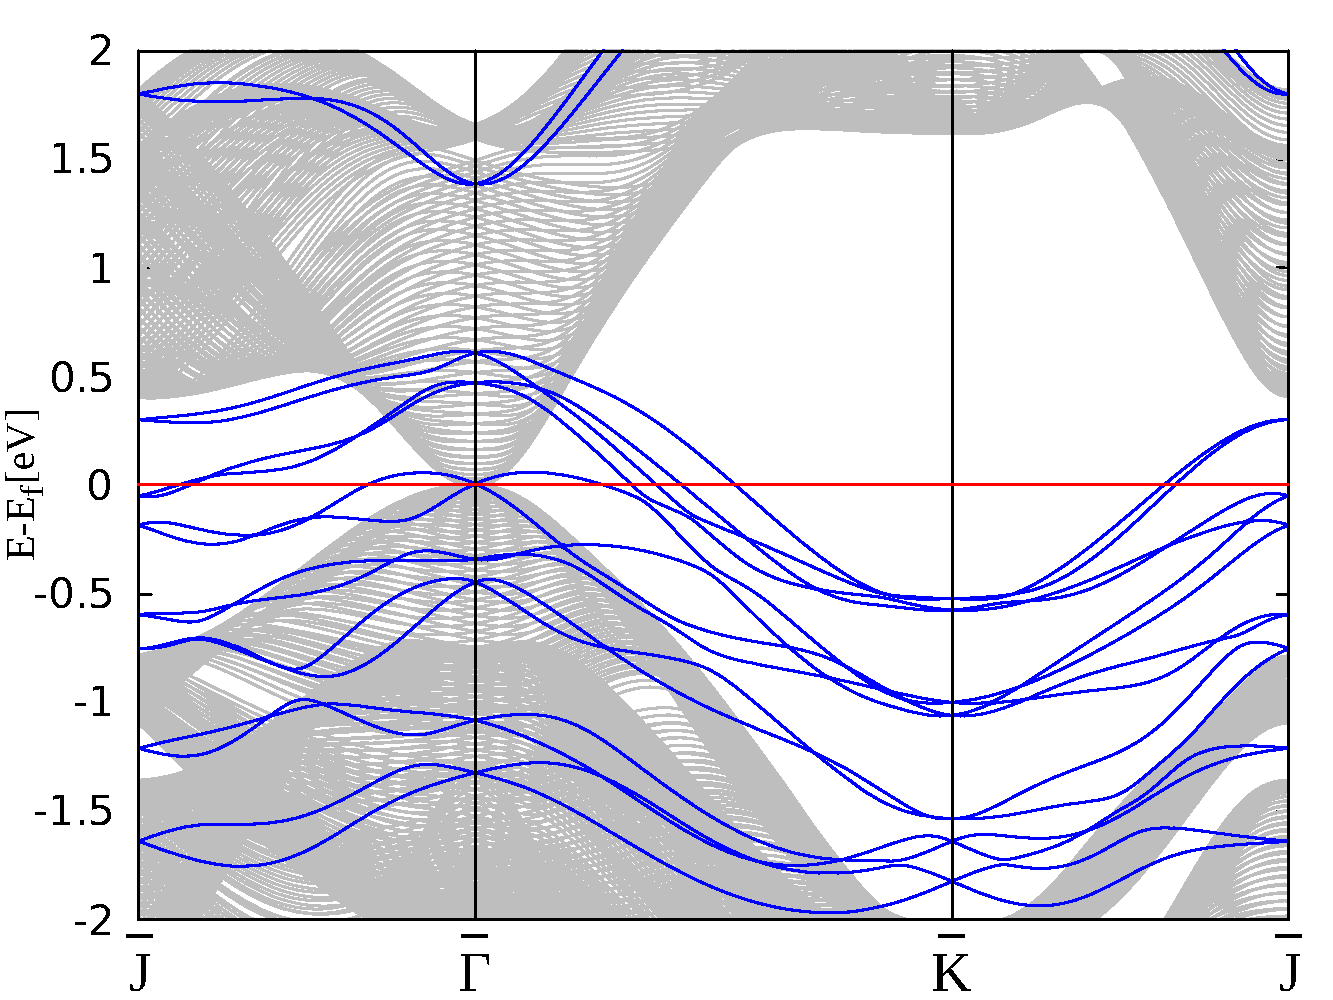
\includegraphics[width=\linewidth]{Te_termination/no_H_bulk+5_layers_no_dos_-2_2.pdf}
			\caption{5 layers without hydrogens passivating one of the surfaces}
		\end{subfigure}
		\hfill
		\begin{subfigure}[c]{.48\linewidth}
			\centering
			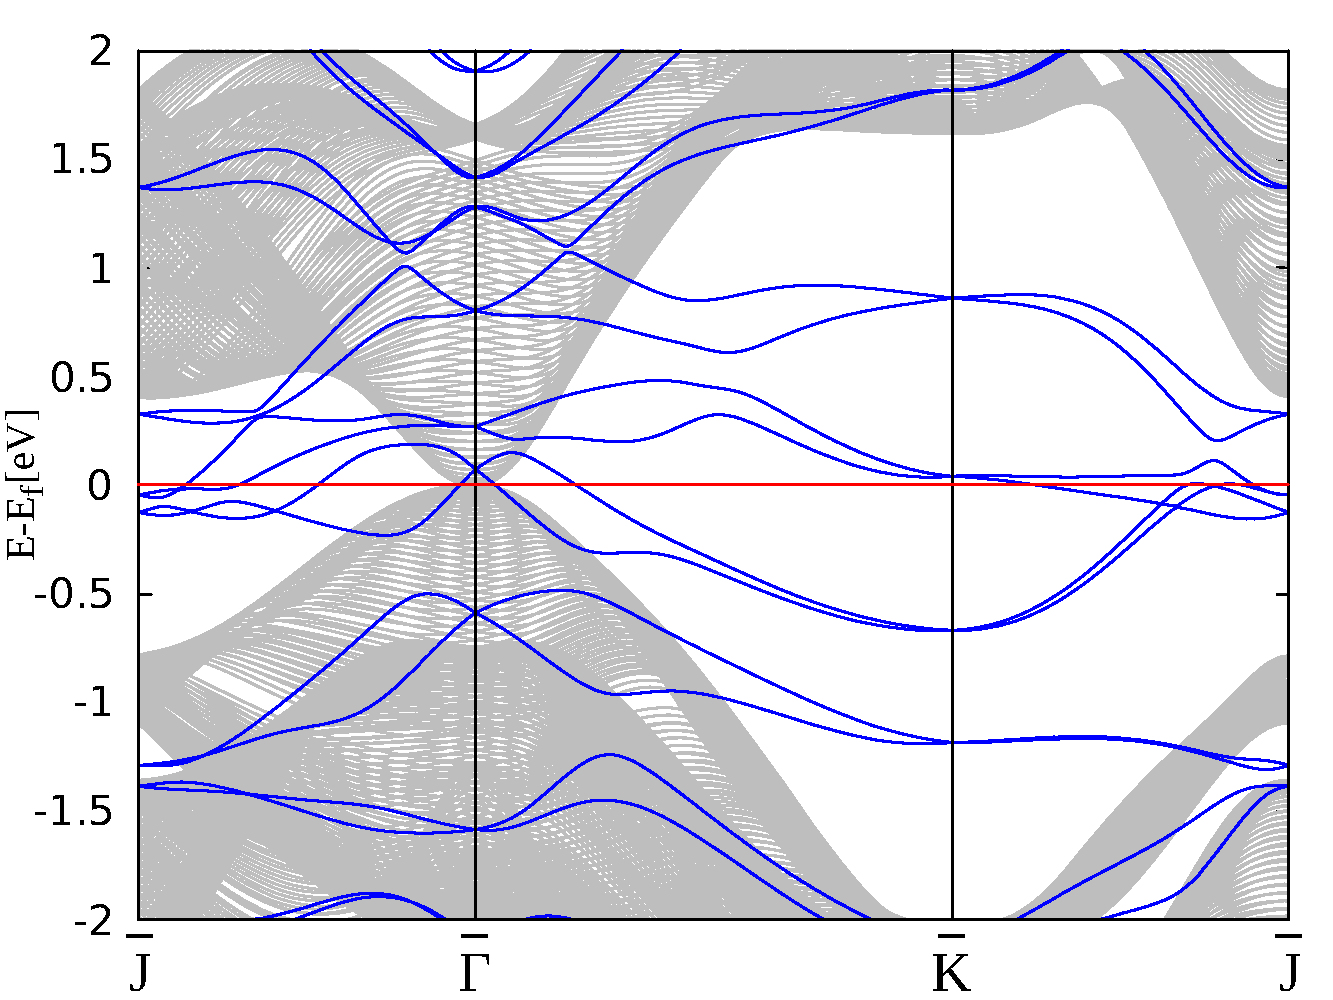
\includegraphics[width=\linewidth]{Te_termination/bulk+5_layers_no_dos_-2_2.pdf}
			\caption{5 layers with hydrogens on the bottom passivating one of the Te surfaces terminations}
		\end{subfigure}
		\begin{subfigure}[c]{.48\linewidth}
			\centering
			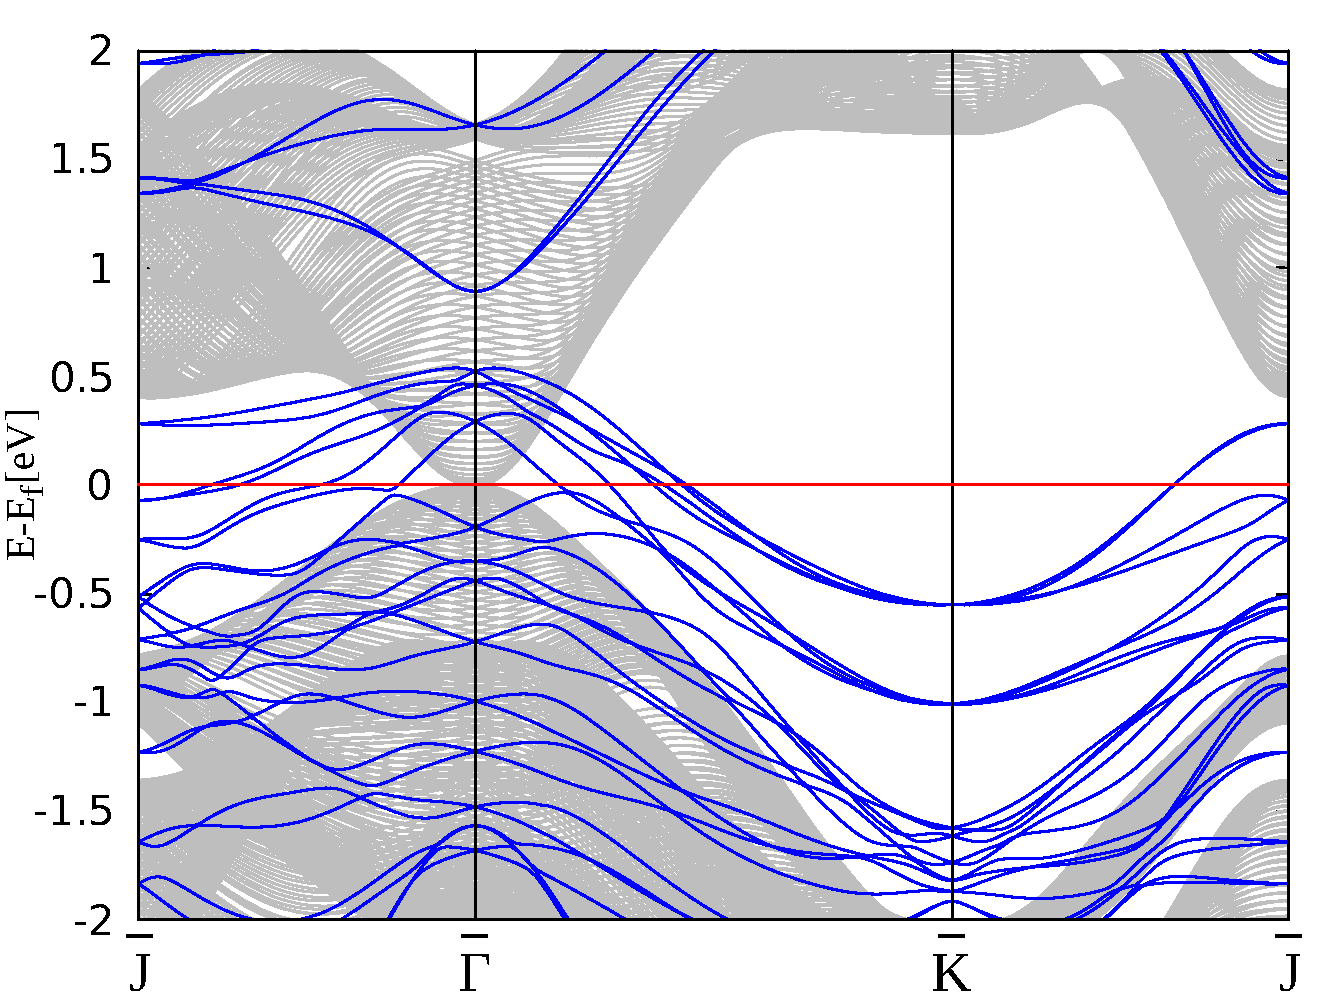
\includegraphics[width=\linewidth]{Te_termination/no_H_bulk+9_layers_no_dos_-2_2.pdf}
			\caption{9 layers without hydrogens passivating one of the surfaces}
		\end{subfigure}
		\hfill
		\begin{subfigure}[c]{.48\linewidth}
			\centering
			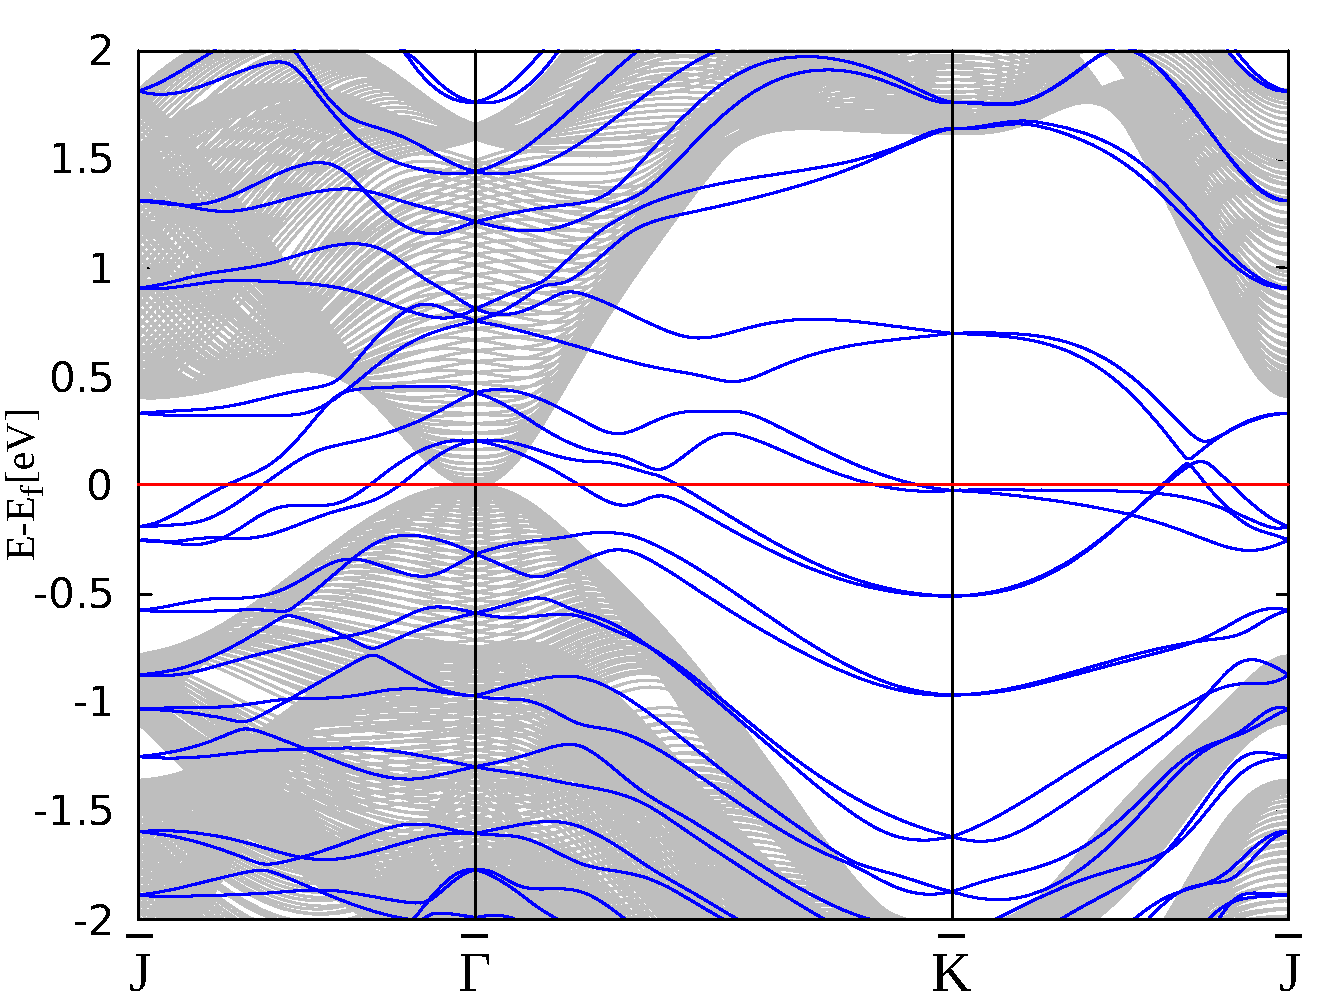
\includegraphics[width=\linewidth]{Te_termination/bulk+9_layers_no_dos_-2_2.pdf}
			\caption{9 layers with hydrogens on the bottom passivating one of the Te surfaces terminations}
		\end{subfigure}
		\begin{subfigure}[c]{.48\linewidth}
			\centering 
			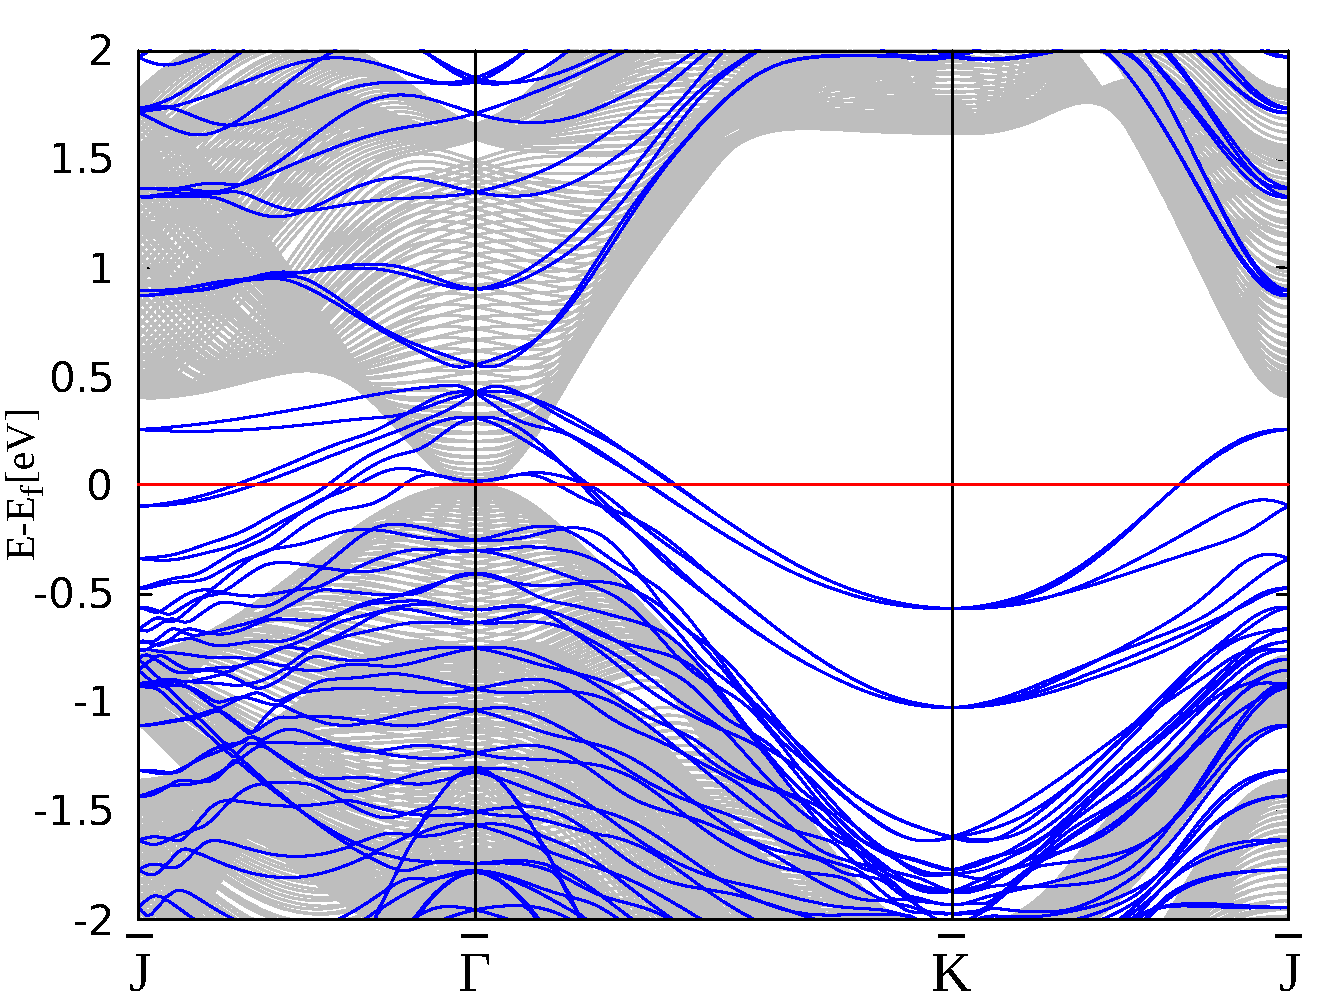
\includegraphics[width=\linewidth]{Te_termination/no_H_bulk+17_layers_no_dos_-2_2.pdf}
			\caption{17 layers without hydrogens passivating one of the surfaces} 
		\end{subfigure}
		\hfill
		\begin{subfigure}[c]{.48\linewidth}
			\centering
			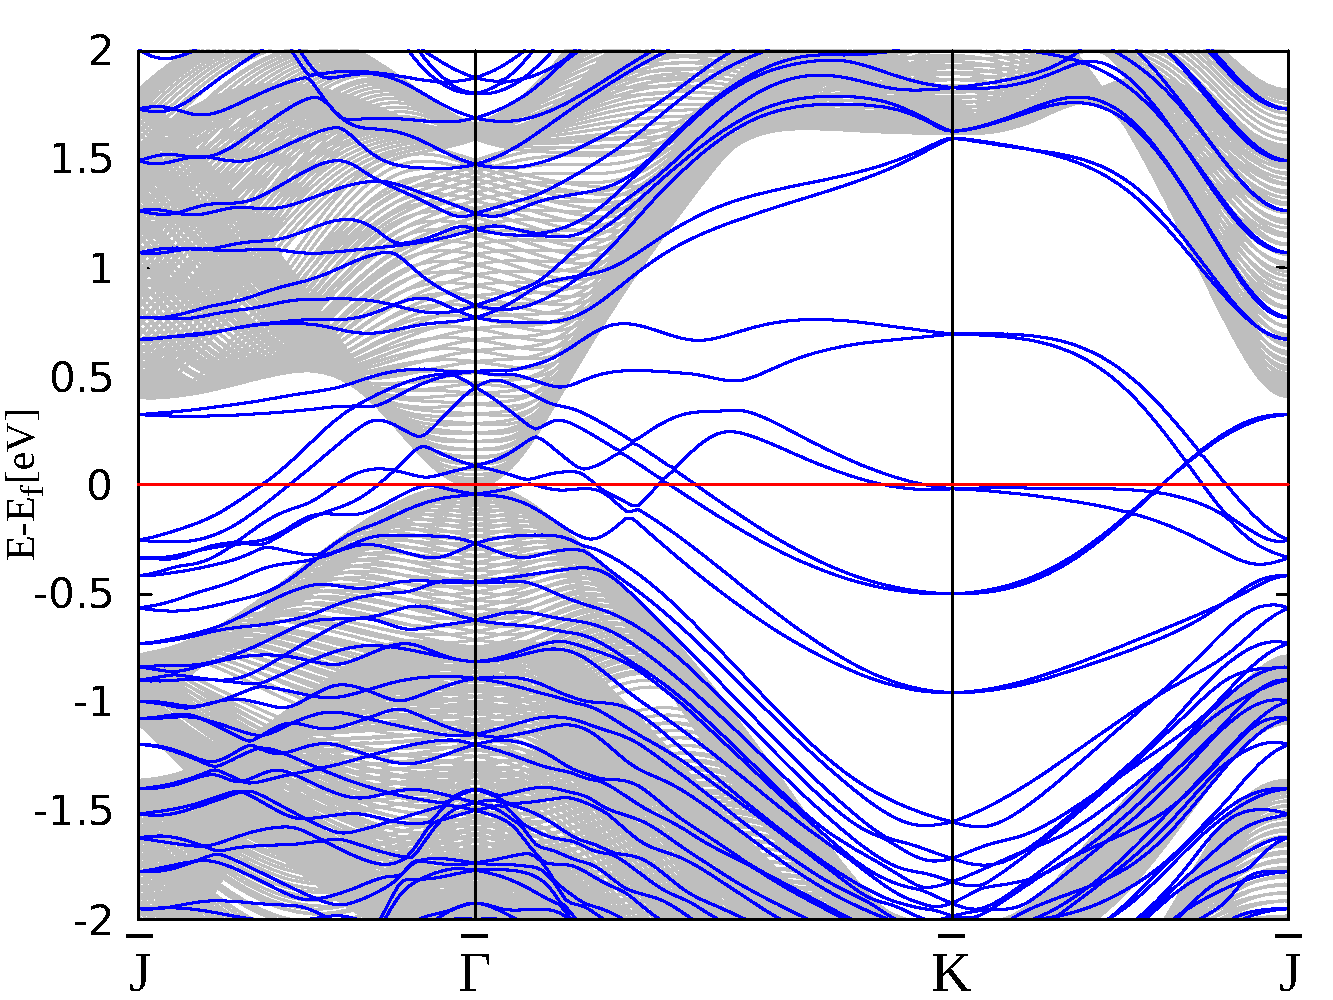
\includegraphics[width=\linewidth]{Te_termination/bulk+17_layers_no_dos_-2_2.pdf}
			\caption{17 layers with hydrogens on the bottom passivating one of the Te surfaces terminations}
		\end{subfigure}
		\caption{PBBS and surface band structure for symmetric Te termination on both surfaces of the slab} 
		\label{bulk+surface_odd_layers_Te}
	\end{figure}

%Hg termination	
	\begin{figure}[htbp]
		\begin{subfigure}[c]{.48\linewidth}
			\centering
			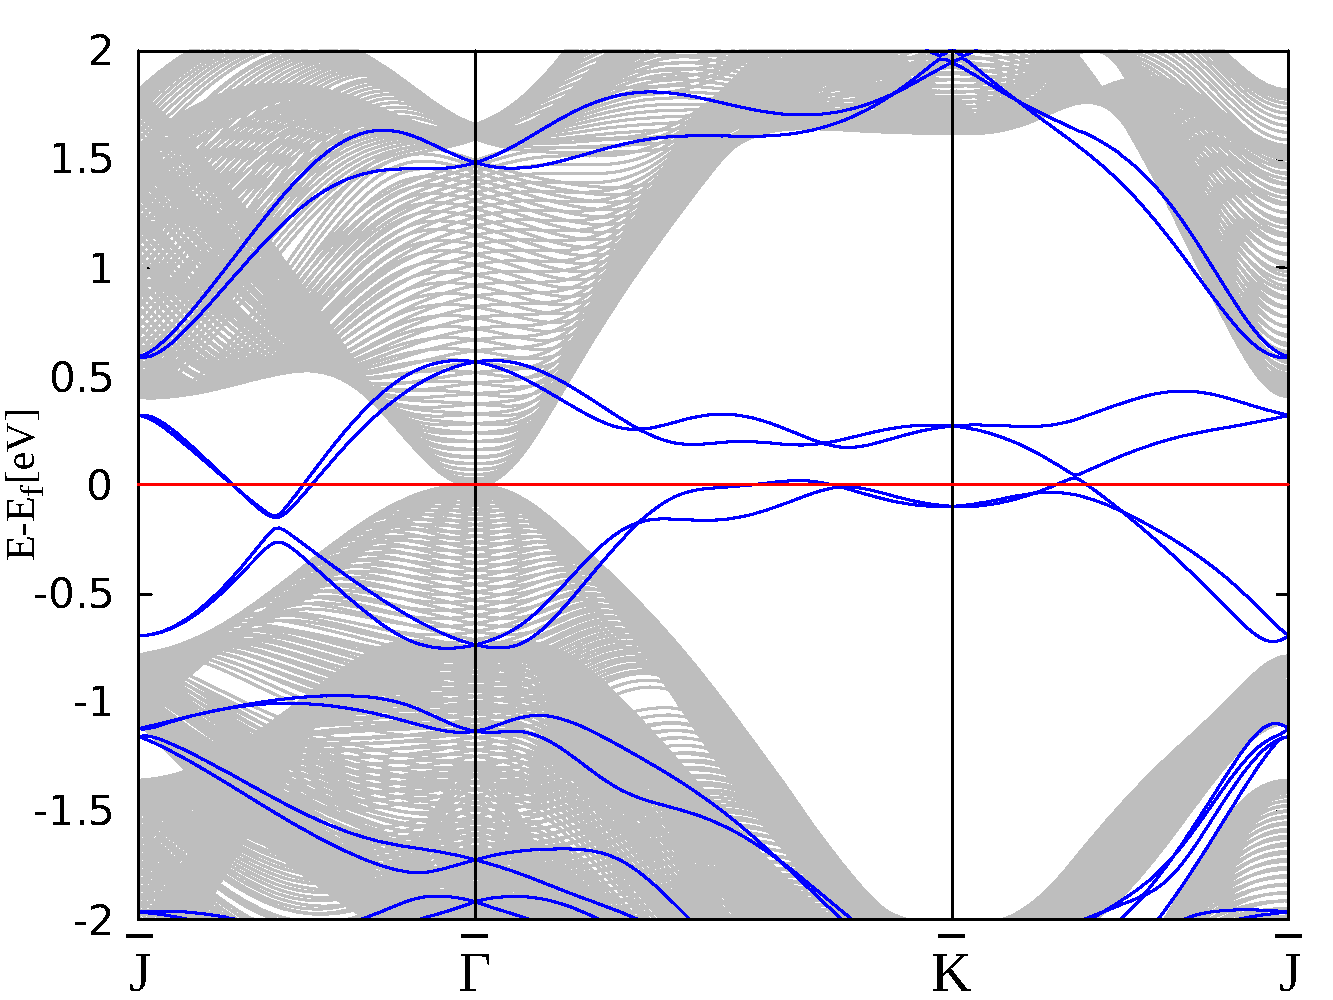
\includegraphics[width=\linewidth]{Hg_termination/no_H_bulk+5_layers_no_dos_-2_2.pdf}
			\caption{5 layers without hydrogens passivating one of the surfaces}
		\end{subfigure}
		\hfill
		\begin{subfigure}[c]{.48\linewidth}
			\centering
			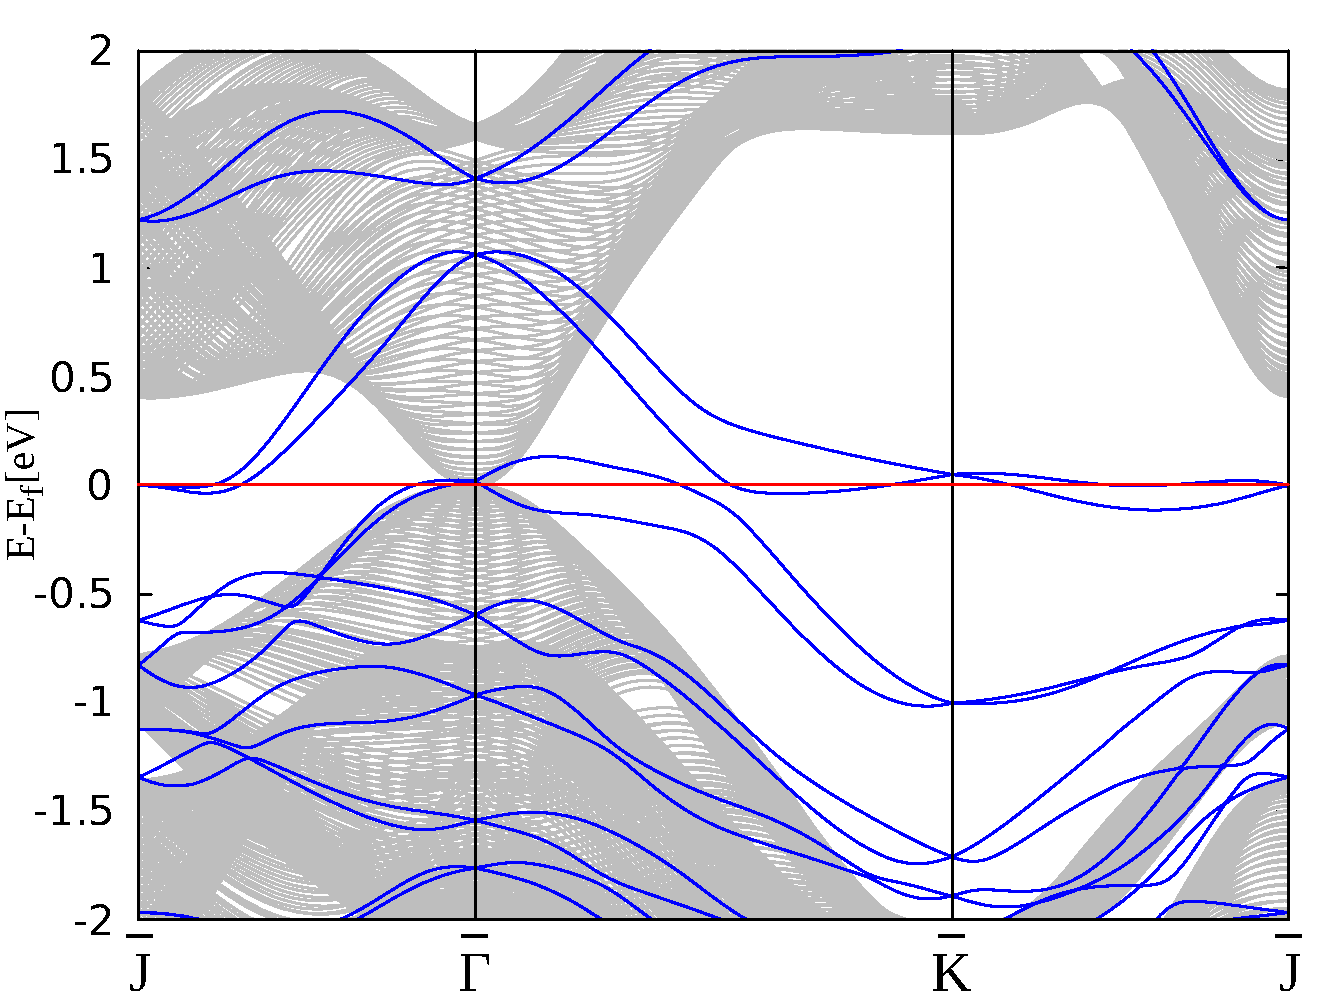
\includegraphics[width=\linewidth]{Hg_termination/bulk+5_layers_no_dos_-2_2.pdf}
			\caption{5 layers with hydrogens on the bottom passivating one of the Hg surface terminations}
		\end{subfigure}
		\begin{subfigure}[c]{.48\linewidth}
			\centering
			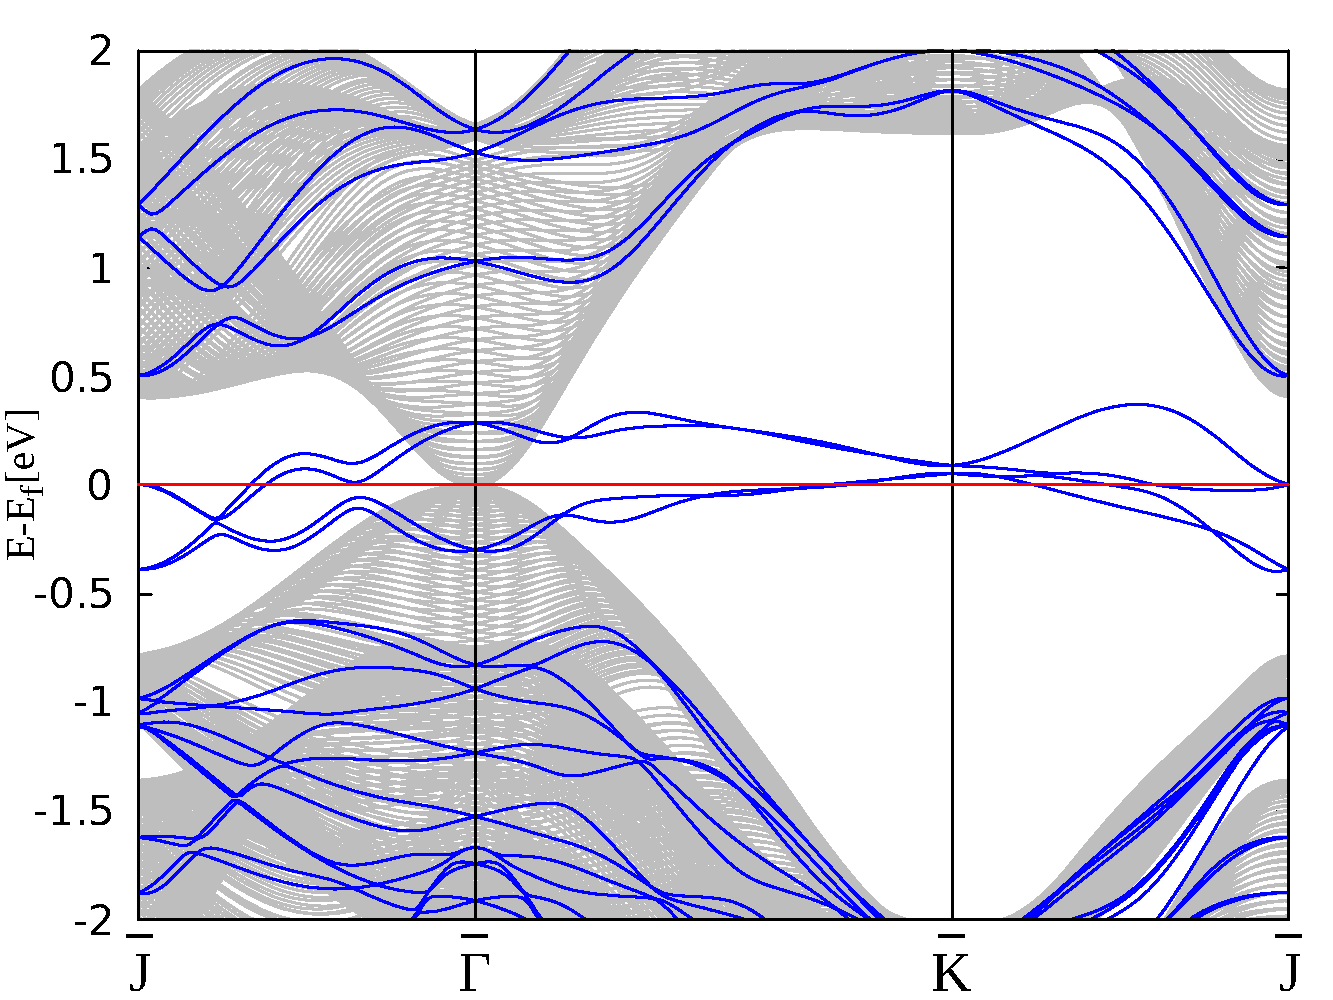
\includegraphics[width=\linewidth]{Hg_termination/no_H_bulk+9_layers_no_dos_-2_2.pdf}
			\caption{9 layers without hydrogens passivating one of the surfaces}
		\end{subfigure}
		\hfill
		\begin{subfigure}[c]{.48\linewidth}
			\centering
			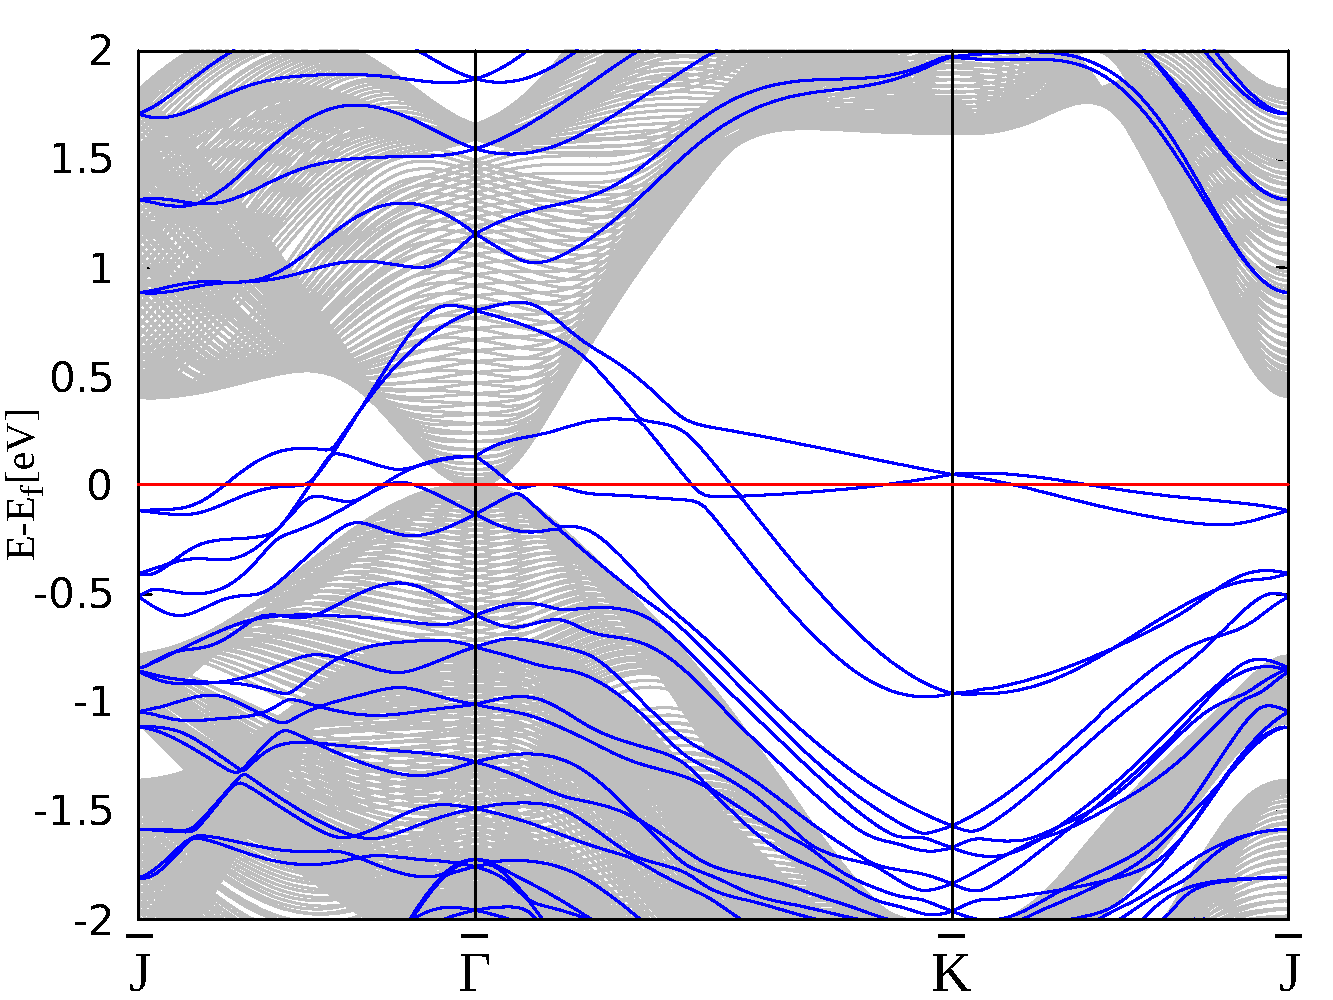
\includegraphics[width=\linewidth]{Hg_termination/bulk+9_layers_no_dos_-2_2.pdf}
			\caption{9 layers with hydrogens on the bottom passivating one of the Hg surface terminations}
		\end{subfigure}
		\begin{subfigure}[c]{.48\linewidth}
			\centering 
			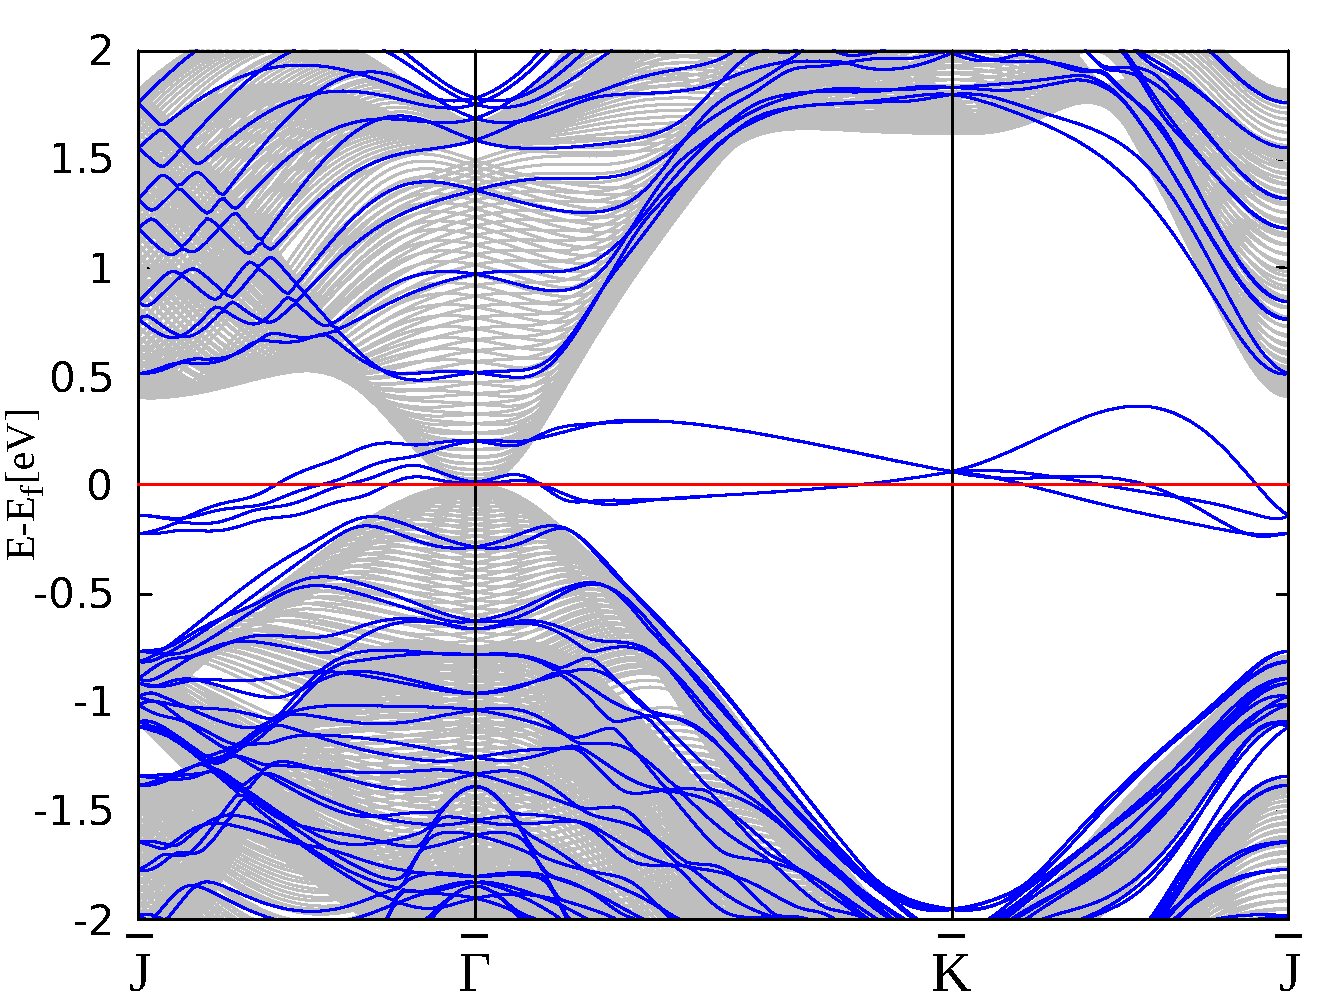
\includegraphics[width=\linewidth]{Hg_termination/no_H_bulk+17_layers_no_dos_-2_2.pdf}
			\caption{17 layers without hydrogens passivating one of the surfaces} \label{}
		\end{subfigure}
		\hfill
		\begin{subfigure}[c]{.48\linewidth}
			\centering
			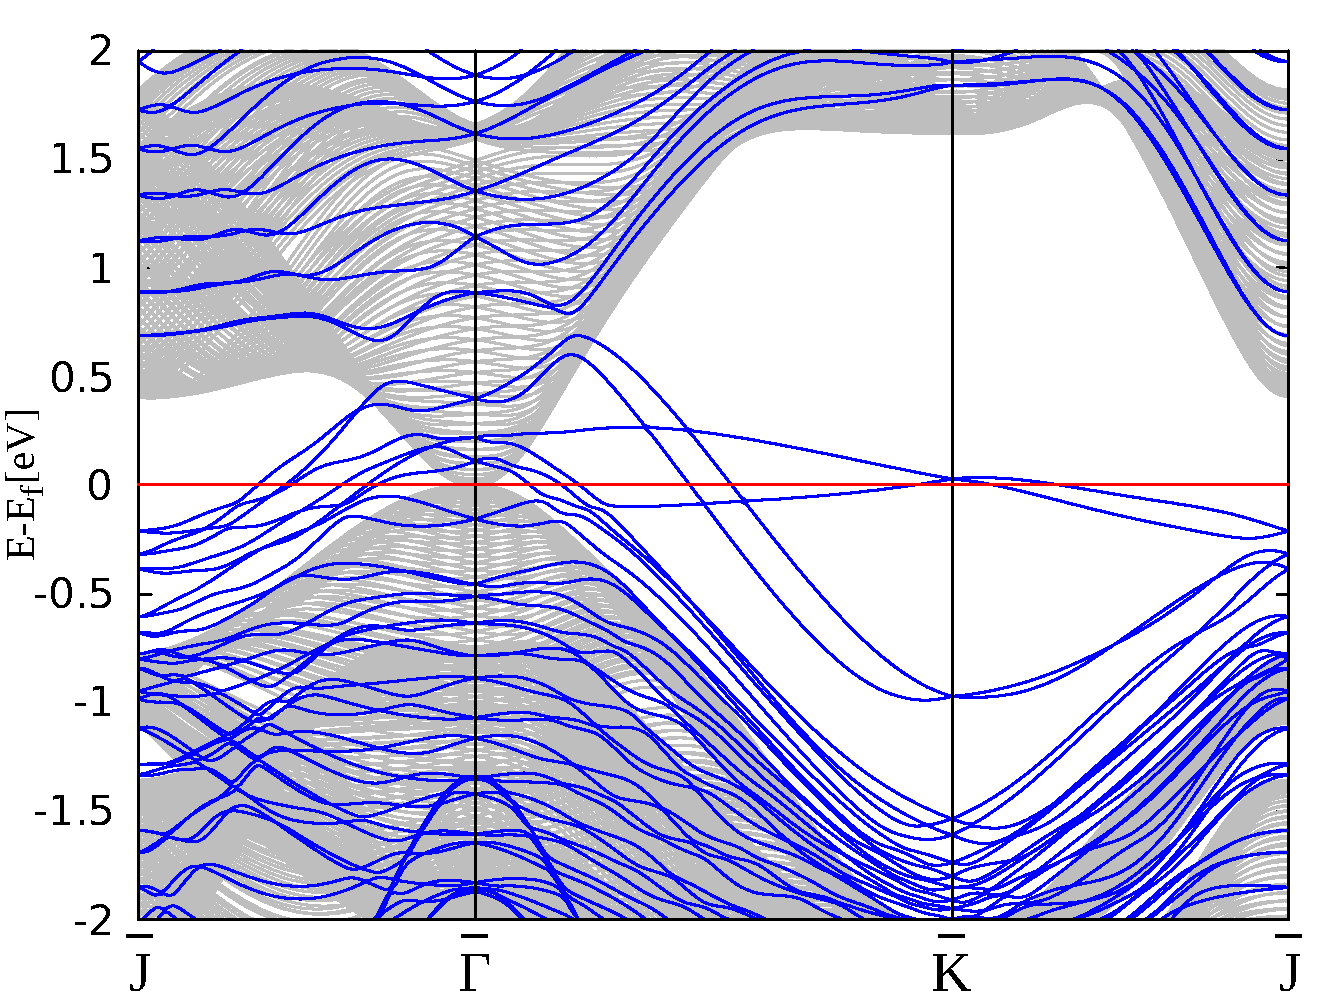
\includegraphics[width=\linewidth]{Hg_termination/bulk+17_layers_no_dos_-2_2.pdf}
			\caption{17 layers with hydrogens on the bottom passivating one of the Hg surface terminations}
		\end{subfigure}
		\caption{PBBS and surface band structure for symmetric Hg termination on both surfaces of the slab} 
		\label{bulk+surface_odd_layers_Hg}
	\end{figure}
	
%	\FloatBarrier
%	\subsection{Density of states}
%		\begin{figure}[tbp]
		\begin{subfigure}[c]{.48\linewidth}
			\centering
			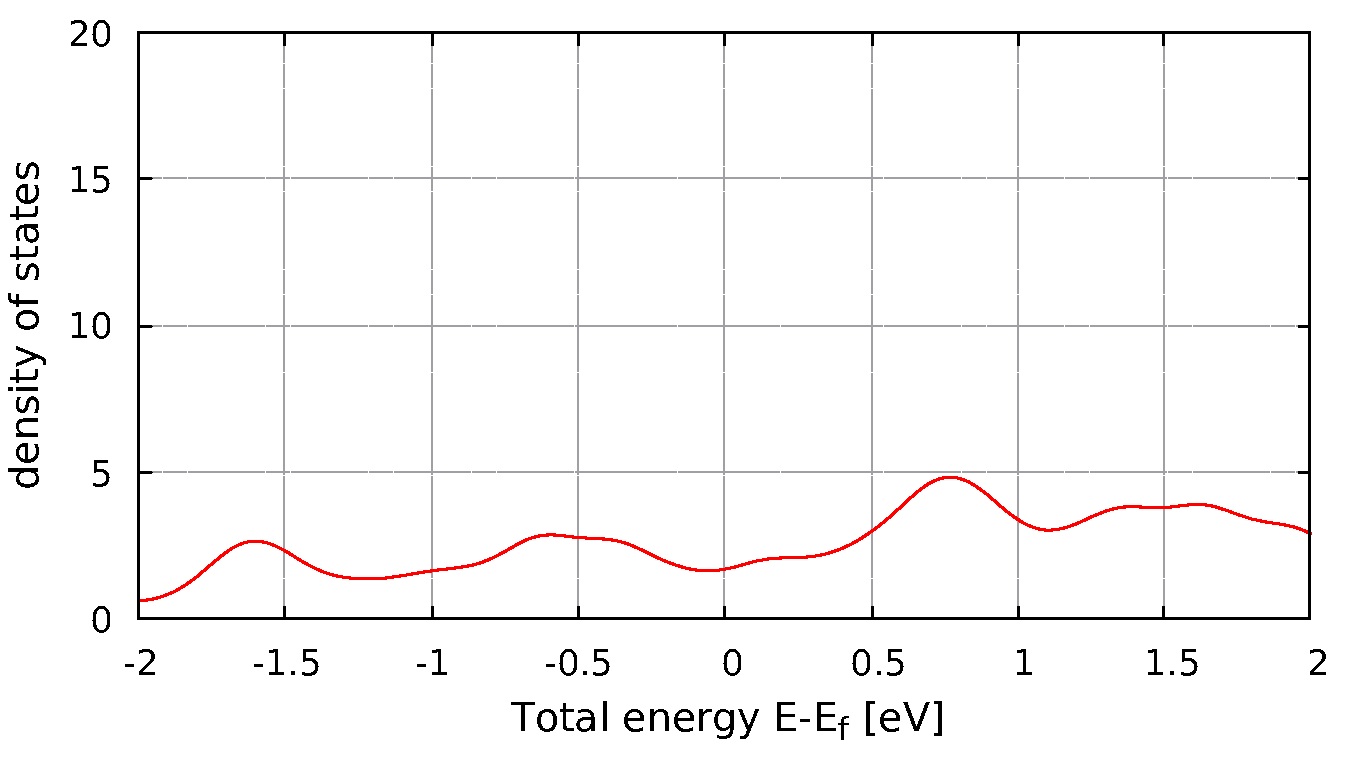
\includegraphics[width=\linewidth]{Te_and_Hg_termination/no_H_DOS_4_layers_-2_2.pdf}
			\caption{4 layers without hydrogens}
		\end{subfigure}
		\hfill
		\begin{subfigure}[c]{.48\linewidth}
			\centering
			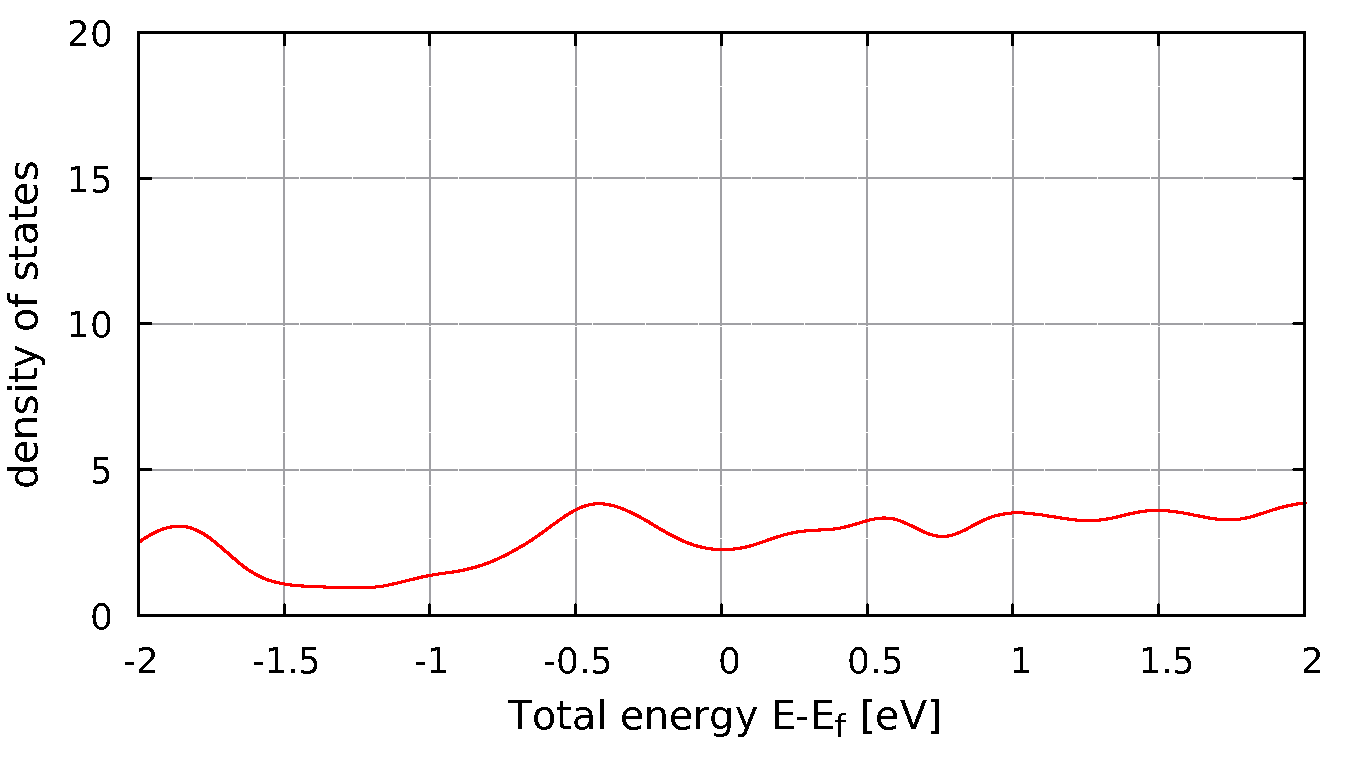
\includegraphics[width=\linewidth]{Te_and_Hg_termination/DOS_4_layers_-2_2.pdf}
			\caption{4 layers with hydrogens on the bottom}
		\end{subfigure}
		\begin{subfigure}[c]{.48\linewidth}
			\centering
			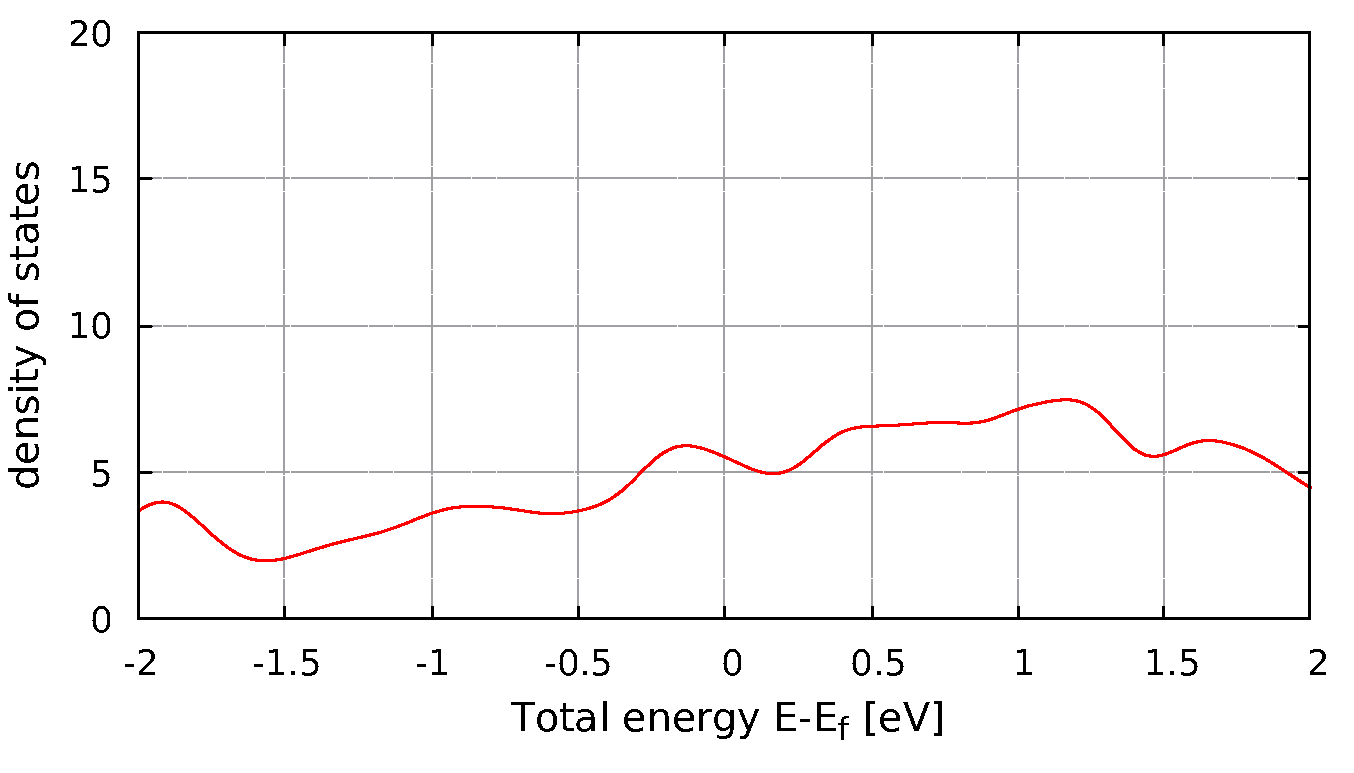
\includegraphics[width=\linewidth]{Te_and_Hg_termination/no_H_DOS_8_layers_-2_2.pdf}
			\caption{8 layers without hydrogens}
		\end{subfigure}
		\hfill
		\begin{subfigure}[c]{.48\linewidth}
			\centering
			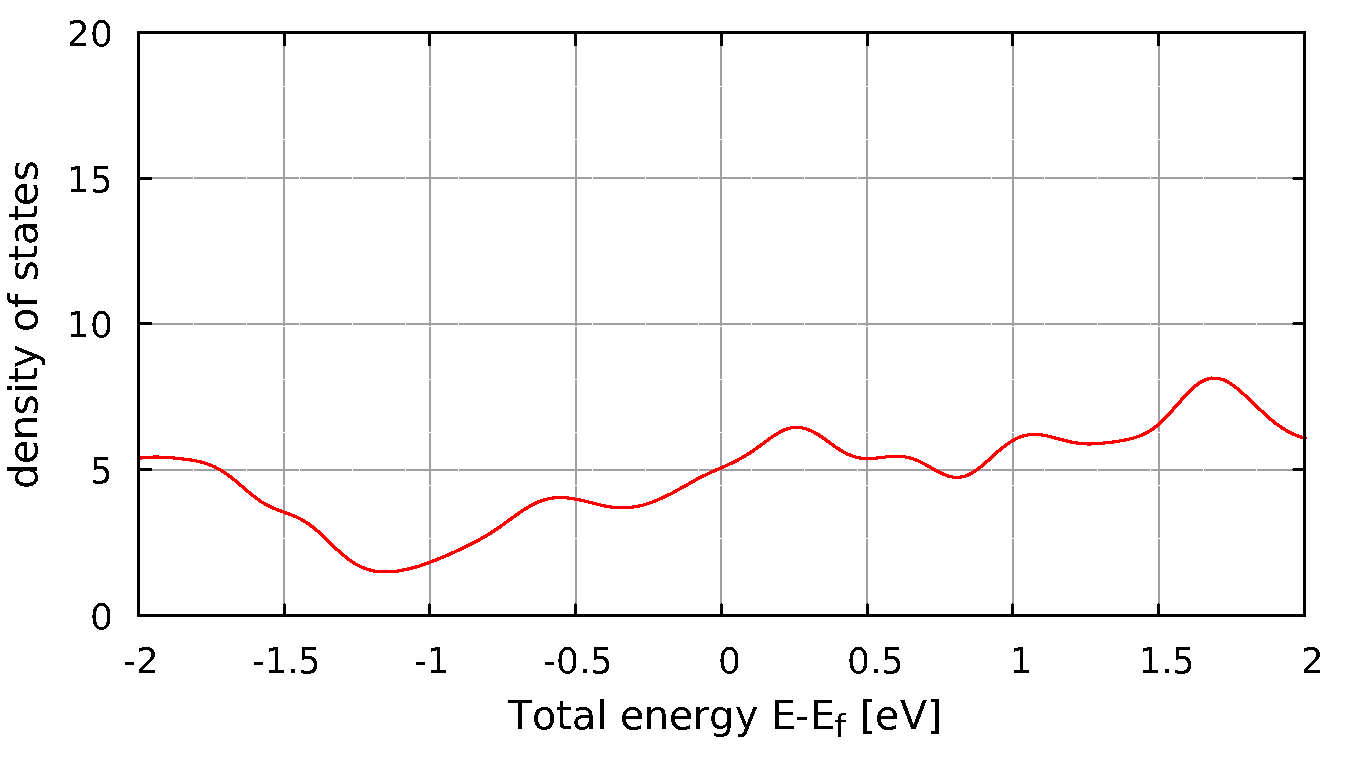
\includegraphics[width=\linewidth]{Te_and_Hg_termination/DOS_8_layers_-2_2.pdf}
			\caption{8 layers with hydrogens on the bottom}
		\end{subfigure}
		\begin{subfigure}[c]{.48\linewidth}
			\centering 
			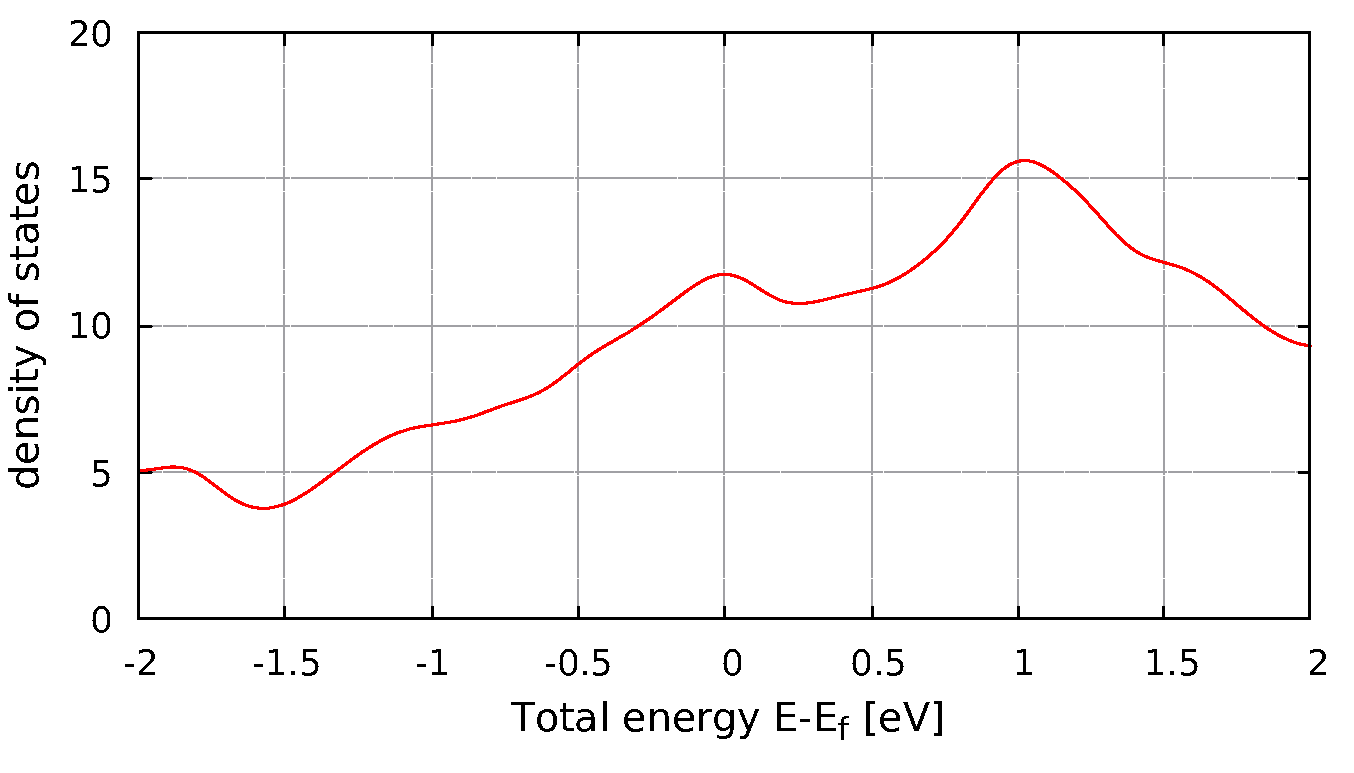
\includegraphics[width=\linewidth]{Te_and_Hg_termination/no_H_DOS_16_layers_-2_2.pdf}
			\caption{16 layers without hydrogens} \label{}
		\end{subfigure}
		\hfill
		\begin{subfigure}[c]{.48\linewidth}
			\centering
			\includegraphics[width=\linewidth]{Te_and_Hg_termination/DOS_16_layers_-2_2.pdf}
			\caption{16 layers with hydrogens on the bottom}
		\end{subfigure}
		\caption{DOS of the surfaces with Te-Hg termination} 
		\label{dos_surface_even_layers}
	\end{figure}

	\begin{figure}[tbp]
		\begin{subfigure}[c]{.48\linewidth}
			\centering
			\includegraphics[width=\linewidth]{Te_termination/no_H_DOS_5_layers_-2_2.pdf}
			\caption{5 layers without hydrogens}
		\end{subfigure}
		\hfill
		\begin{subfigure}[c]{.48\linewidth}
			\centering
			\includegraphics[width=\linewidth]{Te_termination/DOS_5_layers_-2_2.pdf}
			\caption{5 layers with hydrogens on the bottom}
		\end{subfigure}
		\begin{subfigure}[c]{.48\linewidth}
			\centering
			\includegraphics[width=\linewidth]{Te_termination/no_H_DOS_9_layers_-2_2.pdf}
			\caption{9 layers without hydrogens}
		\end{subfigure}
		\hfill
		\begin{subfigure}[c]{.48\linewidth}
			\centering
			\includegraphics[width=\linewidth]{Te_termination/DOS_9_layers_-2_2.pdf}
			\caption{9 layers with hydrogens on the bottom}
		\end{subfigure}
		\begin{subfigure}[c]{.48\linewidth}
			\centering 
			\includegraphics[width=\linewidth]{Te_termination/no_H_DOS_17_layers_-2_2.pdf}
			\caption{17 layers without hydrogens} \label{}
		\end{subfigure}
		\hfill
		\begin{subfigure}[c]{.48\linewidth}
			\centering
			\includegraphics[width=\linewidth]{Te_termination/DOS_17_layers_-2_2.pdf}
			\caption{17 layers with hydrogens on the bottom}
		\end{subfigure}
		\caption{DOS of the surfaces with Te termination} 
		\label{dos_surface_odd_layers_Te}
	\end{figure}
	
	\begin{figure}[tbp]
		\begin{subfigure}[c]{.48\linewidth}
			\centering
			\includegraphics[width=\linewidth]{Hg_termination/no_H_DOS_5_layers_-2_2.pdf}
			\caption{5 layers without hydrogens}
		\end{subfigure}
		\hfill
		\begin{subfigure}[c]{.48\linewidth}
			\centering
			\includegraphics[width=\linewidth]{Hg_termination/DOS_5_layers_-2_2.pdf}
			\caption{5 layers with hydrogens on the bottom}
		\end{subfigure}
		\begin{subfigure}[c]{.48\linewidth}
			\centering
			\includegraphics[width=\linewidth]{Hg_termination/no_H_DOS_9_layers_-2_2.pdf}
			\caption{9 layers without hydrogens}
		\end{subfigure}
		\hfill
		\begin{subfigure}[c]{.48\linewidth}
			\centering
			\includegraphics[width=\linewidth]{Hg_termination/DOS_9_layers_-2_2.pdf}
			\caption{9 layers with hydrogens on the bottom}
		\end{subfigure}
		\begin{subfigure}[c]{.48\linewidth}
			\centering 
			\includegraphics[width=\linewidth]{Hg_termination/no_H_DOS_17_layers_-2_2.pdf}
			\caption{17 layers without hydrogens} \label{}
		\end{subfigure}
		\hfill
		\begin{subfigure}[c]{.48\linewidth}
			\centering
			\includegraphics[width=\linewidth]{Hg_termination/DOS_17_layers_-2_2.pdf}
			\caption{17 layers with hydrogens on the bottom}
		\end{subfigure}
		\caption{DOS of the surfaces with Hg termination} 
		\label{dos_surface_odd_layers_Hg}
	\end{figure}
	The density of states (DOS) gives the number of states per interval of energy of a system which can be occupied in respect to specific energy levels \cite{tutorial2}.
	It gives no information about the actual occupation of states, but their availability. The higher the DOS at a specific energy, the more states are available there to be occupied. If the DOS is zero, there are no states able to be occupied. 
	
	In mathematical language: 
	By integrating over the energy $\epsilon$ within a unit volume cell in a small intervall $]\epsilon_0 - \Delta \epsilon , \epsilon_0 + \Delta \epsilon[$ and a certain function $g(\epsilon)$ which is called the density of states, the number of states are evaluated:
	\begin{align}
		n = \int_{\epsilon_0 - \Delta \epsilon}^{\epsilon_0 + \Delta \epsilon} \diff \epsilon g(\epsilon)
	\end{align}
	The density of states for free atoms or isolated molecules consists of dicrete energy levels, meaning it can be described by a delta function
	\begin{align}
		g(\epsilon) = \sum_i \delta(\epsilon_i - \epsilon)
	\end{align}
	For a periodic system the dos is k dependent which means, the integration of k must include the first Brillouin zone and must be averaged (divided by the volume)
	\begin{align}
		g(\epsilon) = \frac{1}{V_{BZ}} \sum_i \int_{BZ} \diff^3 k \delta (\epsilon_i(k) - \epsilon)  
	\end{align}
	But this equation is just brings exact results only for infinite k points. Since this is impossible to simulate by an numeric calculation, the infinite grid is replaced by a broadening of the delta distribution, concretely the Gaussion function with a factor $\sigma$:
	\begin{align}
		g(\epsilon) = \frac{1}{\sqrt{2\pi} \sigma} \frac{1}{n(k)} 
		\sum_i \sum_k \exp 
		\left[
			-\frac{1}{2} \left(
				\frac{\epsilon - \epsilon_i(k)}{\sigma}
			\right)^2
		\right]
	\end{align}
	The input command for FHI-aims must be set in the control.in by
	\begin{verbatim}
		# output DOS
		output dos -2. 2. 200 0.1
	\end{verbatim}
	where the first two numbers are the boundary values for the energy, the lower one first, the third is the number of energy value points taken for the integration, and the last one is the Gaussian broadening $\sigma$. 
	 
	The figures \ref{dos_surface_even_layers}, \ref{dos_surface_odd_layers_Te} and \ref{dos_surface_odd_layers_Hg} show the plots of the DOS calculations for every band structure plot that was done before. Note that the energy is now at the x axes and that the density of states the y axes in arbitrary units.   
	
%%% Local Variables:
%%% mode: latex
%%% TeX-master: "main_BA2.0"
%%% End:
%	 - What are you using as the Brillouin zone? How is your crystal? 
%	 - Reconstruction of the surface and what this means.
%	 - Talk about aims.
%	 - Show your results and how you got them:    
%	 Lattice convergence, k-grid study, etc.
%	 Band structures for the bulk
%	 Band structures for the surfaces (Put the comparison as well I mentioned previously with the atoms in the top moved and mention why you are doing this).
\FloatBarrier
\section{Interpretation of the results}	
\subsection{k-grid study}
	At the beginning of the calculations we demonstrated, that for the evaluation of the bulk HgTe the most economic k-grid setting for dividing the reciprocal space is 8x8x8. Note that for higher k-grids, which means smaller steps of discretization, more CPU time is required but would not harm the calculations. 
	
	The same study was performed on different slab thicknesses. Those results showed that the total energy as a function of k-grid steps was oscillating before it finally converged like the study did for the bulk. This oscillation has its origins in the broken translation symmetry in the direction perpendicular to the surface. The thinner the slabs is, the more apparent this side effect becomes because it affects more atoms per unit cell. 
%	Beginning with the k-grid outcome in figure \ref{k_grid_study}, the number points for the bulk must be at least 8, while a higher number is not necessary but doesn't harm the calculations either. 
%	In comparison to the $1/e^x$ like behavior of the bulk k-grid in \ref{k_grid_1}, the k-grid for the slabs does oscillate until the total energy converges at approximately 24 points in x and y direction is enough for 4 and 8 layers, see \ref{k_grid_2}, \ref{k_grid_3}. That oscillation calms down the larger the slabs become, hence the total energy converges earlier for 16 layers, see \ref{k_grid_4}, and the k-grid could be chosen smaller than for the thinner slabs. The reason for the bigger resemblance of thicker slabs to the bulk is, that the more layers the slab has, the more bulk-like it will be, because of the expansion in the third direction. This also applies to the band structure. 
%	
\subsection{Lattice constant study}	
	In subsection \ref{lattice_k-grid} we performed the study of the lattice constant for bulk HgTe. We showed that the minimum value of energy is reached at the lattice constant $a= 6.685 \,\unit{\AA}$. For comparison the experimental value at room temperature is $a=6.46152 \,\unit{\AA}$ and for LDA calculations, which was explained in subsection \ref{xc-func}, the value is $a= 6.346 \,\unit{\AA}$ (data from \cite{lattice_constant}).
%	For the investigation of the lattice constant with lowest rest energy, a high enough k-grid must be chosen, otherwise it would not necessarily converge, see figure \ref{kgrid_lattice_constant}. The outcome illustrated in figure \ref{lattice_constant} shows a minimum around 6.685 $\unit{\AA}$. For comparison the experimental value in room temperature is around 6.46152 $\unit{\AA}$, while DFT-LDA calculations come to 6.346 $\unit{\AA}$ and ab initio GGA, which is the topic of the method used here, are 6.656 $\unit{\AA}$ (all data taken from \cite{lattice_constant}). This means the evaluated lattice constant is units of hundredth Anström too big, thus the calculations brought a quite accurate result.
	
\subsection{Bulk band structure}
	We calculated the bulk band structure for HgTe with and without spin-orbit coupling for regarding the impact spin-orbit interactions have on mercury telluride. 
	%	Both plots are replica of result for the ones without SOC found in the literature \cite{bulk_bs}. 
	
	It seems that, because HgTe is made out of heavy elements, the calculations in which spin-orbit coupling is included are giving  physically meaningful results. Due to the spin-orbit interaction the original spin-degenerated bands are splitting up, as shown in figure \ref{bulk_band_structure}. 
	It is well known that for zinc-blende semiconductors the band splitting leads to a heavy hole band, a light gap band and a double degenerated conduction band near the $\Gamma$ point \cite{HgTe_structure_001} which is reproduced by our calculations. 
%	The band structure without using the SOC agree with the ones that can be found in several papers like in \cite {bulk_bs}. But the calculations only bring physically accurate results if the SOC is included and always differ from the band structure of non included SOC. Figure \ref{bulk_band_structure} mostly shows the band splitting due to the spin momentum locking which was explained in the theoretical part \ref{topological_insulator} and \ref{chapter_soc}.
	
\subsection{PBBS and the band structure of the slabs}
	In the main part we made the projected bulk band structure which represents the energy dispersion relation for electrons in HgTe. Therefore we calculated the dispersion relation for different $k_z$ in order to study slices of the first 3D Brillouin zone. In our case we concentrate on the (001) direction. As mentioned before in subsection \ref{surface_modeling}, this the growing direction of the slabs on which we want to analyze the potentially topological surface states. The plot for the projected bulk band structure in $k_z$ direction is shown in figure \ref{bulk_band_structure_generation}.  The grey area correlates to the energy values an electron can adopt if one is looking on the bulk band structure from $k_z$ direction. Note that this only gives information about the bulk. 
	
	Therefore we calculated the band structures for the slabs with different thickness and terminations at the surfaces. Note that the Fermi energy was set to zero and that we only regarded ideal surfaces. Of course we see the band splitting caused by the spin-orbit interaction, seen in the bulk band structure, also in the slab surface bands.
	
	After we superimposed the band structures of the slabs and the PBBS, we noticed that the slab bands appear in the white area of the PBBS as well as in the grey area, which belongs to the bulk. 
	The bands of the slabs, which are in the grey region, are bulk energy bands while the slab bands which cross the white area, the band gap of the bulk, are the surface states. The latter can be either trivial or topological surface states, which we can distinguish by looking where those bands come from and where they go to. A band can only represent a topological surface state if the band comes from the valence/conduction band and goes to the conduction/valence band. 
	Additionally one can count how many times the dispersion line crosses through the Fermi level. If the number of crossings is odd, then this energy band is a topological surface state \cite{Bansil}.
	
	By looking at figure \ref{bulk+surface_even_layers}, \ref{bulk+surface_odd_layers_Te} and \ref{bulk+surface_odd_layers_Hg} we notice that the slab band structure is very sensitive under variation of thickness and terminations. It stands out, that the number of bands rises as the slabs are becoming thicker. In the plots for 16 and 17 layers we find energy bands which lie entirely within the PBBS. These represent the bulk states. On the contrary the bands lying completely in the band gap are the surface states which can be seen clearly in figure \ref{bulk+surface_even_layers}, \ref{bulk+surface_odd_layers_Te} and \ref{bulk+surface_odd_layers_Hg} in (e) and (f). 
	
	Since we turn our attention particularly to the evolution of the topological surface states, we observe that the structure of the dispersion relation differs much for different surface terminations. 
	Regarding the slabs with one surface passivated by hydrogens, then we see that the energy bands corresponding to the surface states are shifted away from the Fermi level \cite{top_surf_states}. In the plots for clean terminations one can observe possible candidates for a Dirac cone.
	
	By counting all crossings of the dispersion energy through the Fermi level we only discover trivial surface states. This is provoked by the dangling bonds at the crystal's surface. 
	In order to see topological surface states we could just use strained HgTe like in \cite{HgTe_structure_001} or use the c(2x2)-type reconstruction like in \cite{top_surf_states}. In the latter case they studied Te-terminated slabs and found Dirac cones at the $\Gamma$ point once strain was applied and semi-infinite slabs were studied. For symmetric Hg-terminations they found Dirac cones at $\overline{\text{K}}$ and $\overline{\text{J}}$ in (001) direction in case of clean surfaces. 
	The hydrogens effects the isotropic Dirac cone in a way that they become anisotropic cones.  
	
	The reconstruction of the surfaces, the simulation of strains and the simulation of semi-infinite surfaces is beyond this bachelor thesis. 
%	Regarding the left column in the figures \ref{bulk+surface_even_layers}, \ref{bulk+surface_odd_layers_Te} and \ref{bulk+surface_odd_layers_Hg}, there are four bands, means eight states, near the Fermi level which belong to the surface. The four upper states are unoccupied and separated from the bulk, while the lower states merge with the bulk at some point. Their shape depend on the terminations. For example in the Te-Hg termination plots \ref{bulk+surface_even_layers} on the left side, the band which crosses the Fermi level at the $\overline{\text{K}}$ point, can be found in the left column of the Hg termination \ref{bulk+surface_odd_layers_Hg}. In contrast, the other bands which traverse the $\overline{\text{K}}$ point below the Fermi level but still not in the bulk, are only found again in the Te-termination plots \ref{bulk+surface_odd_layers_Te} (information from \cite{top_surf_states}).
%
%	In the right part of those band structures, there can be seen, that part a part of those surface states near the Fermi level are shifted away from that level. The reason is the passivation of the danging bonds of the lower surface. Because just one of the two surfaces is occupied by hydrogens, just half of the bands are shifted. And also here conformities between the mono-atom termination and the Te-Hg termination can be found. 
%	
%	Regarding the $\overline{\Gamma}$ point, most small layered slabs do not have an s-like surface band at the Fermi level which would be typical for an inverted band structure in topological insulators \cite{2D_top_ins}, just in case of Te terminated 5 layer slabs, the Hg terminated 5 layer slab with hydrogens and in nearly all 16 or 17 layer slabs except the Hg terminated and hydrogen occupied 17 layer slab. This means the band gap does not contain s-like states at Fermi level in all other slabs. 
%	
%	The hydrogen occupation leads not only to the band shift but also to more space between the bands. The anisotrophy of the Dirac cone disappears and the occupied dangling bonds no longer support an conducting surface. 
	
%	\subsection{Density of states} 
%	As one can see in all dos plots \ref{dos_surface_even_layers}, \ref{dos_surface_odd_layers_Te} and \ref{dos_surface_odd_layers_Hg}, there is no band gap in which the dos would be zero but in the 5 and 9 layer slabs without hydrogens with Te termination the dos approaches zero and gives rise to assume a band gap. The Te terminated 17 layer slab without hydrogens there is a slump near the Fermi level which is missing in the Te-Hg termination because at the same place in the Hg terminated slab there is a climax in the dos. It seems, that for hydrogen occupied surfaces, the dos plots get smother and the peaks lower but, since above the Fermi level the dos is in general higher than in the ones for no hydrogens added slabs, it can be assumed that the availability of states in the conduction band is better than for no hydrogens. 
	
	
%	, only the thickest slabs, meaning containing 16 or 17 layers, without hydrogens having a surface band at the Fermi level.
		
%	 Here you have to explain all what I indicated in the previous emails. (Don't forget about the DOS): How are the bulk band structure and the band structures for the surfaces related?
\section{Conclusion}
	In this thesis we performed ab-initio calculations for the dispersion energy in case of thin HgTe films with different thicknesses and terminations. These slabs were regarded as grown in the crystallographic (001) direction.
	
	We compared the bulk band structures in which we did or did not include the spin-orbit coupling and showed that band splitting can be observed by including the spin-orbit interactions.
	The superimposing of the slab energy bands and the projected bulk band structure in (001) direction allowed us to identify the surface states and additionally to discuss the topological character of HgTe in that direction. 
	After analyzing the surface band structure we discovered that, because of the dangling bonds at the surface, all of them are trivial surface states. 
	
	Finally we pointed out that for strained HgTe or for surface reconstruction of Hg- and Te-terminations the observation of topological surface states is possible. 
%	In the first part of the results, the k-grid study converged as wanted, the lattice constant study had a minimum for higher k-grid so the lattice constant had been determined to 6.685 $\AA$. After this part, the band structure in the three-dimensional Brillouin zone for the bulk was calculated with and without spin-orbit coupling on the one hand for pointing out the difference between them, on the other hand for making sure that FHI-aims includes the spin-orbit coupling.
%	
%	Then the slab band structure were calculated in respect to the projected bulk band structure to identify the surface states and their development during the growth of the HgTe crystal. This was then complemented by the examination of the density of states in the same energy area. 
%	
%	On the whole all results were confirming existing studies and showed that the characteristic surface states of the topological insulator HgTe are visible for thin layers.
\newpage
\FloatBarrier
\thispagestyle{empty}
\printbibliography
\end{document}

%%% Local Variables:
%%% mode: latex
%%% TeX-master: "main_BA2.0"
%%% End: